\documentclass[utf8, russian, hpadding=5mm, vpadding=15mm, floatsection, columnxxvi, columnxxxi, columnxxxii, equationsection, pointsection, footnoteasterisk]{eskdtext}

%доп. пакеты
\usepackage{amsfonts, amsmath, amssymb}	%Для математических штуковин
\usepackage{wallpaper}					%Для вставки сторонних страниц
\usepackage{array}						%Доп. возможности у таблиц

\usepackage{color}
\usepackage{stfloats}
\usepackage{bm}
\newcommand{\vect}[1]{\boldsymbol{\mathbf{#1}}}
\usepackage{arydshln}
\usepackage{tabularx}
\newcolumntype{Y}{>{\centering\arraybackslash}X}
%доп. настройки
\bibliographystyle{ugost2008}					%Стиль списка литературы
\graphicspath{{./images/}{./extra_pdf_pages/}}	%Папки с картинками

%на случай, если команда не определена
\newcommand{\No}{\textnumero}

\usepackage[]{algorithm2e}

\usepackage{listings}
\lstset{language=Python,basicstyle=\scriptsize}
\lstset{language=C,basicstyle=\scriptsize}

\lstdefinestyle{customc}{
	belowcaptionskip=1\baselineskip,
	language=C,
	showstringspaces=false,
	basicstyle=\footnotesize\ttfamily,
	keywordstyle=\bfseries\color{green!40!black},
	commentstyle=\itshape\color{purple!40!black},
	identifierstyle=\color{blue},
	stringstyle=\color{orange},
}
\lstset{escapechar=@,style=customc}


%определения своих команд
\DeclareMathOperator{\atan2}{atan2}
\DeclareMathOperator{\sign}{sign}
\DeclareMathOperator{\diag}{diag}
\newcommand{\msf}[1]{\mathsf{#1}}    %определение короткого обозначения для спец. начертания в формулах
\newcommand{\nv}{\mathbf0}           %нулевой вектор
\newcommand{\ds}{\displaystyle}      %короткое обозначение для размера символов в формулах

%для определения форматирования нумерации элементов списка литературы
\makeatletter
\renewcommand{\@biblabel}[1]{#1}
\makeatother

%для штампа
\ESKDtitle{\footnotesize Робототехническая система с техническим зрением для манипуляции подвижными объектами\\ \small Пояснительная записка}
\ESKDsignature{КСУИ.106.4235.001 ПЗ}
\ESKDgroup{\footnotesize Университет ИТМО\\Кафедра СУиИ\\гр.~P4235}
\ESKDauthor{\resizebox{2.22cm}{\height}{Артемов К.}}
\ESKDchecker{\resizebox{2.22cm}{\height}{Капитонов А.А.}}
\ESKDnormContr{\resizebox{2.22cm}{\height}{Быстров С.В.}}
\ESKDapprovedBy{}

%оступы от заголовков разделов и подразделов
\ESKDsectSkip{section}{7mm}{7mm}
\ESKDsectSkip{subsection}{5mm}{5mm}
\ESKDsectSkip{subsubsection}{1mm}{1mm}

\begin{document}
\addtocounter{page}{1} %если в документ будут вставлены иные страницы (ТЗ и проч.)
\ESKDthisStyle{empty}
\mbox{}
\ThisLRCornerWallPaper{1}{title_page_1.pdf}
\newpage
%\ESKDthisStyle{empty}
%\mbox{}
%\ThisLRCornerWallPaper{1}{title_page2.pdf}
%\newpage



\ESKDthisStyle{formII}
\tableofcontents
\newpage
\topmargin = 0 mm

\section*{Введение. Постановка задачи}
\addcontentsline{toc}{section}{Введение.Постановка задачи}

Задан непрерывный объект управления (НОУ) с помощью передаточной функции (ПФ) «вход-выход (ВВ)»
\begin{equation}\label{eq_pf0}
	\Phi (s, q) = \cfrac{b_0 (1 + q_1) s + b_1 (1 + q_2)}{(a_0 (1+q_3)s + a_1 (1+q_4))(a_2 (1+q_5) s^2 + a_3 (1 + q_6) s + a_4 (1 + q_7))}
\end{equation}
где $q_{10}=q_{20}=q_{30}=q_{40}=q_{50}=q_{60}=q_{70}=0$~--- номинальные значения параметров $q_{j0}, j = \overline{1,7}$.

Необходимо проделать работу в соответствии с заданием на расчетно-исследовательскую  работу магистранта (РИРМ). Исходные данные для варианта~№6 ААББАААА указаны в таблице~\ref{problem_data}.

\begin{table}[h!]
	\caption{Исходные данные}
	\begin{tabular}{|p{0.5\linewidth}|p{0.4\linewidth}|}
%\hline
%Параметр & Значения \\
\hline
1.1. Значения параметров ПФ & 
$b_0 = 3; b_1 = 0.4; a_0=2; a_1 = 0.6; a_2 = 0; a_3 = 6; a_4 = 10$
\\
\hline
1.2. Базис описания НОУ & канонический управляемый
\\
\hline
2.1. Интервал дискретности & $\Delta{t} = 0.03$с\\
\hline
2.2. Метод перехода к ДОУ & с помощью интегральной модели ВСВ НОУ
\\
\hline
3. Характеристическая частота  & $\omega_0 = 3 c^{-1}$\\
\hline
5. Граничные (угловые) значения параметра $q_j$  & $\underline{q_j} = -0.2; \overline{q_j} = 0.2$ \\ 
\hline
6. Относительная интервальность матрицы состояния системы & $\delta_{IR} F = 0.02$\\
\hline
7. Величина параметрической неопределенности  & $\underline{q_j} = -0.2; \overline{q_j} = 0.2$\\
\hline
	\end{tabular}
	\label{problem_data}
\end{table}


\newpage
\section{Обзор существующих решений}

Для решения поставленных задач нужен системный подход. Множество компаний и исследовательских групп предлагают различные решения как аппаратной части, так и программной.
 
Компания \textit{Rethink Robotics}, известная своими манипуляторами Sawyer и Baxter~\cite{baxter} для работы на заводах совместно с людьми. Робот Baxter представлен на рисунке~\ref{img:baxter}.

\begin{figure}[h!]
	\centering{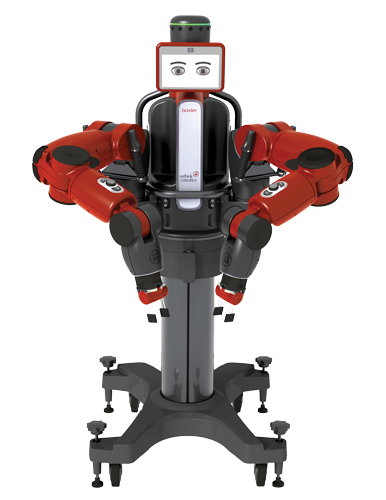
\includegraphics[width=0.4\linewidth]{baxter1.png}}
	\caption{Робот Baxter}
	\label{img:baxter}
\end{figure}

Отличительной особенностью этих роботов является изменение их конфигурации под нужные технологические процессы происходит в виде <<обучения>> в специальном графическом приложении Intera Studio~\ref{img:intera}, а не классического программирования промышленных роботов. Особенностью технологий Rethink Robotics являются роботы, которые экономически эффективны и могут работать совместно с коллегами-людьми, выполняя, например, опасные для людей работы. 

\begin{figure}[h!]
	\centering{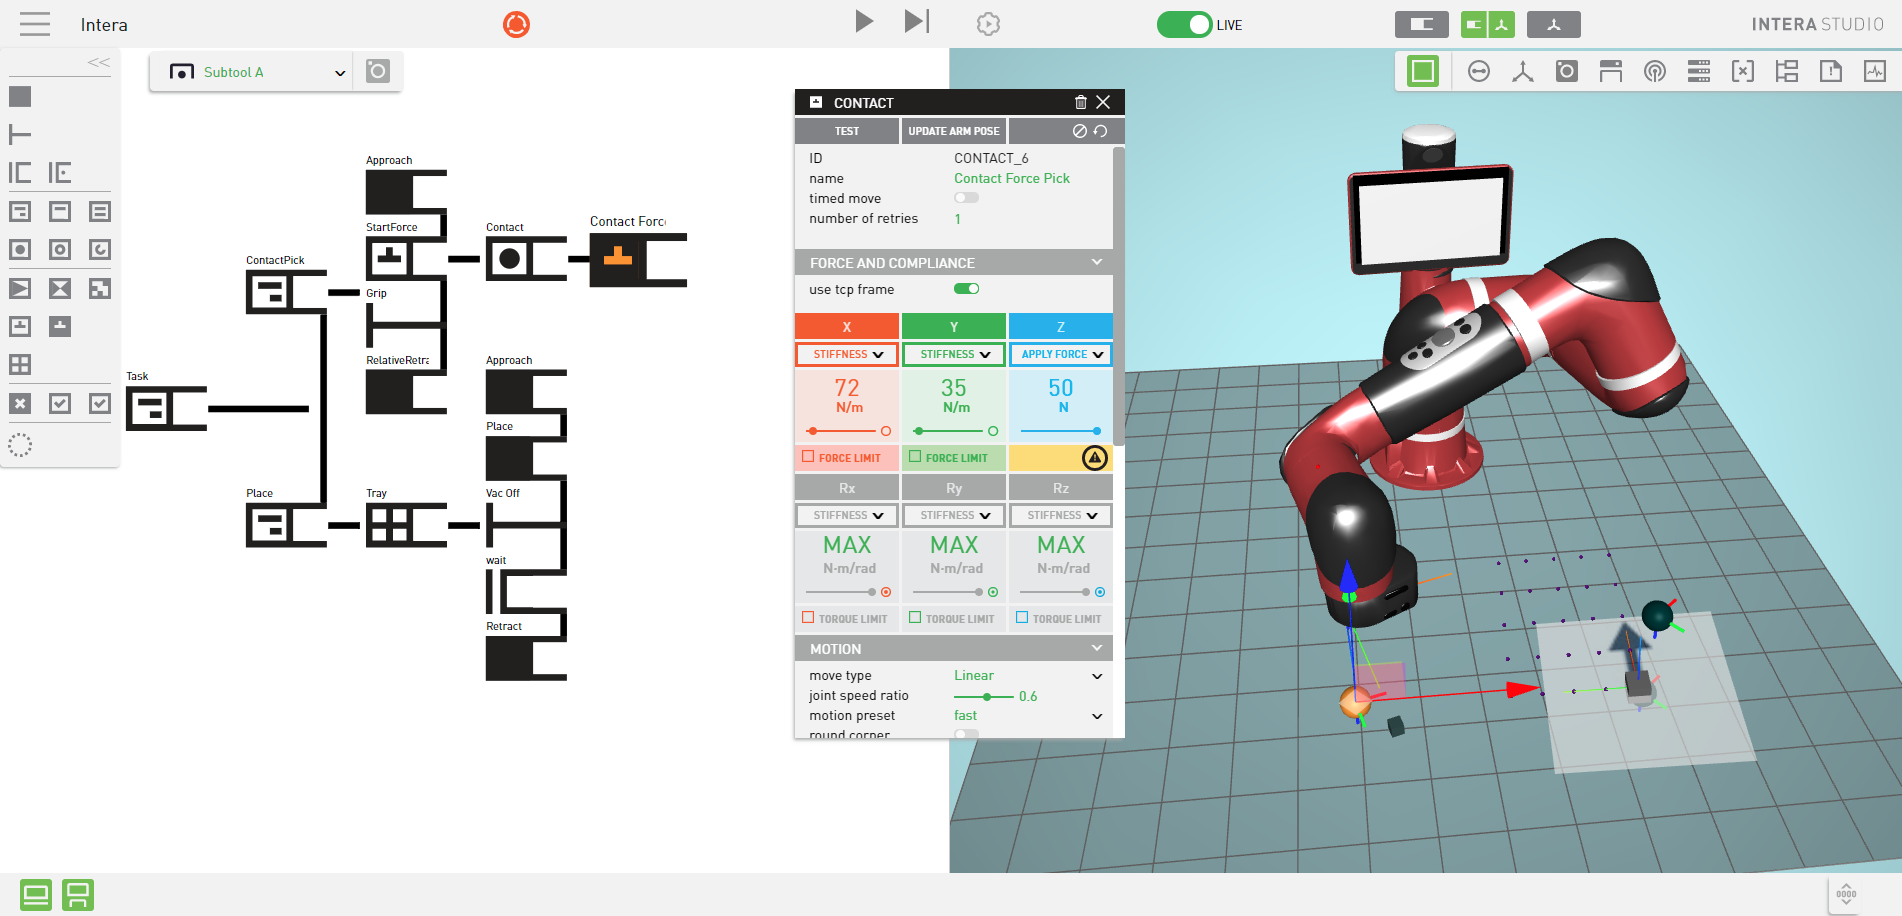
\includegraphics[width=1\linewidth]{intera.png}}
	\caption{Окно приложения Intera Studio для программирования роботов компании Rethink Robotics}
	\label{img:intera}
\end{figure}

По периметру <<головы>> робота располагаются датчики, которые дают возможность ему адаптироваться к окружающей среде, определять наличие людей рядом. В <<руках>> робота установлены инфракрасные датчики. Доступно большое разнообразие схватов.

Многие университеты используют робота Baxter в рамках своих курсов по робототехнике~\cite{baxteruse}, чтобы дать студентам возможность использования современной технологии робототехники для практического применения в реальном мире. Baxter, в отличие от традиционных роботов-манипуляторов, не требует установки вокруг себя заграждений, поэтому студенты могут работать с ним в непосредственной близости, не беспокоясь о безопасности.
% http://www.rethinkrobotics.com/

%%%%%%%%%%%%%%%%%%%%
%%% Robotnik RB-1
\textit{Robotnik}~--- испанская компания, специализирующаяся на разработке роботов и R\&D в области робототехники. Один из их роботов RB-1, это модульный мобильный манипулятор, разработанный с возможностью расширения. Применяется  для R\&D, AAL (Ambient Assisted Living) и удаленного управления. Изображение робота показано на рисунке~\ref{img:rb1}.

\begin{figure}[h!]
	\centering{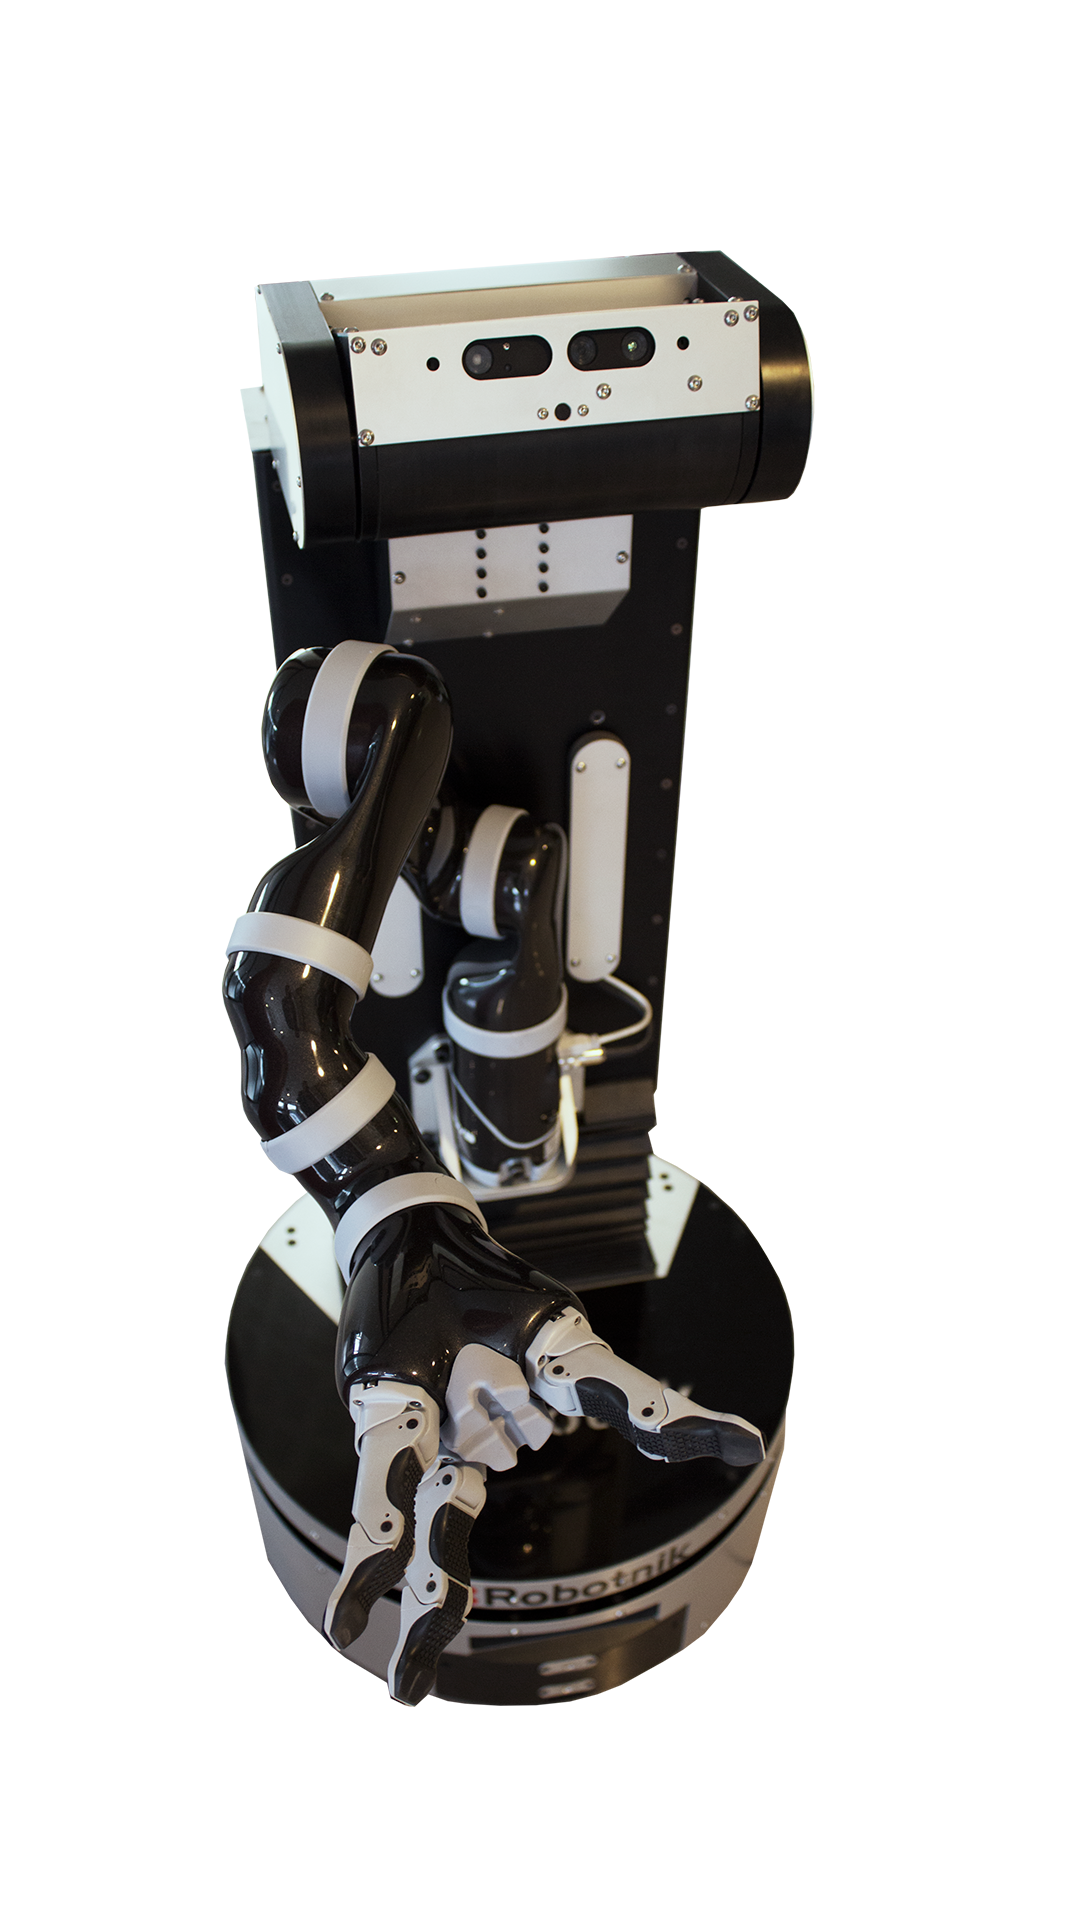
\includegraphics[width=0.30\linewidth]{rb1.png}}
	\caption{Робот испанской компании Robotnik RB-1}
	\label{img:rb1}
\end{figure}

Манипулятор имеет антропоморфную конфигурацию с семью степенями свободы и двух или трехпальцевый захват. Что касается датчиков, в мобильной платформе RB-1 установлен лидар Hokuyo URG-04LX-UG01, для задач навигации и система компьютерного зрения с одной из RGBD камер Microsoft Kinect или  ASUS Xtion PRO Live.

Программное обеспечения с открытыми исходными кодами, управление реализуется посредством ROS (Robotic Operation System). Компания поставляет роботов в нескольких модификациях~\cite{review}.
% https://www.robotnik.eu/manipulators/rb-one/


%%%%%%%%%%%%%%%%%%%%
%%% PAL Robotics TIAGO 
\textit{PAL Robotics}~--- испанская команда вдохновленных инженеров, которые разрабатывают, изготавливают и модифицируют роботов. Их робот TIAGo (Take It And Go)~--- мобильная исследовательская платформа, предназначенная для навигации, манипуляции и взаимодействия с окружающим миром. Оснащена дифференциальной платформой. 

Робот включает в себя систему технического зрения, подъемный торс и манипулятор, обеспечивающие большое рабочее пространство. Полностью совместим с ROS и, кроме того, поставляется с множеством готовых функциональных возможностей, таких как: мультисенсорная навигация, планирование движения без конфликтов, обнаружение людей, лиц и объектов, распознавание речи и синтез. Общий вид робота представлен на рисунке~\ref{img:tiago}~\cite{review}.

\begin{figure}[h!]
	\centering{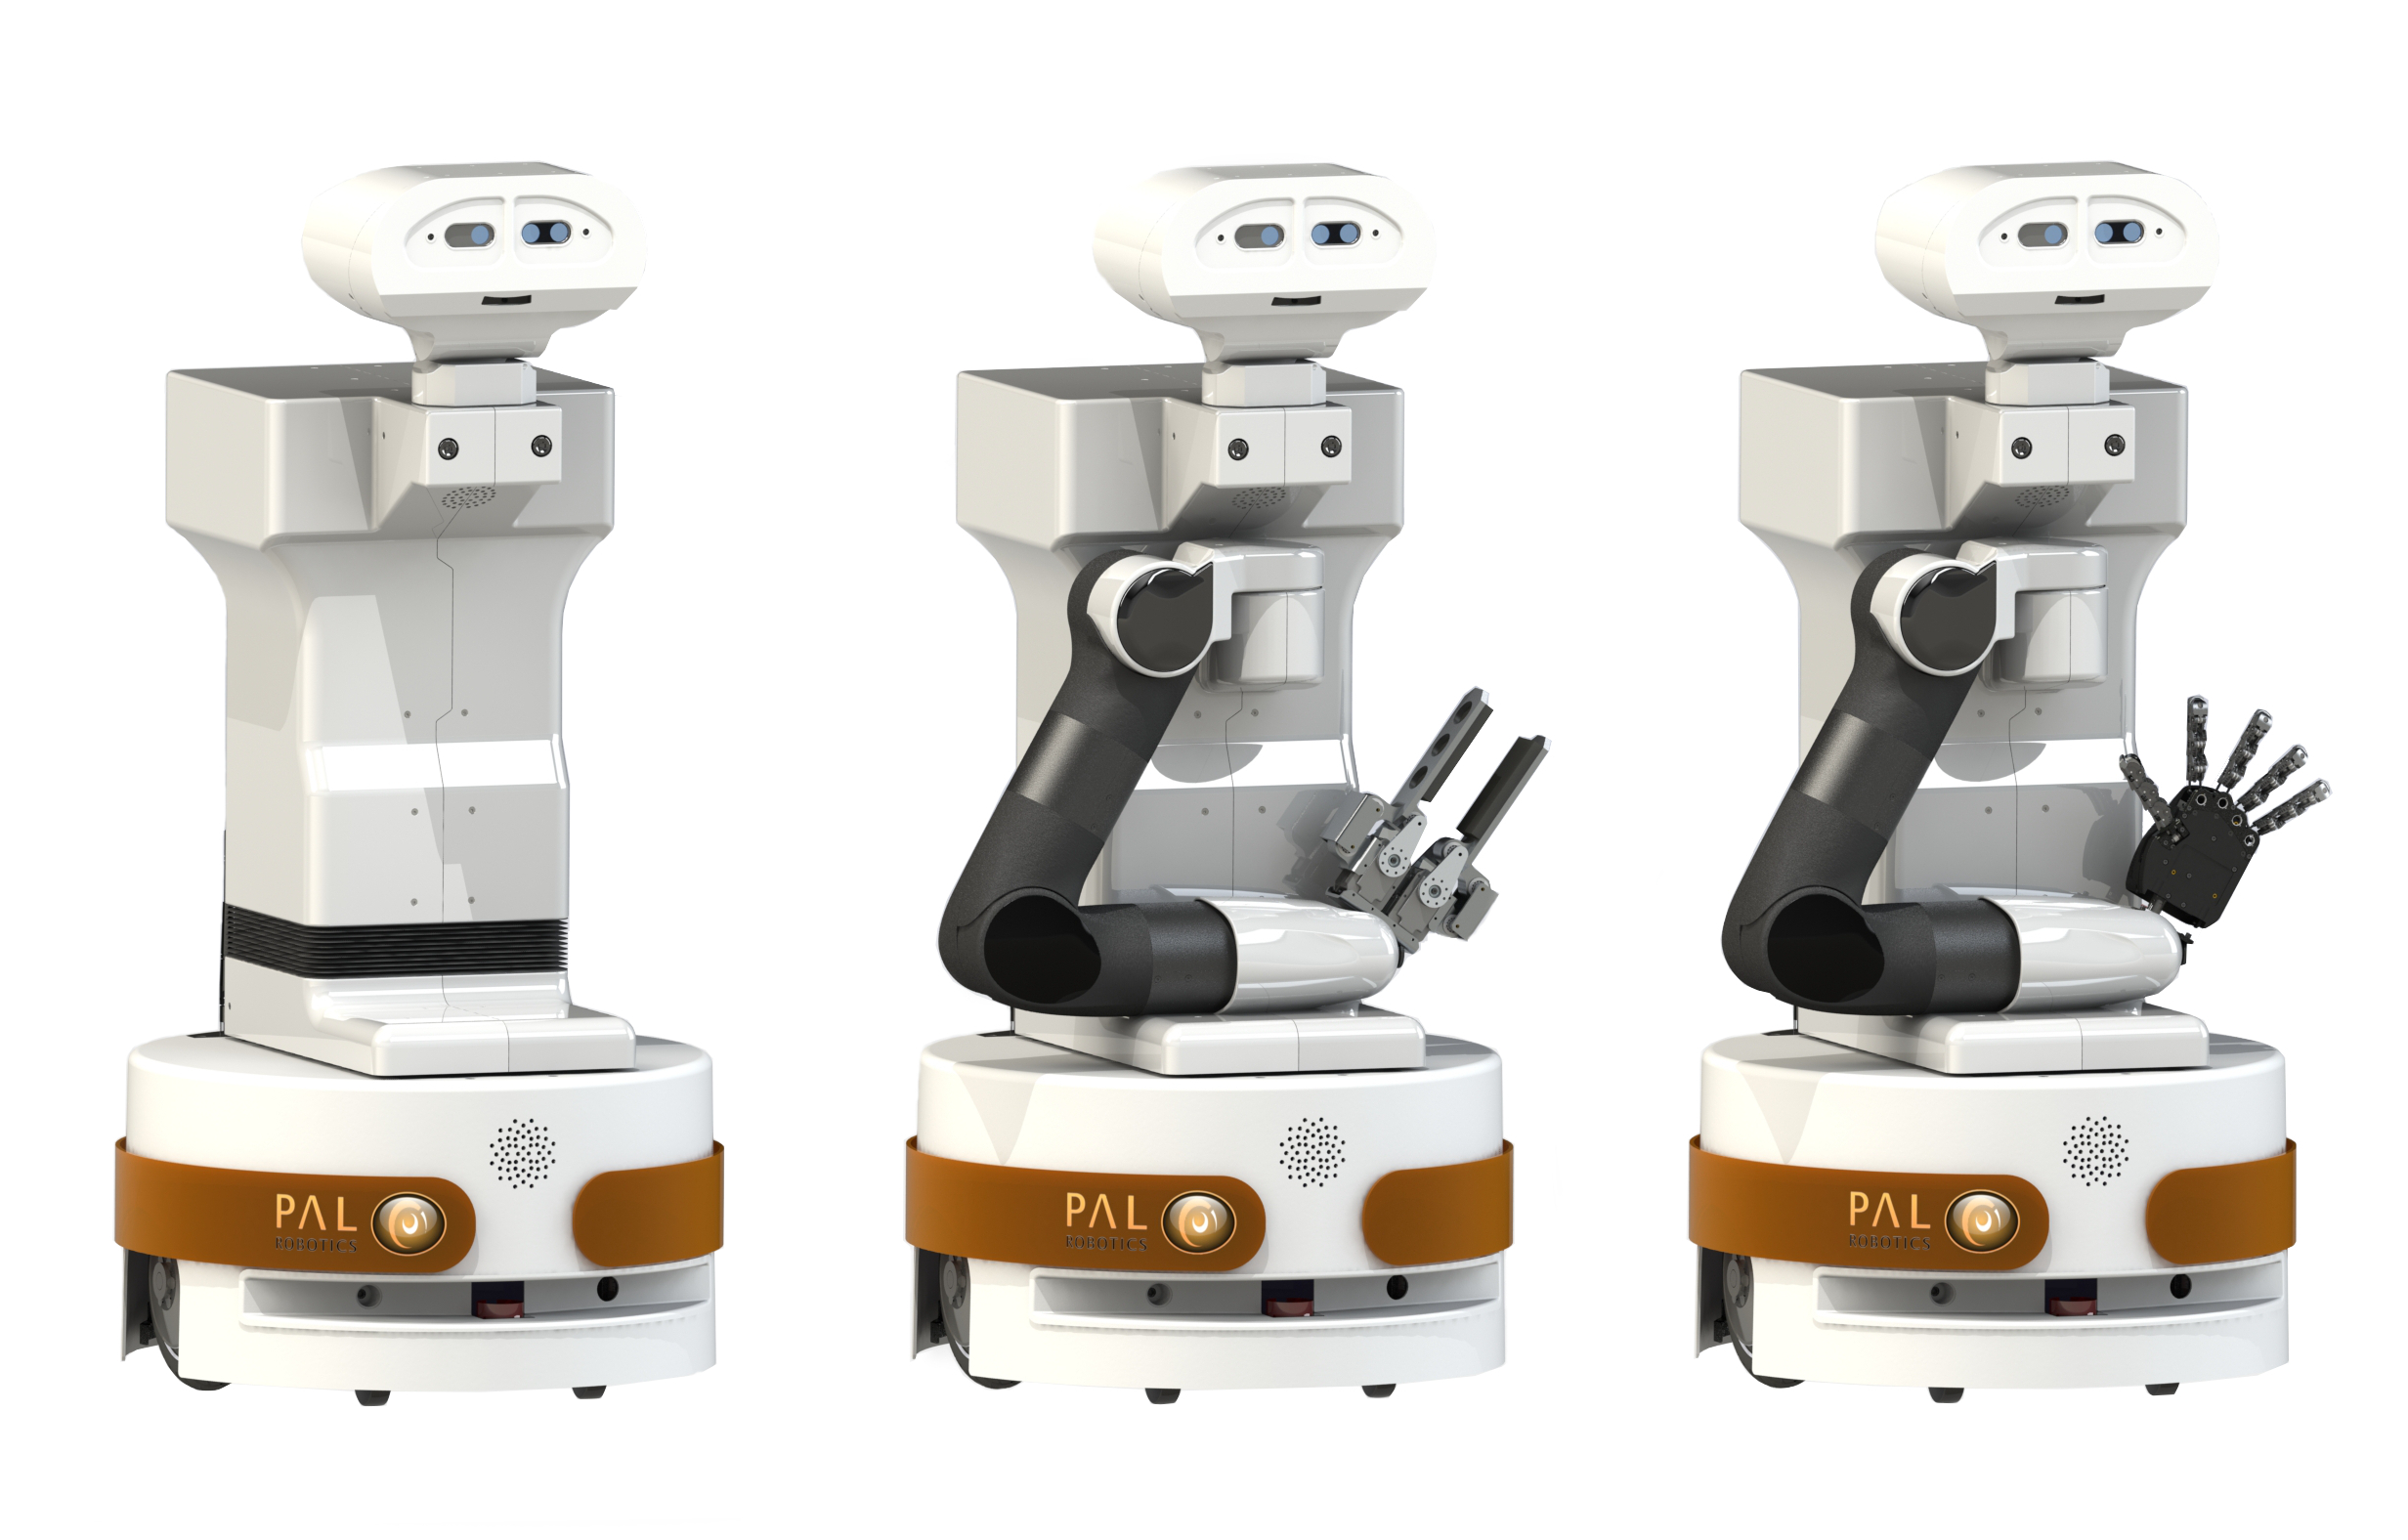
\includegraphics[width=0.9\linewidth]{tiago.jpg}}
	\caption{Робот испанской компании PAL Robotics TIAGO}
	\label{img:tiago}
\end{figure}


%%%%%%%%%%%%%%%%%%%%
%%% Care-O-bot 4 
\textit{Fraunhofer IPA}~--- немецкая компания, выпускающая целую линейку роботов, для исследований. Один из них Care-O-bot 4, изображение которого представлено на рисунке~\ref{img:careobot}.

\begin{figure}[h!]
	\centering{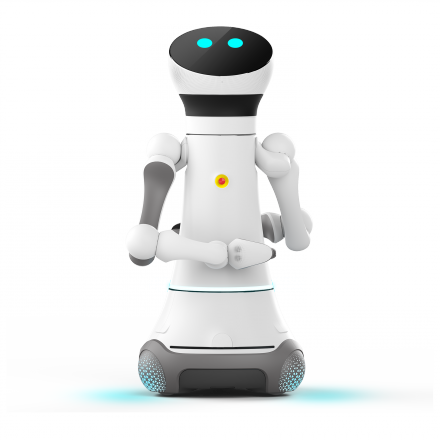
\includegraphics[width=0.5\linewidth]{careobot.png}}
	\caption{Робот немецкой компании Fraunhofer IPA Care-O-bot 4}
	\label{img:careobot}
\end{figure}

Самое интересное в Care-O-bot 4 (кроме двух рук и изысканных движений)~--- его модульность. Робот состоит из пяти модулей: основание, туловище, руки, кольцо датчиков и голова. Каждый из модулей может быть отсоединён, в зависимости от задач.

Робот может найти применение как дома, в качестве повседневного помощника, так и в муниципальных учреждениях для оказания различных услуг~\cite{review}.
% http://www.mojin-robotics.de/

\textit{Moley Robotics}~--- это робототехническая компания, основанная Марком Олейник в 2015 году для создания сервисных роботов для использования на кухне. Прототип робота Moley Robotic Kitchen~--- это роботизированная кухня. Изображение прототипа показано на рисунке~\ref{img:moley}

\begin{figure}[h!]
	\centering{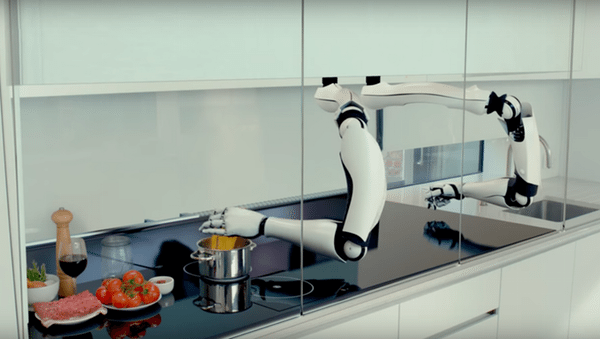
\includegraphics[width=0.9\linewidth]{moley2.png}}
	\caption{Робот компании Moley Robotic Kitchen}
	\label{img:moley}
\end{figure}

Moley Robotic Kitchen включает в себя два манипулятора со схватами в виде кистей рук, оснащенные тактильными датчиками, кухонный стол с духовкой, электрической плитой, посудомоечной машиной и сенсорным экраном. Манипуляторы могут захватывать и взаимодействовать с большинством кухонных принадлежностей~\cite{moley}.

Робот умеет запоминать движения человека, когда тот готовит некоторое блюдо и затем, воспроизводить их при приготовлении того же блюда самостоятельно.

В текущем прототипе пользователь управляет установкой с помощью встроенного сенсорного экрана или приложения для смартфона с готовыми ингредиентами, приготовленными заранее и помещенными в определенные места. Целью Moley Robotic в будущем является предоставление пользователю возможности выбирать из библиотеки более 2000 записанных рецептов.

Исследовательский робот немецкой компании \textit{KUKA} YouBot~--- образовательный робот, специально разработанный для разработки и обучения в области мобильных манипуляторов. Он состоит из омни-платформы, пятистепенного манипулятора и двухпальцевого схвата. KUKA YouBot~--- это платформа с открытым исходным кодом, представлена на рисунке~\ref{img:ky}.

\begin{figure}[h!]
	\centering{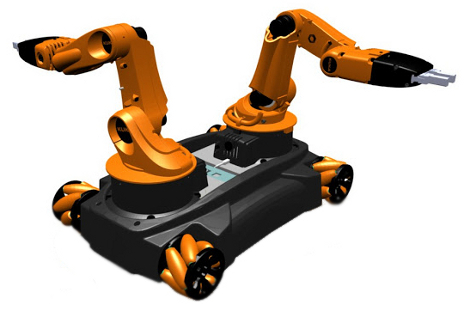
\includegraphics[width=0.8\linewidth]{ky.jpg}}
	\caption{Робот компании KUKA YouBot}
	\label{img:ky}
\end{figure}

\newpage
\section{Разработка системы управления манипулятором KUKA YouBot}\label{part_manipulator}

Раздел посвящён теоретическим выкладкам, позволяющим схвату манипулятора перемещаться по заданной траектории. Сначала определяются основные кинематические соотношения, описывающие манипулятор KUKA YouBot (далее манипулятор) без учета действующих на него сил. Они позволяют определить положение манипуляционного механизма в пространстве, а также скорости и ускорения всех звеньев. Синтезируется система управления с использованием кинематических соотношений.

%Во второй части исследуются алгоритмы динамического управления, учитывающие динамику манипулятора при определении управляющих воздействий. Получается динамическая модель манипулятора в форме уравнений Лагранжа, которая представляется в \textcolor{red}{матричной форме для реализации системы управления} и регрессионной для проведения процедуры идентификации динамических параметром манипулятора. Синтезируется система моментного управления.

\subsection{Описание манипулятора}\label{section_description_of_robot}
Основной элемент практически любого робота это~--- манипулятор, в этой работе представленный манипулятором с робота KUKA Youbot и изображённый на рисунке~\ref{img:sizes_of_robot}в. Его механизм имеет пять степеней подвижности. Многозвенная конструкция манипулятора заканчивается двухпальцевым схватом ~--- инструментом, предназначенным для захвата объектов определённой формы.	

Описание технических характеристик дается таблицей~\ref{table_gen_info_of_manipulator} и рисунком~\ref{img:sizes_of_robot}.
%Неуказанные там параметры робота, требуемые для дальнейших расчетов, неизвестны и поэтому подлежат измерению или идентификации, речь о которых пойдет ниже по тексту.

\begin{table}[h!]
	\caption{Общая информация о манипуляторе робота Kuka Youbot.}
	\begin{center}
		\begin{tabularx}{1\textwidth}{|>{\hsize=0.7\textwidth}X|Y|}
			\hline
			\multicolumn{1}{|c|}{Параметр} & \makebox[3cm]{Значение}\\
			\hline
			Количество сочленений & 5\\
			\hline
			Объем рабочей области, $ \text{м}^2 $ & 0.513 \\
			\hline
			Масса, $ \text{кг} $ & 5.3\\
			\hline
			Допустимая нагрузка, $ \text{кг} $ & $0.5$~\\
			\hline
			Точность повторного воспроизведения позиции, $ \text{мм} $ & 1\\
			\hline
			Максимальная скорость в сочленении, $ ^\circ\text{ с}^{-1} $& $90$\\
	    	\hline
			Интерфейс & EtherCAT\\
			\hline
			Напряжение питания, $ \text{В} $ & 24\\
			\hline
		\end{tabularx}
	\end{center}
	\label{table_gen_info_of_manipulator}
\end{table}

\begin{figure}[p]
	\center{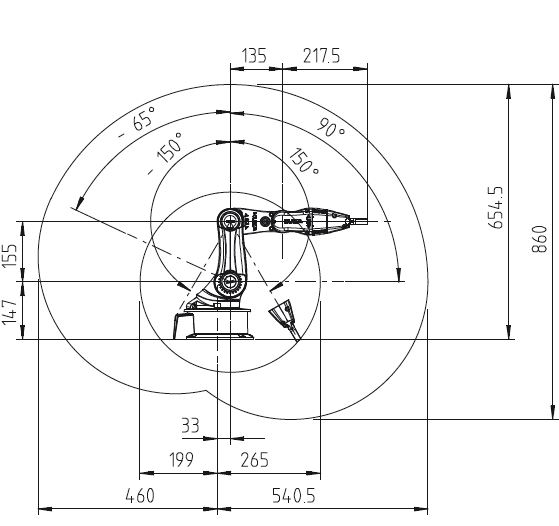
\includegraphics[width=0.7\textwidth]{youbot_workspace_1.jpg} \\ а)}
	\vfill
	\begin{minipage}[h]{0.47\linewidth}
		\centering{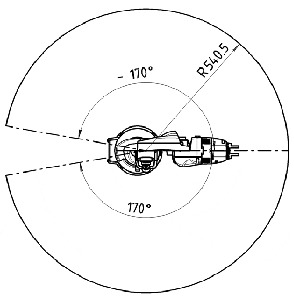
\includegraphics[width=0.95\linewidth]{youbot_workspace_2.jpg} \\ б)}
	\end{minipage}
	\hfill
	\begin{minipage}[h]{0.47\linewidth}
		\centering{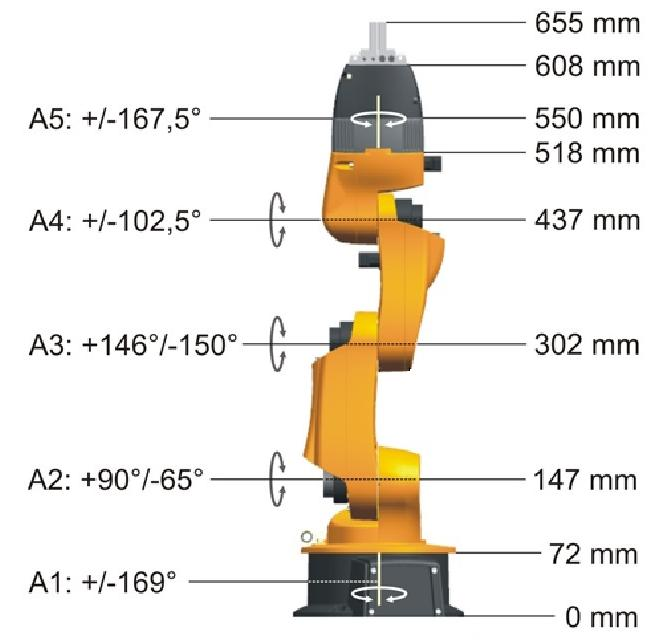
\includegraphics[width=0.95\linewidth]{youbot_length.jpg} \\ в)}
	\end{minipage}
	\caption{Некоторые параметры манипулятора Kuka Youbot: a~--- размеры рабочей области (вид сбоку); б~--- размеры рабочей области (вид сверху); в~--- длины звеньев и предельные значения для углов вращения по каждому из сочленений~\cite{youbot_detailed_specifications}.}
	\label{img:sizes_of_robot}
\end{figure}

%		\hline
%		Поворот 1 сочленения &  $ \pm 169^\circ $\\
%		\hline
%		Поворот 2 сочленения &  $ +90^\circ / -65^\circ$\\
%		\hline
%		Поворот 3 сочленения &  $ +146^\circ / -151^\circ$\\
%		\hline
%		Поворот 4 сочленения &  $\pm 102,5^\circ$\\
%		\hline
%		Поворот 5 сочленения &  $\pm 167,5^\circ$\\
\newpage
\subsection{Кинематическая модель манипулятора}\label{part_kinematic_model}
\subsubsection{Решение задач о положении манипулятора}\label{part_kinematic_position}
Планирование траектории движения схвата манипулятора предполагает определение соотношений между координатами схвата, заданными в различной форме: обобщенными координатами самого манипулятора и шестью числами, задающими положение и ориентацию схвата в связанной с ним системе координат.

Последовательная кинематическая цепь рассматриваемого манипулятора, включающая только вращательные кинематические пары (КП) V-класса (цилиндрические шарниры), изображена на рисунке~\ref{img:kinematics}a.

\begin{figure}[h!]
	\begin{minipage}[h]{0.5\linewidth}
		\centering{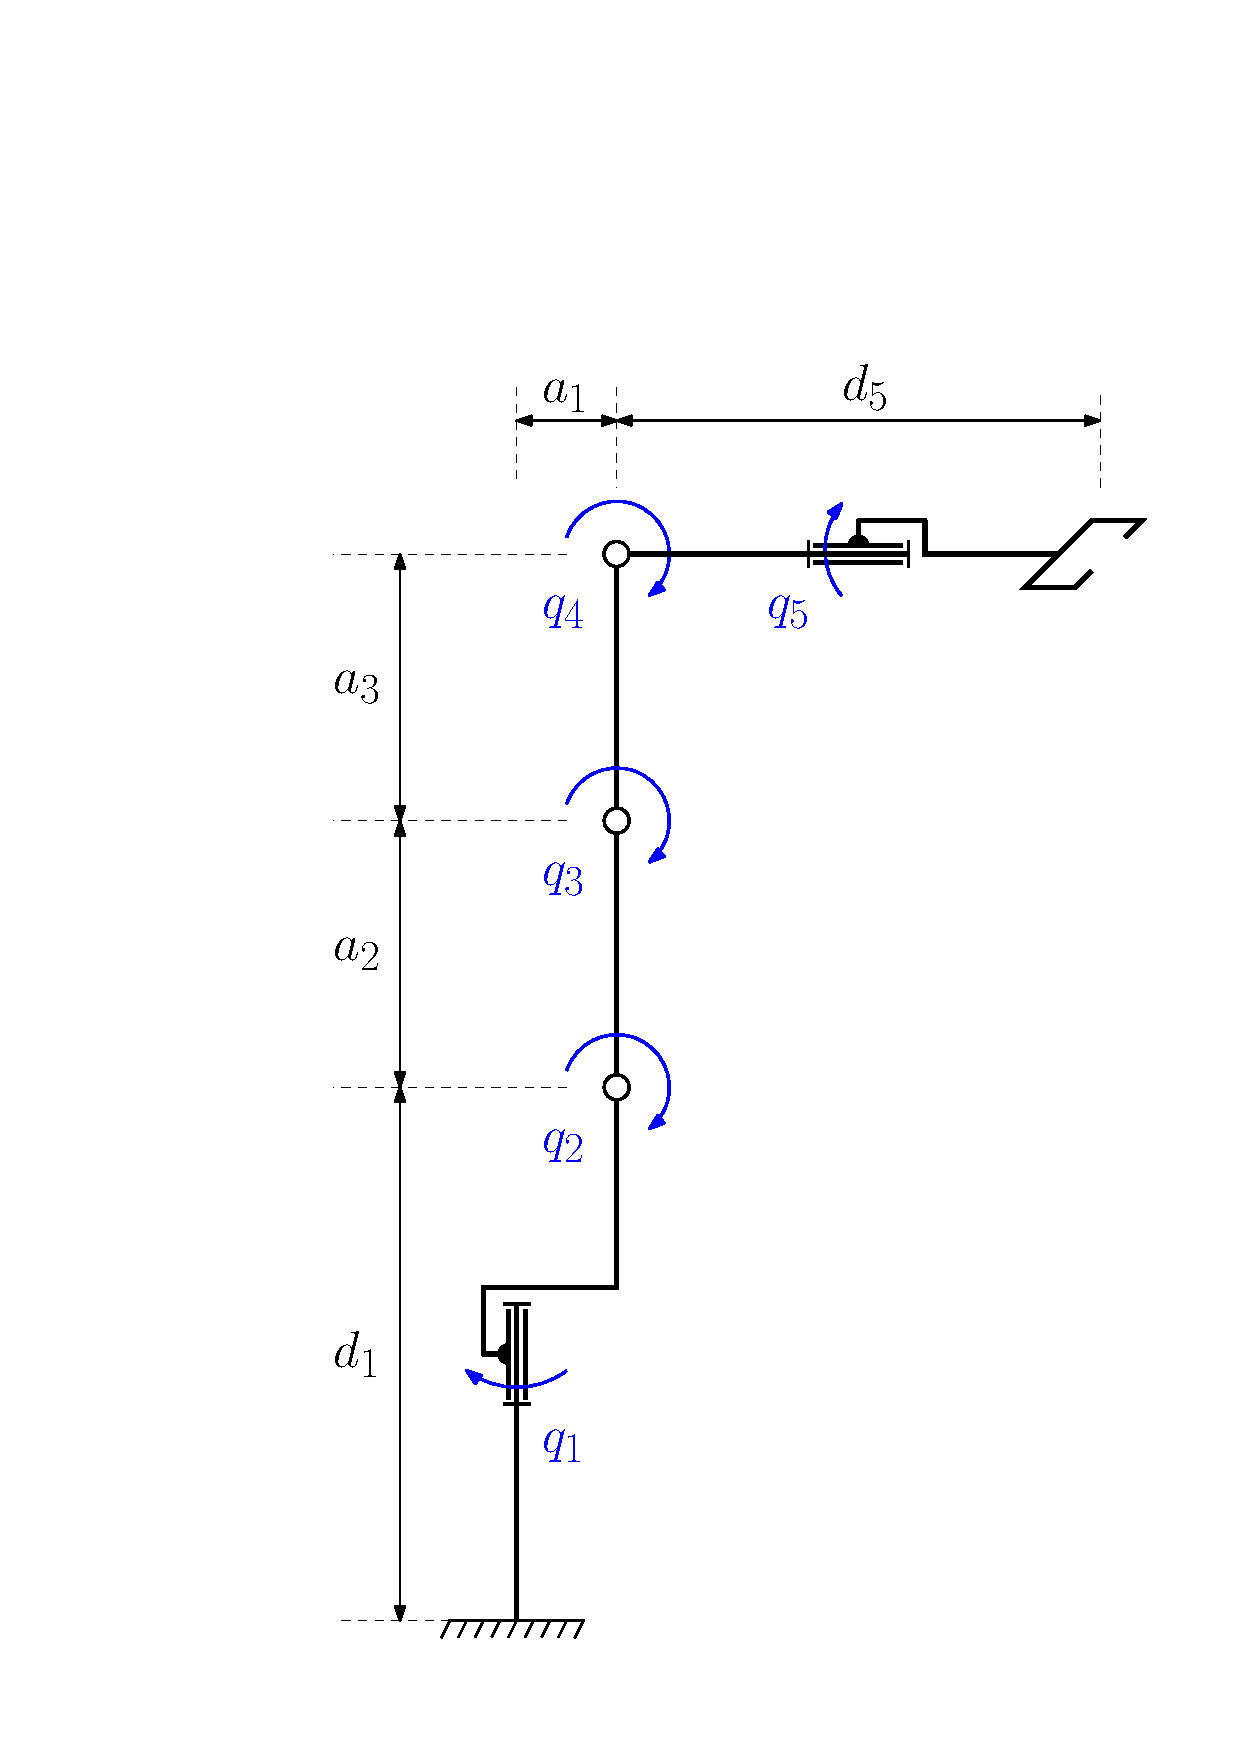
\includegraphics[width=0.95\linewidth]{kinematics_schema.pdf} \\ а)}
	\end{minipage}
	\hfill
	\begin{minipage}[h]{0.5\linewidth}
		\centering{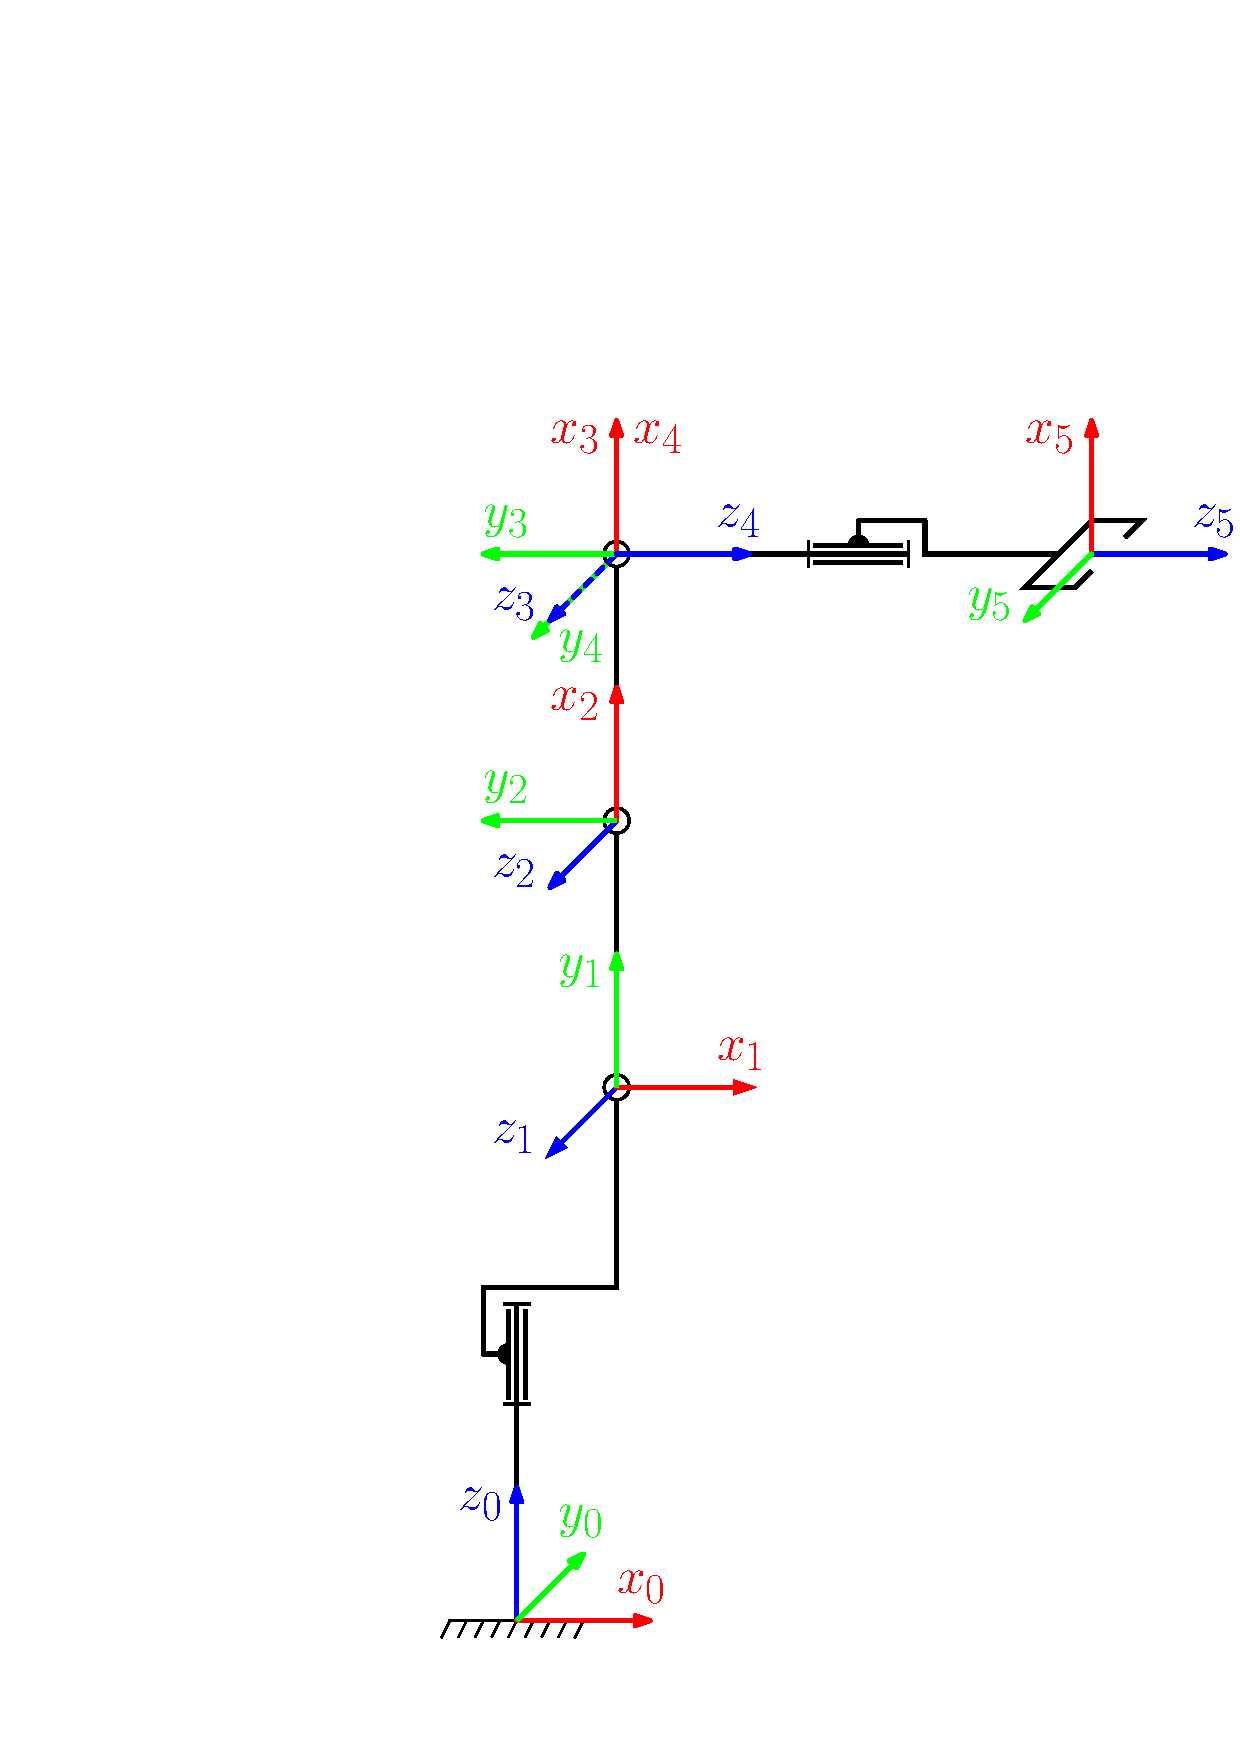
\includegraphics[width=0.95\linewidth]{kinematics_frames.pdf} \\ б)}
	\end{minipage}
	\caption{Схемы рассматриваемого манипулятора: а~--- кинематическая при $\theta=\left[\theta_1,\,\theta_2,\,\theta_3,\,\theta_4,\,\theta_5\right]^T = \left[0,\,\pi/2,\,0,\,0,\,0\right]^T$; б~--- расположения СК КП.}
	\label{img:kinematics}
\end{figure}

Процедура описания положений звеньев манипулятора друг относительно друга в соответствии с методом Денавита-Хартенберга \cite{spong2005robot}, представляется тремя шагами:
\begin{enumerate}
    \item <<привязка>> к каждому звену СК, чьи оси удовлетворяют следующим условиям:
    \begin{enumerate}
	    \item ось $z_{i-1}$ направлена вдоль оси $i$-ой КП;
        \item ось $x_i$ перпендикулярна оси $z_{i-1}$ и пересекает ее;
        \item ось $y_i$ дополняет оси $z_i$ и $x_i$ до правой декартовой СК.
    \end{enumerate}
    \item определение параметров ДХ:
    \begin{enumerate}
	    \item $a_i$~--- расстояния от $z_{i-1}$ до $z_i$ вдоль $x_i$;
	    \item $\alpha_i$~--- угла от $z_{i-1}$ до $z_i$ вокруг $x_i$;
        \item $d_i$~--- расстояния от $x_{i-1}$ до $x_i$ вдоль $z_{i-1}$;
        \item $\theta_i$~--- угла от $x_{i-1}$ до $x_i$ вокруг $z_{i-1}$.
    \end{enumerate}
    \item расчет матриц однородного преобразования в соответствии со следующими формулами:
    \begin{equation}\label{DH_matrix}
        {}^{i-1}A_{i} = R_{z, \theta_i} \cdot T_{z, d_i} \cdot T_{x, a_i} \cdot R_{x, \alpha_i}
    \end{equation}
    где $R_{z, \theta_i}$~--- матрица поворота вокруг оси $z$ на угол $\theta_i$, $T_{z, d_i}$~--- матрица смещения вдоль оси $z$ на расстояние $d$, $T_{x, a_i}$~---матрица смещения вдоль оси $x$ на расстояние $a_i$,  $R_{x, \alpha_i}$~--- матрица поворота вокруг оси $x$ на угол $\alpha_i$, равные
    \begin{gather}
        R_{z, \theta_i} =
        \begin{bmatrix}
            \cos\theta_i & -\sin\theta_i & 0 & 0\\
            \sin\theta_i &  \cos\theta_i & 0 & 0\\
            0 & 0 & 1 & 0\\
            0 & 0 & 0 & 1
        \end{bmatrix}\!\!,
        \quad
        T_{z, d_i} =
        \begin{bmatrix}
            1 & 0 & 0 & 0\\
            0 & 1 & 0 & 0\\
            0 & 0 & 1 & d_i\\
            0 & 0 & 0 & 1\\
        \end{bmatrix}\!\!,\\
\end{gather}
\begin{gather}   %
        T_{x, a_i} =
        \begin{bmatrix}
            1 & 0 & 0 & a_i\\
            0 & 1 & 0 & 0\\
            0 & 0 & 1 & 0\\
            0 & 0 & 0 & 1\\
        \end{bmatrix}\!\!,
        \quad
        R_{x, \alpha_i} =
        \begin{bmatrix}
            1 & 0 & 0 & 0\\
            0 & \cos\alpha_i & -\sin\alpha_i & 0\\
            0 & \sin\alpha_i &  \cos\alpha_i & 0\\
            0 & 0 & 0 & 1
        \end{bmatrix}\!\!;
    \end{gather}
    итого
    \begin{equation}
        {}^{i-1}A_i =
        \begin{bmatrix}
            \cos\theta_i & - \cos\alpha_i \sin\theta_i & \sin\alpha_i \sin\theta_i & a_{i} \cos\theta_i\\
            \sin\theta_i & \cos\alpha_i \cos\theta_i & - \sin\alpha_i \cos\theta_i & a_{i} \sin\theta_i\\
            0 & \sin\alpha_i & \cos\alpha_i & d_{i}\\
            0 & 0 & 0 & 1
        \end{bmatrix}
    \end{equation}
\end{enumerate}

Результаты выполнения двух первых шагов для исследуемого манипулятора представлены на рисунке~\ref{img:kinematics}б и в таблице~\ref{table_DH_params}, а третьего~--- в лице следующих выражений:
\begin{gather}\label{eq_all_ht_matrices}
	{}^0A_1\! =\!\!
    \left[\begin{matrix}c_1 & 0 & s_1 & a_{1} c_1\\s_1 & 0 & - c_1 & a_{1} s_1\\0 & 1 & 0 & d_{1}\\0 & 0 & 0 & 1\end{matrix}\right]\!\!;
    %
	{}^1A_2\! =\!\!
	\left[\begin{matrix}c_2 & - s_2 & 0 & a_{2} c_2\\s_2 & c_2 & 0 & a_{2} s_2\\0 & 0 & 1 & 0\\0 & 0 & 0 & 1\end{matrix}\right]\!\!;
    %
	{}^2A_3\! =\!\!
	\left[\begin{matrix}c_3 & - s_3 & 0 & a_{3} c_3\\s_3 & c_3 & 0 & a_{3} s_3\\0 & 0 & 1 & 0\\0 & 0 & 0 & 1\end{matrix}\right]\!\!;\notag
	\\
	{}^3A_4 =
	 \left[\begin{matrix}c_4 & 0 & s_4 & 0\\s_4 & 0 & - c_4 & 0\\0 & 1 & 0 & 0\\0 & 0 & 0 & 1\end{matrix}\right]\!\!;
	\;
	{}^4A_5 =
	\left[\begin{matrix}c_5 & - s_5 & 0 & 0\\s_5 & c_5 & 0 & 0\\0 & 0 & 1 & d_{5}\\0 & 0 & 0 & 1\end{matrix}\right]\!\!\ldotp
\end{gather}

\textbf{Прямая задача кинематики}\label{part_kinematics_forward} решается из  соотношений, содержащихся в информации о смещении и повороте СК $Ox_5y_5z_5$ относительно СК $Ox_0y_0z_0$, содержащейся в матрице ${}^0A_5$.
Следовательно, чтобы решить ПЗК, необходимо найти эту матрицу в соответствии c выражением:
\begin{equation}\label{fk}
	{}^0A_5 = \prod^{5}_{i=1}{{}^{i-1}A_i(q_i)}\ldotp
\end{equation}

\begin{table}[h!]
	\caption{Параметры Денавита-Хартенберга}
	\begin{center}
		\begin{tabularx}{1\textwidth}{|>{\hsize=0.15\textwidth}Y|>{\hsize=0.15\textwidth}Y|>{\hsize=0.15\textwidth}Y|>{\hsize=0.15\textwidth}Y|Y|}
			\hline
			Звено, $i$ 	& $a_i$, мм & $\alpha_i$, рад & $d_i$, мм & $\theta_i$, рад\\
			\hline
			1  		& $33$ & $\pi/2$ & $147$ & \parbox[c][0.7\height]{4cm}{$$\pi \cdot \cfrac{169^\circ}{180^\circ} - q_1$$}\\
			\hline
			2 		& $155$ & $0$ 	& $0$ & \parbox[c][0.7\height]{4cm}{$$\pi \cdot \cfrac{65^\circ}{180^\circ} + \cfrac{\pi}{2} - q_2$$}\\
			\hline
			3 		& $135$ & $0$ 	& $0$ 	& \parbox[c][0.7\height]{4cm}{$$-\pi \cdot \cfrac{146^\circ}{180^\circ} - q_3$$}\\
			\hline
			4 	& $0$ & $\pi/2$ & $0$ & \parbox[c][0.7\height]{4cm}{$$\pi \cdot \cfrac{102.5^\circ}{180^\circ} + \cfrac{\pi}{2} - q_4$$}\\
			\hline
			5 		& $0$ & $0$ 	& $218$     & \parbox[c][0.7\height]{4cm}{$$\pi \cdot \cfrac{167.5^\circ}{180^\circ} - q_5$$}\\
			\hline
		\end{tabularx}
	\end{center}
	\label{table_DH_params}
\end{table}

Решая \textbf{обратную задачу кинематики}\label{part_kinematics_inverse}, найдём соотношения для положений сочленений при известном положении и ориентации схвата. Заданные смещение и поворот СК $Ox_5y_5z_5$ относительно СК $Ox_0y_0z_0$ можно описать с помощью матрицы ${}^0A_5$.
Используя ее и матрицы из~\eqref{eq_all_ht_matrices}, найти расчетные формулы для углов $q_i$ ($i=\overline{1,5}$) можно из следующих соображений~\cite{craig2018introduction}.

Для неизвестной матрицы ${}^0A_5$ вводятся следующие обозначения ее элементов:
\begin{equation}\label{ik}
	{}^0A_5 =
	\left[\begin{matrix}
	r_{11} & r_{12} & r_{13} & p_{x}\\
	r_{21} & r_{22} & r_{23} & p_{y}\\
	r_{31} & r_{32} & r_{33} & p_{z}\\
	0 & 0 & 0 & 1
	\end{matrix}\right]\!\!\ldotp
\end{equation}

Далее, составляется равенство из матрицы ${}^0A_5$ и правой части выражения~\eqref{fk}, затем полученное равенство с обеих сторон умножается на ${}^0A_1^{-1}$:
\begin{equation}
	{}^0A_1^{-1} \cdot {}^0A_5 = {}^1A_2 \cdot {}^2A_3 \cdot {}^3A_4 \cdot {}^4A_5,
\end{equation}
где левая часть с учетом~\eqref{eq_all_ht_matrices} равна
\begin{equation}\label{eq_left_part}
	{}^0A_1^{-1} \cdot {}^0A_5 =
	\left[\begin{matrix}
		r_{11} c_{1} + r_{21} s_{1} & r_{12} c_{1} + r_{22} s_{1} & r_{13} c_{1} + r_{23} s_{1} &  p_{x} c_{1} + p_{y} s_{1} - a_{1}\\
		r_{31} & r_{32} & r_{33} & p_{z} - d_{1}\\
		r_{11} s_{1} - r_{21} c_{1} & r_{12} s_{1} - r_{22} c_{1} & r_{13} s_{1} - r_{23} c_{1} & p_{x} s_{1} - p_{y} c_{1}\\
		0 & 0 & 0 & 1\end{matrix}\right]\!\!,
\end{equation}
а правая
\begin{equation}\label{eq_right_part}
	{}^1A_2 \cdot {}^2A_3 \cdot {}^3A_4 \cdot {}^4A_5 =
	\left[\begin{matrix}
		c_{5} c_{234} & - s_{5} c_{234} & s_{234} & a_{2} c_{2} + a_{3} c_{23} + d_{5} s_{234}\\
		c_{5} s_{234} & - s_{5} s_{234} & - c_{234} & a_{2} s_{2} + a_{3} s_{23} - d_{5} c_{234}\\
		s_{5} & c_{5} & 0 & 0\\
		0 & 0 & 0 & 1
	\end{matrix}\right]\!\!,
\end{equation}
где, в свою очередь,
\begin{equation}\label{eq_theta_23_234}
    \theta_{23} = \theta_2 + \theta_3,
    \qquad
    \theta_{234} = \theta_2 + \theta_3 + \theta_4\ldotp
\end{equation}

Теперь, решая уравнения, полученные из равенства матриц~\eqref{eq_left_part} и \eqref{eq_right_part}, выводятся выражения для углов $\theta_1$, $\theta_5$ и $\theta_{234}$

\begin{itemize}
    \item равенство элементов $(3,4)$:
        \begin{equation}\label{eq_for_theta_1}
	        p_{x} s_{1} - p_{y} c_{1} = 0
            \; \Rightarrow \;
	        \tg \theta_1 = \cfrac{p_y}{p_x}
	        \; \Rightarrow \;
	        \left\{
	        \begin{aligned}
		        \!&\theta_1^\msf{I} = \atan2(p_y, p_x)\\
		        \!&\theta_1^\msf{II} = \atan2(-p_y, -p_x)
            \end{aligned}
            \right.
        \end{equation}
    \item равенство элементов $(3,1)$ и $(3,2)$:
        \begin{multline}
            \left\{
	        \begin{aligned}
		        \!&s_{5} = r_{11} s_{1} - r_{21} c_{1}\\
		        \!&c_{5} = r_{12} s_{1} - r_{22} c_{1}
            \end{aligned}
            \right.
            \qquad \Rightarrow
            \\
            \Rightarrow \;
            \left\{
	        \begin{aligned}
		        \!&\theta_5^\msf{I} = \atan2(r_{11} \sin\theta_1^\msf{I} - r_{21} \cos\theta_1^\msf{I},\: r_{12} \sin\theta_1^\msf{I} - r_{22} \cos\theta_1^\msf{I})\\
		        \!&\theta_5^\msf{II} = \atan2(r_{11} \sin\theta_1^\msf{II} - r_{21} \cos\theta_1^\msf{II},\: r_{12} \sin\theta_1^\msf{II} - r_{22} \cos\theta_1^\msf{II})
            \end{aligned}
            \right.
        \end{multline}
    \item равенство элементов $(2,3)$ и $(1,3)$:
        \begin{multline}
            \left\{
	        \begin{aligned}
		        \!&c_{234} = -r_{33}\\
		        \!&s_{234} = r_{13} c_{1} + r_{23} s_{1}
            \end{aligned}
            \right.
            \qquad \Rightarrow
            \\
            \Rightarrow \qquad
            \left\{
	        \begin{aligned}
		        \!&\theta_{234}^\msf{I} = \atan2(r_{13} \cos\theta_1^\msf{I}  + r_{23} \sin\theta_1^\msf{I},\: -r_{33})\\
		        \!&\theta_{234}^\msf{II} = \atan2(r_{13} \cos\theta_1^\msf{II}  + r_{23} \sin\theta_1^\msf{II},\: -r_{33})
            \end{aligned}
            \right.
        \end{multline}
\end{itemize}

Домножая выражение~\eqref{eq_left_part} на ${}^4A_5^{-1}$ справа~--- получается матрица~${}^1A_4$:
\begin{equation}\label{eq_A14_matrix}
    {}^1A_4 =
    \begin{bmatrix}
        \cdots & \cdots & \cdots & (p_y - d_5 r_{23})s_1 + (p_x - d_5 r_{13})c_1 - a_1\\
        \cdots & \cdots & \cdots & p_z - d_1 - d_5 r_{33}\\
        \cdots & \cdots & \cdots & p_x s_1 - p_y c_1 - d_5(r_{13} s_1 - r_{23} c_1)\\
        0 & 0 & 0 & 1
    \end{bmatrix}\!\!,
\end{equation}
где $\cdots$~--- неинтересные элементы матрицы.

Нужно заметить, что c учетом~\eqref{eq_for_theta_1} и равенства элементов~$(3,3)$ в~\eqref{eq_left_part} и~\eqref{eq_right_part} справедливо
\begin{equation}
p_x s_1 - p_y c_1 - d_5(r_{13} s_1 - r_{23} c_1) = 0\ldotp
\end{equation}
С~учетом этого и~\eqref{eq_A14_matrix}:
\begin{equation}\label{eq_r_1_1_4}
    r^1_{1,\,4} =
    \begin{bmatrix}
        (p_y - d_5 r_{23})s_1 + (p_x - d_5 r_{13})c_1 - a_1 \\
        p_z - d_1 - d_5 r_{33} \\
        0
    \end{bmatrix}\!\!\ldotp
\end{equation}

Далее нужно заметить, что одно и то же положение 4-го звена может достигаться при двух разных способах расположения звеньев~2 и~3 (см.~рисунок~\ref{ik_geometric}).
Следовательно, углы $\theta_2$, $\theta_3$ и $\theta_4$ при одних и тех же значениях углов $\theta_1$ и $\theta_5$ имеют по два возможных значения. 
Ниже выводятся выражения для последних.

\begin{figure}[h!]
	\centering
	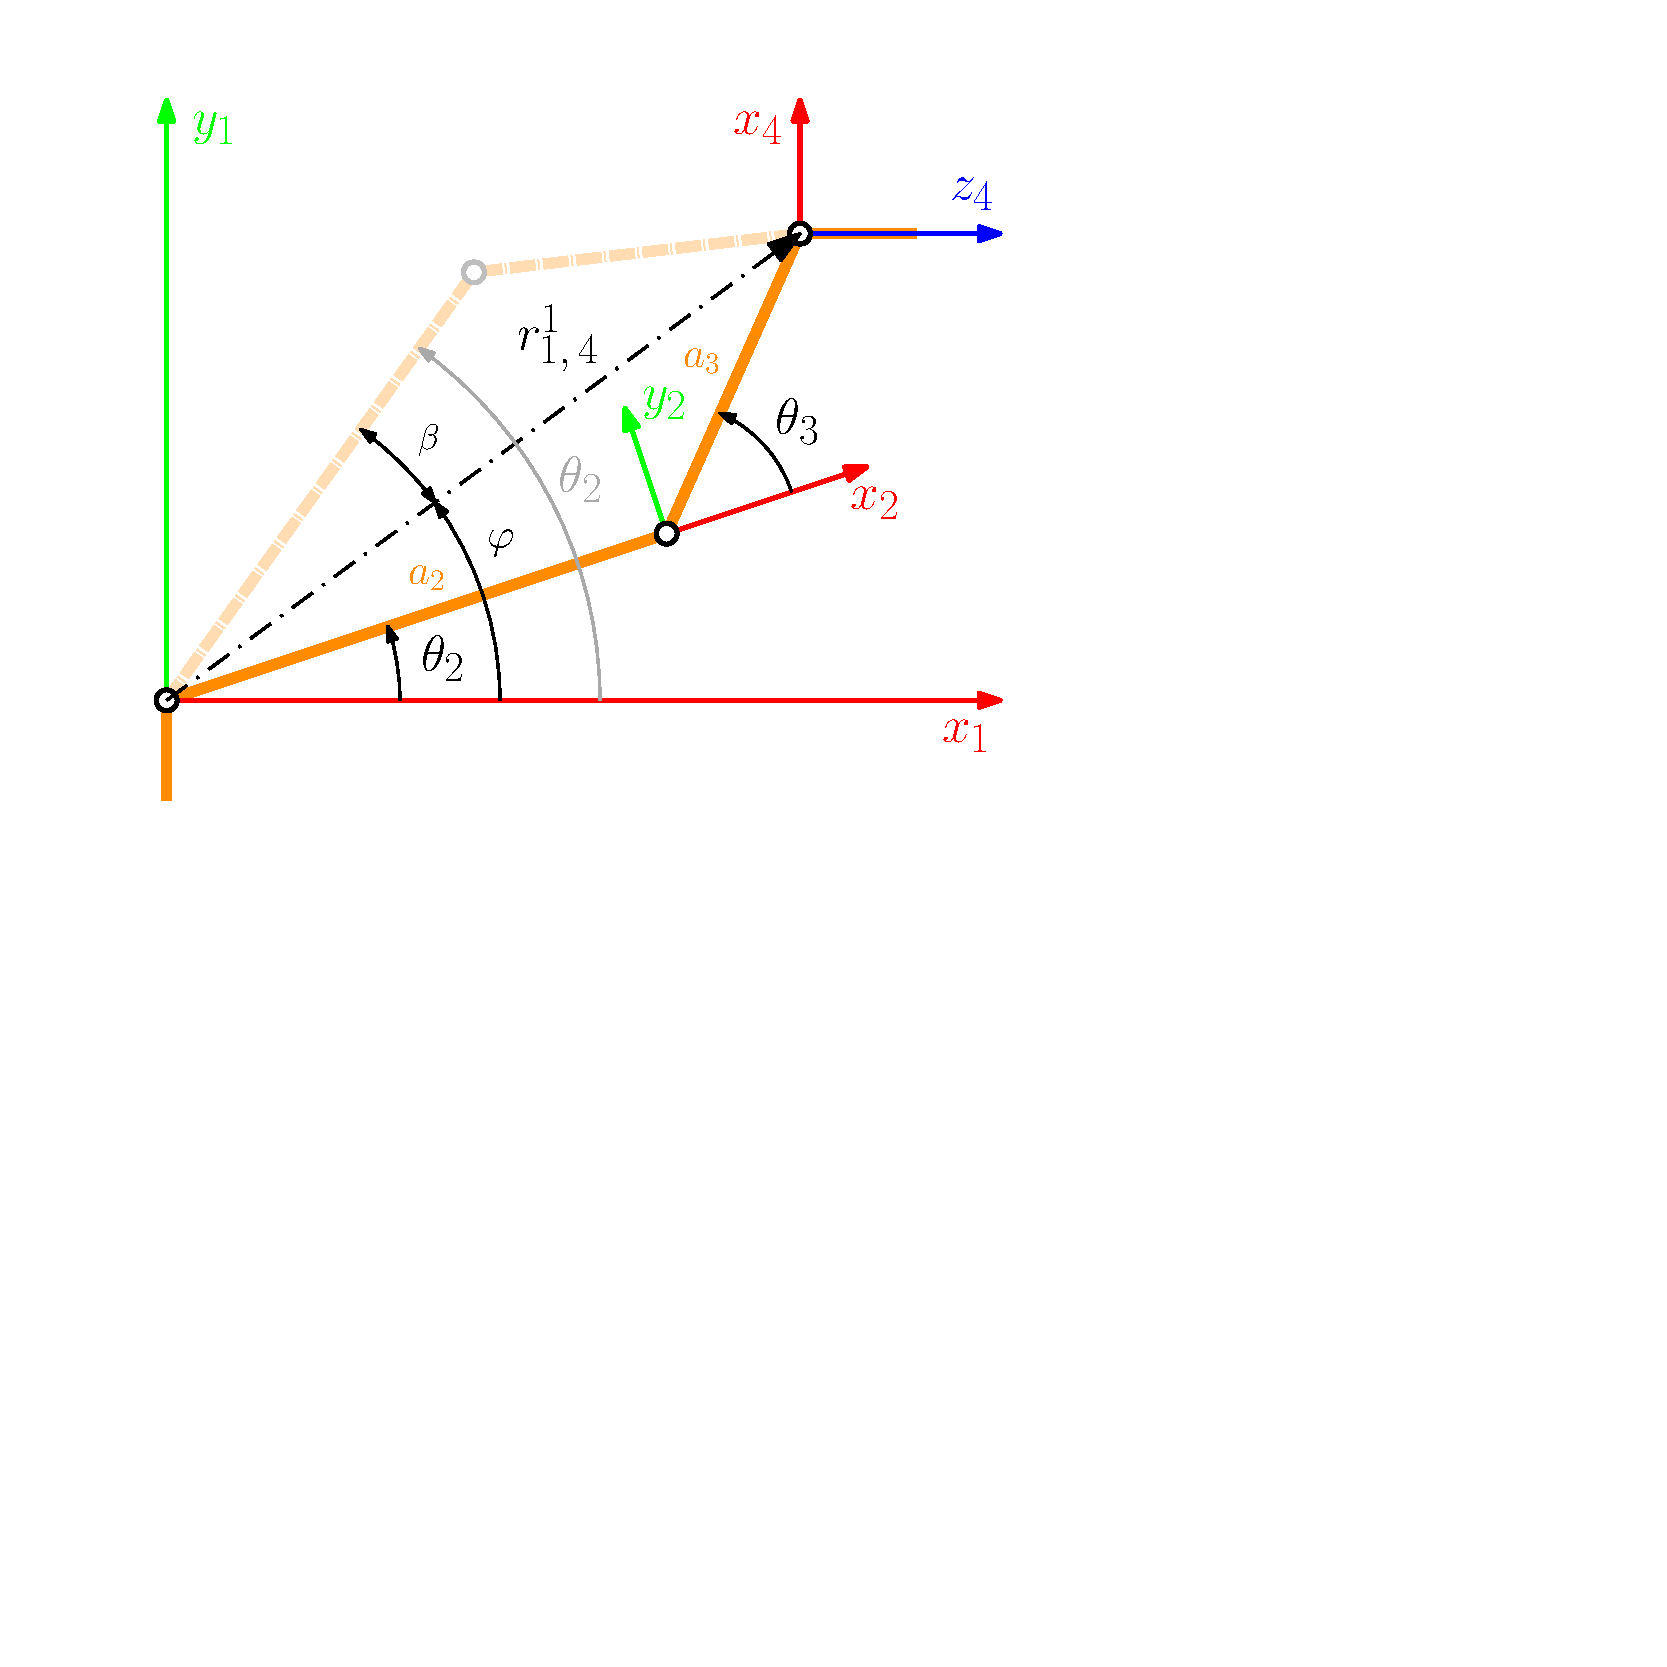
\includegraphics[width=0.58\textwidth]{ik_geometric_approach.pdf}
	\caption{Плоская часть манипулятора}
	\label{ik_geometric}
\end{figure}

По теореме косинусов, выражение для $\cos\theta_3$ (его зависимость от $\theta_1$ обуславливается зависимостью от этого угла вектора $r^1_{1,\,4}$) примет вид:
\begin{equation}
	c_3(\theta_1) = \frac{(r^1_{1,\,4})^T \!\! \cdot r^1_{1,\,4}- a_2^2 - a_3^2}{2 a_2 a_3}
\end{equation}
C~учетом этого для $\theta_3$ можно получить следующие выражения:
\begin{gather}
	\theta_3^\msf{I,II} = \mp \atan2\bigl(\sqrt{1 - c_3^2(\theta_1^\msf{I})},\; c_3(\theta_1^\msf{I})\bigr)\\
	\theta_3^\msf{III,IV} = \mp \atan2\bigl(\sqrt{1 - c_3^2(\theta_1^\msf{II})},\; c_3(\theta_1^\msf{II})\bigr)
\end{gather}

Как видно из рисунка~\ref{ik_geometric}, $\theta_2 = \varphi + \beta$ при $\theta_3^\msf{I,III} < 0$ и $\theta_2 = \varphi - \beta$ при $\theta_3^\msf{II,IV} > 0$.
Следовательно, принимая во внимание то, что
\begin{equation}
    \varphi(\theta_1) = \atan2(y_r,\, x_r),
    \qquad
    \beta(\theta_3) = \atan2(a_3\sin|\theta_3|,\: a_2 + a_3\cos|\theta_3|),
\end{equation}
где $x_r$ и $y_r$~--- проекции вектора $r^1_{1,\,4}$ на оси абсцисс и ординат (их значения см.~в~\eqref{eq_r_1_1_4}), для возможных значений угла $\theta_2$ можно записать:
\begin{align}
	\theta_2^\msf{I} &= \varphi(\theta_1^\msf{I}) + \beta(\theta_3^\msf{I}), &
	\theta_2^\msf{II} &= \varphi(\theta_1^\msf{I}) - \beta(\theta_3^\msf{II}),\\
	\theta_2^\msf{III} &= \varphi(\theta_1^\msf{II}) + \beta(\theta_3^\msf{III}), &
	\theta_2^\msf{IV} &= \varphi(\theta_1^\msf{II}) - \beta(\theta_3^\msf{IV})\ldotp
\end{align}

Выражения для значений угла $\theta_4$ после этого с учетом~\eqref{eq_theta_23_234} приобретают вид:
\begin{equation}
	\theta_4^\msf{I,II} = \theta_{234}^\msf{I} - \theta_{2}^\msf{I,II} - \theta_{3}^\msf{I,II},
	\qquad
	\theta_4^\msf{III,IV} = \theta_{234}^\msf{II} - \theta_{2}^\msf{III, IV} - \theta_{3}^\msf{III,IV}\ldotp
\end{equation}

Таким образом, любые положение и ориентацию схвата относительно основания манипулятор может обеспечить 4-мя собственными конфигурациями, которым соответствуют следующие наборы значений для его обобщенных координат $q=\left[q_1,\,q_2,\,q_3,\,q_4,\,q_5\right]^T$ (с~учетом таблицы~\ref{table_DH_params}):
\begin{align}
	\theta^\msf{I} &=
	\begin{bmatrix}
	    \theta_1^\msf{I} & \theta_2^\msf{I} & \theta_3^\msf{I} & \theta_4^\msf{I} & \theta_5^\msf{I}
	\end{bmatrix}^T\!\!\!\!\!,
	&
	\theta^\msf{II} &=
	\begin{bmatrix}
	    \theta_1^\msf{I} & \theta_2^\msf{II} & \theta_3^\msf{II} & \theta_4^\msf{II} & \theta_5^\msf{I}
	\end{bmatrix}^T\!\!\!\!\!,
	\\
	\theta^\msf{III} &=
	\begin{bmatrix}
	    \theta_1^\msf{II} & \theta_2^\msf{III} & \theta_3^\msf{III} & \theta_4^\msf{III} & \theta_5^\msf{II}
	\end{bmatrix}^T\!\!\!\!\!,
	&
	\theta^\msf{IV} &=
	\begin{bmatrix}
	    \theta_1^\msf{II} & \theta_2^\msf{IV} & \theta_3^\msf{IV} & \theta_4^\msf{IV} & \theta_5^\msf{II}
	\end{bmatrix}^T\!\!\!\!\!,
\end{align}
\begin{equation}
    q^\msf{I,II,III,IV} =
    \pi \cdot
    \begin{bmatrix}
	    \cfrac{169^\circ}{180^\circ} & \cfrac{65^\circ}{180^\circ} + \cfrac{1}{2} & -\cfrac{146^\circ}{180^\circ} &
	    \cfrac{102.5^\circ}{180^\circ} + \cfrac{1}{2} & \cfrac{167.5^\circ}{180^\circ}
	\end{bmatrix}^T
	\!\!- \; \theta^\msf{I,II,III,IV} \ldotp
\end{equation}

\vspace{0.5cm}
\subsubsection{Решение задач о скорости звеньев манипулятора}\label{part_kinematic_velocity}

%%\textbf{Приведем некоторые соотношения для скоростей и ускорений.}

Как видно из рассуждений в разделе~\ref{part_kinematic_position}, $i$-ое звено связано с СК, начало которой закрепленно в ($i+1$) сочленении. При этом кинематические параметры этого звена задаются в связанной с ним СК $Ox_{i-1}y_{i-1}z_{i-1}$.

Получим выражения, которые позволят последовательно получать скорости и ускорения звеньев манипулятора, начиная от базы в направлении схвата, выраженные в абсолютной СК $Ox_{0}y_{0}z_{0}$.

\begin{figure}[h!]
	\centering{\includegraphics[width=0.5\textwidth]{ipe/example_of_moving.pdf}}
	\caption{Рисунок, поясняющий приведённые в разделе~\ref{part_kinematic_velocity} выражения}
	\label{img:bodies}
\end{figure}

Заметим, что в соответствии с рисунком~\ref{img:bodies}, на котором изображена упрощенная кинематическая схема для двух соседних звеньев, радиус вектор
\begin{equation}\label{vector_r}
	r_{i-1, i} = r_i - r_{i-1}
\end{equation}
характеризует расположение СК $Ox_{i}y_{i}z_{i}$ относительно СК $Ox_{i-1}y_{i-1}z_{i-1}$.

Согласно~\eqref{vector_r} и теореме механики о сложении скоростей~\cite{yabl19964}, соотношения для  скоростей в подвижной и неподвижной системах координат запишутся:
\begin{equation}
	v_i = v_{i-1} + \omega_{i-1} \times r_{i-1,i} + \cfrac{d^* r_{i-1,i}}{dt},
\end{equation}
где $\frac{d^* r_{i-1,i}}{dt}$~--- скорость $i$-ого звена относительно СК $Ox_{i-1}y_{i-1}z_{i-1}$.

Для угловой скорости:
\begin{equation}\label{omega_i}
	\omega_i = \omega_{i-1} + \omega^{i-1}_{i},
	\quad
	\omega^{i-1}_{i} = z_{i-1} \cdot \dot{q}_i,
\end{equation}
где $\omega^{i-1}_{i}$~--- угловая скорость вращения СК $Ox_{i}y_{i}z_{i}$ относительно $Ox_{i-1}y_{i-1}z_{i-1}$, $\dot{q}_i$~--- угловая скорость вращения $i$-ого звена.

С учетом равенств~\eqref{vector_r}--\eqref{omega_i}, окончательно запишем рекуррентные соотношения для вычисления линейных и угловых скоростей манипулятора:
\begin{equation}\label{linear_velocities}
	v_i = v_{i-1} + \omega_{i} \times r_{i-1,i}, %%% + z_{i-1} \cdot \dot{q}_i,
\end{equation}

\begin{equation}\label{angular_velocities}
	\omega_i = \omega_{i-1} + z_{i-1} \cdot \dot{q}_i.
\end{equation}

Далее, согласно теореме о сложении ускорений, запишем соотношения для линейных и угловых ускорений:
\begin{equation}
	\dot{v}_i = \dot{v}_{i-1} + \omega_{i-1} \times (\omega_{i-1} \times r_{i-1,i}) + 2 \cdot \omega_{i-1} \times \cfrac{d^* r_{i-1,i}}{dt} + \cfrac{d^{*2} r_{i-1,i}}{dt^2},
\end{equation}
\begin{equation}
	\dot{\omega}_{i} = \dot{\omega}_{i-1} + \dot{\omega}^{i-1}_{i},
\end{equation}
где 
\begin{equation}
	\dot{\omega}^{i-1}_{i} = \cfrac{d^{*} \omega^{i-1}_{i}}{dt} + \omega_{i-1} \times \omega^{i-1}_{i},
	\quad
	\cfrac{d^{*} \omega^{i-1}_{i}}{dt} = z_{i-1} \cdot \ddot{q}_i.
\end{equation}

После элементарных преобразований, рекуррентные соотношения для линейных и угловых ускорений запишутся, как:
\begin{equation}\label{linear_accelerations}
	\dot{v}_i = \dot{v}_{i-1} + \omega_{i} \times (\omega_{i} \times r_{i-1,i}) + \dot{\omega}_i \times r_{i-1,i}, %%% + 2 \cdot \omega_{i} \times (z_{i-1} \cdot \dot{q}_i) + \dot{\omega}_{i} \times \dot{p}_{i-1,i} + z_{i-1} \cdot \ddot{q}_i,
\end{equation}
\begin{equation}\label{angular_accelerations}
	\dot{\omega}_i = \dot{\omega}_{i-1} + z_{i-1} \cdot \ddot{q}_i + \omega_{i-1} \times (z_{i-1} \cdot \dot{q}_i).
\end{equation}

Таким образом, соотношения~\eqref{linear_velocities}--\eqref{angular_velocities} и~\eqref{linear_accelerations}--\eqref{angular_accelerations} позволяют найти линейные и угловые скорости и ускорения звеньев, при $i=\overline{1,n}$ и начальных условиях $\omega = \dot{\omega} = v_0 = 0$, $\dot{v}_0 = g$, где $g$~--- вектор ускорения свободного падения.

Отсюда можно без труда получить конечные зависимости линейных и угловых скоростей. Для линейной скорости $k$-ого звена:
\begin{equation}
	v_k = \sum_{i = 1}^{k} z_{i-1} \times r_{i-1, k} \cdot \dot{q}_i.
\end{equation}
Для угловой скорости $k$-ого звена:
\begin{equation}
	\omega_k = \sum_{i = 1}^{k} z_{i-1} \cdot \dot{q}_i.
\end{equation}

Все векторы в рассмотренных соотношениях, описывающие движения манипулятора, заданы в базовой СК $Ox_{0}y_{0}z_{0}$. Руководствуясь соображениями вычислительной эффективности, представим векторы скоростей в СК их собственного звена. Тогда, если матрица перехода из СК $i$-ого звена $Ox_{i}y_{i}z_{i}$ в СК $Ox_{i-1}y_{i-1}z_{i-1}$, то:
\begin{equation}
	{}^{i-1}\!A_{i}^{-1} = 
	\begin{bmatrix}
		{}^{i-1}\!R_{i}^T	& {p}_{i-1,i} \\
		000	& 1
	\end{bmatrix}\!\!\!,
\end{equation}
где ${p}_{i-1,i} = {}^0\!R_{i-1}^T \cdot r_{i-1,i}$.

Можно переписать выражения ~\eqref{linear_velocities}--\eqref{angular_velocities} и~\eqref{linear_accelerations}--\eqref{angular_accelerations} в виде:
\begin{equation}
	v_i^i = {}^{i-1}\!R_{i} \cdot v^{i-1}_{i-1} + \omega^{i}_{i} \times p_{i-1,i},
\end{equation}
\begin{equation}
	\omega^{i}_{i} = {}^{i-1}\!R_{i} \cdot \omega^{i-1}_{i-1} + {}^{i-1}\!R_{i} \cdot z_0 \dot{q}_i,
\end{equation}
\begin{equation}
	\dot{v}^{i}_{i} = {}^{i-1}\!R_{i} \cdot \dot{v}^{i-1}_{i-1} + \omega^i_i \times (\omega^i_i \times p_{i-1,i}) + \dot{\omega}^i_i \times p_{i-1, i},
\end{equation}
\begin{equation}
	\dot{\omega}^i_i = {}^{i-1}\!R_{i} \cdot \dot{\omega}^i_i + {}^{i-1}\!R_{i} \cdot z_0 \ddot{q}_i + {}^{i-1}\!R_{i} \cdot \omega^{i-1}_{i-1} \times (z_0 \dot{q}_i).
\end{equation}

%%%
В задачах о скорости движения схвата манипулятора описывается вектором $\mathbf{s} = [x,y,z,\varphi, \psi, \theta]$, линейной $ \bm{v} $ и угловой $ \bm{\omega} $ скоростями, где со схватом связана СК $ Ox_{n}y_{n}z_{n} $. Вектор $ \mathbf{s} $ определяется конфигурацией манипулятора, задаваемой вектором обобщеннных координат $ \mathbf{q} = [q_1, q_2, \dots, q_n]^T $, что можно записать, как:
\begin{equation}\label{s_fq}
	\mathbf{s} = f (\mathbf{q}).
\end{equation}

Дифференцируя~\eqref{s_fq} по времени, получаем:
\begin{equation}\label{sjq}
	\dot{\mathbf{s}} = J (\mathbf{q}) \cdot \dot{\mathbf{q}},
\end{equation}
где $ \dot{\mathbf{s}} $ вектор скорости схвата:
\begin{equation}\label{fvk_1}
	\dot{\mathbf{s}} =
	\begin{bmatrix}
			\bm{v} \\ 
		\bm{\omega}
	\end{bmatrix}\!\!\!,
\end{equation}
$ J(\mathbf{q}) $~--- матрица Якоби размерности $ 6 \times n $, $\dot{\mathbf{q}} = [\dot{q}_1, \dot{q}_2, \dots, \dot{q}_n]^T $~--- вектор скоростей обобщенных координат.

%\subsubsection{Прямая задача о скорости}
\textbf{Прямая задача о скорости} формулируется, как нахождение линейной~$ \bm{v} $ и угловой~$ \bm{\omega} $ скоростей схвата по известным скоростям обобщенных координат $ \dot{q}_1, \dot{q}_2, \dots, \dot{q}_n $.
Заметим, что из~\eqref{linear_velocities}--\eqref{angular_velocities} следует, что если записать матрицу Якоби в виде:
\begin{equation}\label{Jq}
	J(\mathbf{q}) = 
	\begin{bmatrix}
	\bm{j}_1 & \bm{j}_2 & \cdots & \bm{j}_n
	\end{bmatrix},
\end{equation}
то вектор $ \bm{j}_k $ будет рассчитываться из выражения:
\begin{equation}
	\bm{j}_k = 
	\begin{bmatrix}
	z_{k-1} \\
	z_{z-1} \times p_{k-1,n}
	\end{bmatrix},
\end{equation}

Следовательно, выражение~\eqref{sjq} является решением прямой задачи о скорости, где матрица $ J(\mathbf{q}) $ находится из~\eqref{Jq}.

Матрицу Якоби получим, используя дифференциальные преобразования. Обозначим матрицу Якоби, как:
\begin{equation}\label{J}
	J = 
	\begin{bmatrix}
		J_v \\ 
		J_{\omega}
	\end{bmatrix}\!\!\!,
\end{equation}
тогда перепишем соотношения для скоростей в виде
\begin{align}
	\label{Jv1}
	\bm{v}  = J_{v} \dot{\bm{q}}, \\
	\label{Jw1}
	\bm{\omega} = J_{\omega} \dot{\bm{q}}.
\end{align}

\begin{figure}[h!]
	\begin{minipage}[h]{0.5\linewidth}
		\centering{\includegraphics[width=0.95\linewidth]{ipe/diff_matrix_v2.pdf} \\ а)}
	\end{minipage}
	\hfill
	\begin{minipage}[h]{0.5\linewidth}
		\centering{\includegraphics[width=0.95\linewidth]{ipe/diff_transform_v2.pdf} \\ б)}
	\end{minipage}
	\caption{а~--- дифференциальное перемещение, б~--- изменение матрицы трансфорации при дифференциальном перемещении}
	\label{img:diff_transformations}
\end{figure}

Если представить малое изменение матрицы трансформации $ T $ (рисунок~\ref{img:diff_transformations}a), как
\begin{equation}
	\tilde{T} = T + dT,
\end{equation}
откуда $ dT = \tilde{T} - T = \tilde{T}(d\bm{r}, \delta\bm{\varphi}) - T$, где $ d\bm{r} $ и $ \delta\bm{\varphi} $~--- малые перемещение и поворот соответственно, то для k-ого звена манипулятора,  применяя правило дифференцирования матриц однородных преобразований $ \cfrac{\partial A_k}{\partial q_l} = \theta_k \cdot A_k $, можно получить:
\begin{equation}\label{dkT}
	d_k T = A_1 A_2 \dots A_{k-1} \theta_k dq_k A_{k+1} \dots A_{n-1} A_n,
\end{equation}
где 
\begin{equation}
	\theta_k = 
	\begin{bmatrix}
	0 & -1 & 0 & 0 \\
	1 & 0 & 0 & 0 \\
	0 & 0 & 0 & 0 \\
	0 & 0 & 0 & 0
	\end{bmatrix}
\end{equation}

Выражение~\eqref{dkT} можно переписать в виде:
\begin{equation}
	d_k T = \Delta_{\theta_k} \cdot T,
\end{equation}
где $ \Delta_{\theta_k} $~--- матрица дифференциальных преобразований:
\begin{equation}\label{Delta_matrix}
	\Delta_{\theta_k} = T_{k-1} \theta_k T_{k-1}^{-1} dq_k.
\end{equation}

Обозначим разыскиваемые дифференциальные перемещения  схвата манипулятора, как~$ d \bm{r}_n $ и~$\delta\bm{\varphi}_n $, изображённые на рисунке~\ref{img:diff_transformations}б, тогда матрица дифференциальных преобразований:
\begin{equation}
	\Delta_n =
	\begin{bmatrix}
		0 & - \delta z_n & \delta y_n & d x_n \\
		\delta z_n & 0 & -\delta x_n & d y_n \\
		-\delta y_n & \delta x_n & 0 & d z_n \\
		0 & 0 & 0 & 0
	\end{bmatrix}
	=
	\left[
	\begin{array}{c:c}
	\Omega_{\delta\bm{\varphi}_n} & d \bm{r}_n \\ \hdashline
	000 &  0
	\end{array}
	\right]\!\!\!.
\end{equation}

Раскрыв~\eqref{Delta_matrix}, получим:
\begin{equation}
	\left[
	\begin{array}{c:c}
		\Omega_{\delta\bm{\varphi}_n} & d\bm{r}_n - \Omega_{\delta\bm{\varphi}_n} \cdot {p}_n \\ \hdashline
		000 &  0
	\end{array}
	\right]
	=
	\left[
	\begin{array}{c:c}
		R_{k-1} \Omega_{001} R_{k-1}^T & - R_{k-1} \Omega_{001} R_{k-1}^T {p}_{k-1} \\ \hdashline
		000 &  0
	\end{array}
	\right]
	dq_k,
\end{equation}
где 
\begin{gather}
	\label{dr}
	d\bm{r}_n = \Omega_{\delta\bm{\varphi}_n} \cdot {p}_n - R_{k-1} \cdot \Omega_{001} \cdot R_{k-1}^T \cdot {p}_{k-1} \cdot dq_k, \\
	\label{Omega_phi}
	\Omega_{\delta\bm{\varphi}_n} = R_{k-1} \cdot \Omega_{001} \cdot R_{k-1}^T \cdot dq_k,
\end{gather}
$ \Omega_{001} $~--- матрица, задающая вращение вокруг вектора $ [0,0,1]^T $.

Вращение вокруг оси $ z_{k-1} $ определяется выражением:
\begin{equation}
	z_{k-1} = R_{k-1} \cdot
	\begin{bmatrix}
	0 \\ 0 \\ 1
	\end{bmatrix}\!\!\!,
\end{equation}
тогда, в силу~\eqref{Omega_phi} и \eqref{dr}, имеем
\begin{gather}
	\label{diff_dr}
	d\bm{r}_n = z_{k-1} \times (p_n - p_{k-1}) \cdot dq_k, \\
	\label{diff_delta_phi}
	\delta\bm{\varphi}_n = z_{k-1} \cdot dq_k.
\end{gather}

Из выражения~\eqref{diff_delta_phi} видим, что расчет матрицы Якоби $ J_\omega $ из выражения~\eqref{J} не представляет труда, так как векторы $ z_i $ легко извлекаются из матриц трансформации $ T_i $ (третий столбец).

%\textcolor{red}{Представим альтернативную форму представления матрицы Якоби, позволяющую эффективнее производить ее вычисления...}

Из выражений~\eqref{diff_delta_phi}--\eqref{diff_dr} и~\eqref{J} получим все матрицы Якоби для рассматриваемого манипулятора:

\begin{gather*}
	J_{\omega 1} =
	\begin{bmatrix}
		z^0_0 & \nv & \nv & \nv & \nv
	\end{bmatrix}\!\!,
	\qquad
	J_{\omega 2} =
	\begin{bmatrix}
		z^0_0 & z^0_1 & \nv & \nv & \nv
	\end{bmatrix}\!\!,
	\\
	J_{\omega 3} =
	\begin{bmatrix}
		z^0_0 & z^0_1 & z^0_2 & \nv & \nv
	\end{bmatrix}\!\!,
	\qquad
	J_{\omega 4} =
	\begin{bmatrix}
		z^0_0 & z^0_1 & z^0_2 & z^0_3 & \nv
	\end{bmatrix}\!\!,
	\\
	J_{\omega 5} =
	\begin{bmatrix}
		z^0_0 & z^0_1 & z^0_2 & z^0_3 & z^0_4
	\end{bmatrix}\!\!,
\end{gather*}
где $\nv = [0\;0\;0]^T$~--- нулевой вектор.

\begin{gather*}
J_{v1} =
\begin{bmatrix}
z^0_0 \times \left( r^0_{0,\,1} - r^0_{0,\,0}\right) & \nv & \nv & \nv & \nv
\end{bmatrix}\!\!,
\\
J_{v2} =
\begin{bmatrix}
z^0_0 \times \left( r^0_{0,\,2} - r^0_{0,\,0}\right) & z^0_1 \times \left( r^0_{0,\,2} - r^0_{0,\,1}\right) & \nv & \nv & \nv
\end{bmatrix}\!\!,
\\
J_{v3} =
\begin{bmatrix}
z^0_0 \times \left( r^0_{0,\,3} - r^0_{0,\,0}\right) & z^0_1 \times \left( r^0_{0,\,3} - r^0_{0,\,1}\right) &
z^0_2 \times \left( r^0_{0,\,3} - r^0_{0,\,2}\right) & \nv & \nv
\end{bmatrix}\!\!,
\end{gather*}
\begin{gather*}
J_{v4} =
\begin{bmatrix}
z^0_0 \times \left( r^0_{0,\,4} - r^0_{0,\,0}\right) \\
z^0_1 \times \left( r^0_{0,\,4} - r^0_{0,\,1}\right) \\
z^0_2 \times \left( r^0_{0,\,4} - r^0_{0,\,2}\right) \\
z^0_3 \times \left( r^0_{0,\,4} - r^0_{0,\,3}\right) \\
\nv
\end{bmatrix}^T\!\!\!\!\!,
\qquad
J_{v5} =
\begin{bmatrix}
z^0_0 \times \left( r^0_{0,\,5} - r^0_{0,\,0}\right) \\
z^0_1 \times \left( r^0_{0,\,5} - r^0_{0,\,1}\right) \\
z^0_2 \times \left( r^0_{0,\,5} - r^0_{0,\,2}\right) \\
z^0_3 \times \left( r^0_{0,\,5} - r^0_{0,\,3}\right) \\
z^0_4 \times \left( r^0_{0,\,5} - r^0_{0,\,4}\right)
\end{bmatrix}^T\!\!\!\!\!.
\end{gather*}


%\subsubsection{Обратная задача о скорости}
\textbf{Обратная задача о скорости} формулируется как поиск неизвестных скоростей обобщенных координат при известных линейной и уголовой скоростях схвата. Соотношения записывается как система шести линейных уравнений с $ n $ неизвестными $ \dot{q}_1, \dot{q}_2, \dots, \dot{q}_n $:
\begin{equation}\label{ivp}
	\dot{\mathbf{q}} =  J^{-1}(\mathbf{q})\dot{\mathbf{s}}.
\end{equation}

Решение~\eqref{ivp} существует тогда и только тогда, когда 
\begin{equation}
	rank(J(\mathbf{q})) = rank([J(\mathbf{q}), \dot{\mathbf{s}}]).
\end{equation}

Для пятистепенного манипулятора KUKA Youbot возможны три случая:
\begin{enumerate}
	\item $rank(J) \ne rank([J, \dot{\mathbf{s}}])$~--- не имеет решений;
	\item $rank(J) = rank([J, \dot{\mathbf{s}}])$~--- имеет единственное решение;
	\item $rank(J) = rank([J, \dot{\mathbf{s}}])$~--- бесконечное множество решений.
\end{enumerate}

Таким образом, в сингулярных конфигурациях манипулятора матрица Якоби не позволяется установить однозначную зависимость в~\eqref{ivp}. Поиск решений уравнения~\eqref{ivp} является частью алгоритма управления манипулятором.





\subsection{Система кинематического управления}\label{part_kinematic_control}

Кинематическое управление реализуется в два этапа: первый включает в себя получение траектории движения сочленений манипулятора $ \bm{q}(t) $ или схвата $ \bm{s}(t) $ на интервале времени $ t \in [t_s,\,\,t_f] $; второй этап подразумевает синтез системы управления, способной отработать спланированную траекторию.

Планированию траекторий посвящён следующий раздел. Здесь реализуем систему управления для следования по заданной траектории.

\begin{figure}[h!]
	\centering{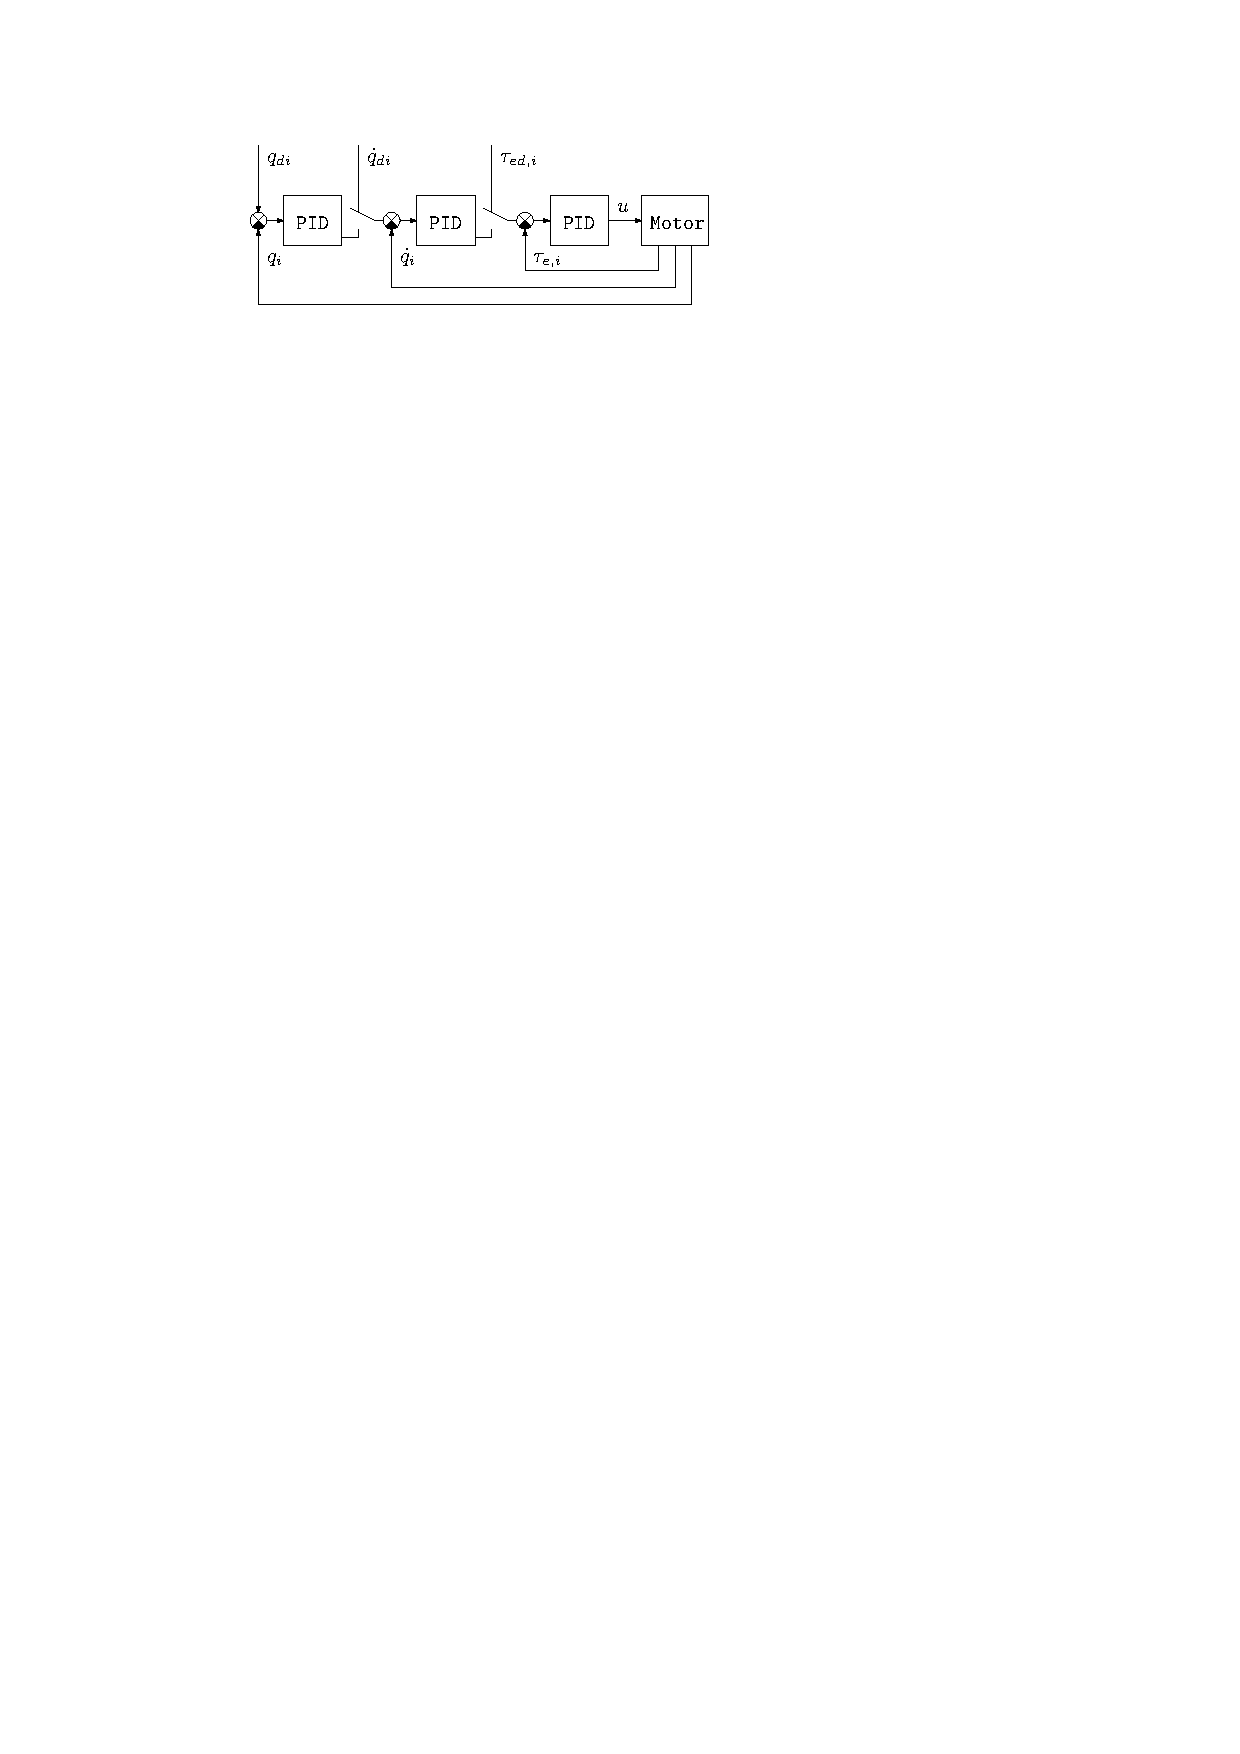
\includegraphics[width=0.7\textwidth]{structure_of_actuator_cs.pdf}}
	\vspace{0.5cm}
	\caption{Структурная схема системы управления приводами, встроенная в контроллеры манипулятора}
	\label{img:structure_of_actuator_cs}
\end{figure}

Каждый из приводов манипулятора робота KUKA Youbot имеет собственную систему управления, структура которой иллюстрируется схемой, представленной на рисунке~\ref{img:structure_of_actuator_cs}. Из нее видно, что каждый из приводов робота может управляться заданием значения для угла $ q_{di} $, или скорости $ \dot{q}_{di} $, или момента силы $ \tau_{ed,i} $, который должен быть на нем обеспечен. Это значение подается на вход соответствующего ПИД-регулятора, коэффициенты которого доступны настройке, и далее (уже в виде сигнала напряжения u) на контролируемый двигатель.

Далее в тексте будет рассмотрена система управления, в которой в качестве управляющего сигнала рассматриваются векторы $ \bm{q} $ и $ \dot{\bm{q}} $. Из величин, описывающих состояние робота в данный момент времени, в используемом ПО доступны векторы $\bm{q}(t)$, $\dot{\bm{q}}(t)$ и $\bm\tau_e (t)$.

Цель управления в минимизации ошибки между заданной траекторией и положением схвата в каждый момент времени. Введём обозначения: траекторию обозначим, как:
\begin{equation}
	\bm{s}_d = 
	\begin{bmatrix}
		\bm p_d \\
		\bm\varphi_d
	\end{bmatrix}
	= f(\bm{q}_d),
	\quad
	\dot{\bm{s}}_d = 
	\begin{bmatrix}
		v_d \\
		\omega_d
	\end{bmatrix}
	 = f(\dot{\bm{q}}_d),
\end{equation}
а текущее положение схвата:
\begin{equation}
	\bm{s} = 
	\begin{bmatrix}
		\bm p \\
		\bm\varphi
	\end{bmatrix}
	= f(\bm{q}),
	\quad
	\dot{\bm{s}} = 
	\begin{bmatrix}
		v \\
		\omega
	\end{bmatrix}
	= f(\dot{\bm{q}}),
\end{equation}

%%%\textcolor{red}{Расчёт текущего положения схвата осуществляется методом Ньютона, который касательные и все такое, описанного в~\ref{part_newton}. ДОБАВИТЬ ЧАСТЬ В РЕШЕНИЕ ЗАДАЧ КИНЕМАТИКИ!!1}

%%%%%%%%%%%%%%%
%\textbf{Управление по вектору скорости.}

Для следования по траектории, заданной функциями $ \bm{s}_d(t) $ и  $ \dot{\bm{s}}_d(t) $ реализуем управление по вектору скорости, которое формулируется как минимизация ошибки скорости следования по траектории. Воспользуемся соотношением для обратной задачи о скорости:
\begin{equation}
	\dot{\bm{q}} = J^+(q) \dot{\bm{s}},
\end{equation}
где $ \bm{q} $~--- вектор обобщенных координат, $ \bm{s} $~--- вектор, определяющий положение схвата, $ J^+ $~--- псевдообратная матрица (так как размерность матрицы Якоби для рассматриваемого манипулятора $[6\times 5]$).

Введем ошибку по положению схвата:
\begin{equation}\label{error}
	\bm{e}(t) = \bm{s}_d(t) - \bm{s}(t).
\end{equation}
Затем, дифференцируя~\eqref{error} по времени, получим:
\begin{equation}
	\dot{\bm{e}}(t) = \dot{\bm{s}}_d(t) - \dot{\bm{s}}(t) =
	\dot{\bm{s}}_d(t) - J^+(q) \dot{\bm{q}}.
\end{equation}
Необходимо выбрать вектор $ \dot{\bm{q}}(t) $ таким, чтобы выполнялось условие
\begin{equation}
	\lim_{t\to\infty} \dot{\bm{e}}(t) = 0.
\end{equation}
Тогда, если
\begin{equation}
	\dot{\bm{q}}(t) = J^+(q) \cdot (\dot{\bm{s}}_d(t) - \dot{\bm{e}}(t)),
\end{equation}
то, выбрав 
\begin{equation}
	\dot{\bm{e}}(t) = - K {\bm{e}}(t),
\end{equation}
можно обеспечить асимптотическую устойчивость системы управления.

Схема системы управления изображена на рисунке~\ref{img:velocity_control_system}.
\begin{figure}[h!]
	\centering{\includegraphics[width=1\textwidth]{ipe/velocity_control_system.pdf}}
	\caption{Система управления по вектору скорости}
	\label{img:velocity_control_system}
\end{figure}

В следующем разделе рассмотрим способы задания траектории, которую в последствии будем подавать на вход синтезированной системы управления.



%\subsection{Динамическая модель манипулятора}\label{part_dynamic_model}
\subsubsection{Динамические уравнения}

Для описание динамики манипулятора вводятся в рассмотрение барицентрические СК $Ox_{ci}y_{ci}z_{ci}$\lefteqn,\footnote{Системы координат, чьи начала совпадают с центрами масс соответствующих звеньев.} где $i=\overline{1,5}$, показанные на рисунке~\ref{img_mass_frames}.
Причем, каждая СК $Ox_{ci}y_{ci}z_{ci}$ сонаправлена с~$Ox_iy_iz_i$.

\begin{figure}[h!]
	\centering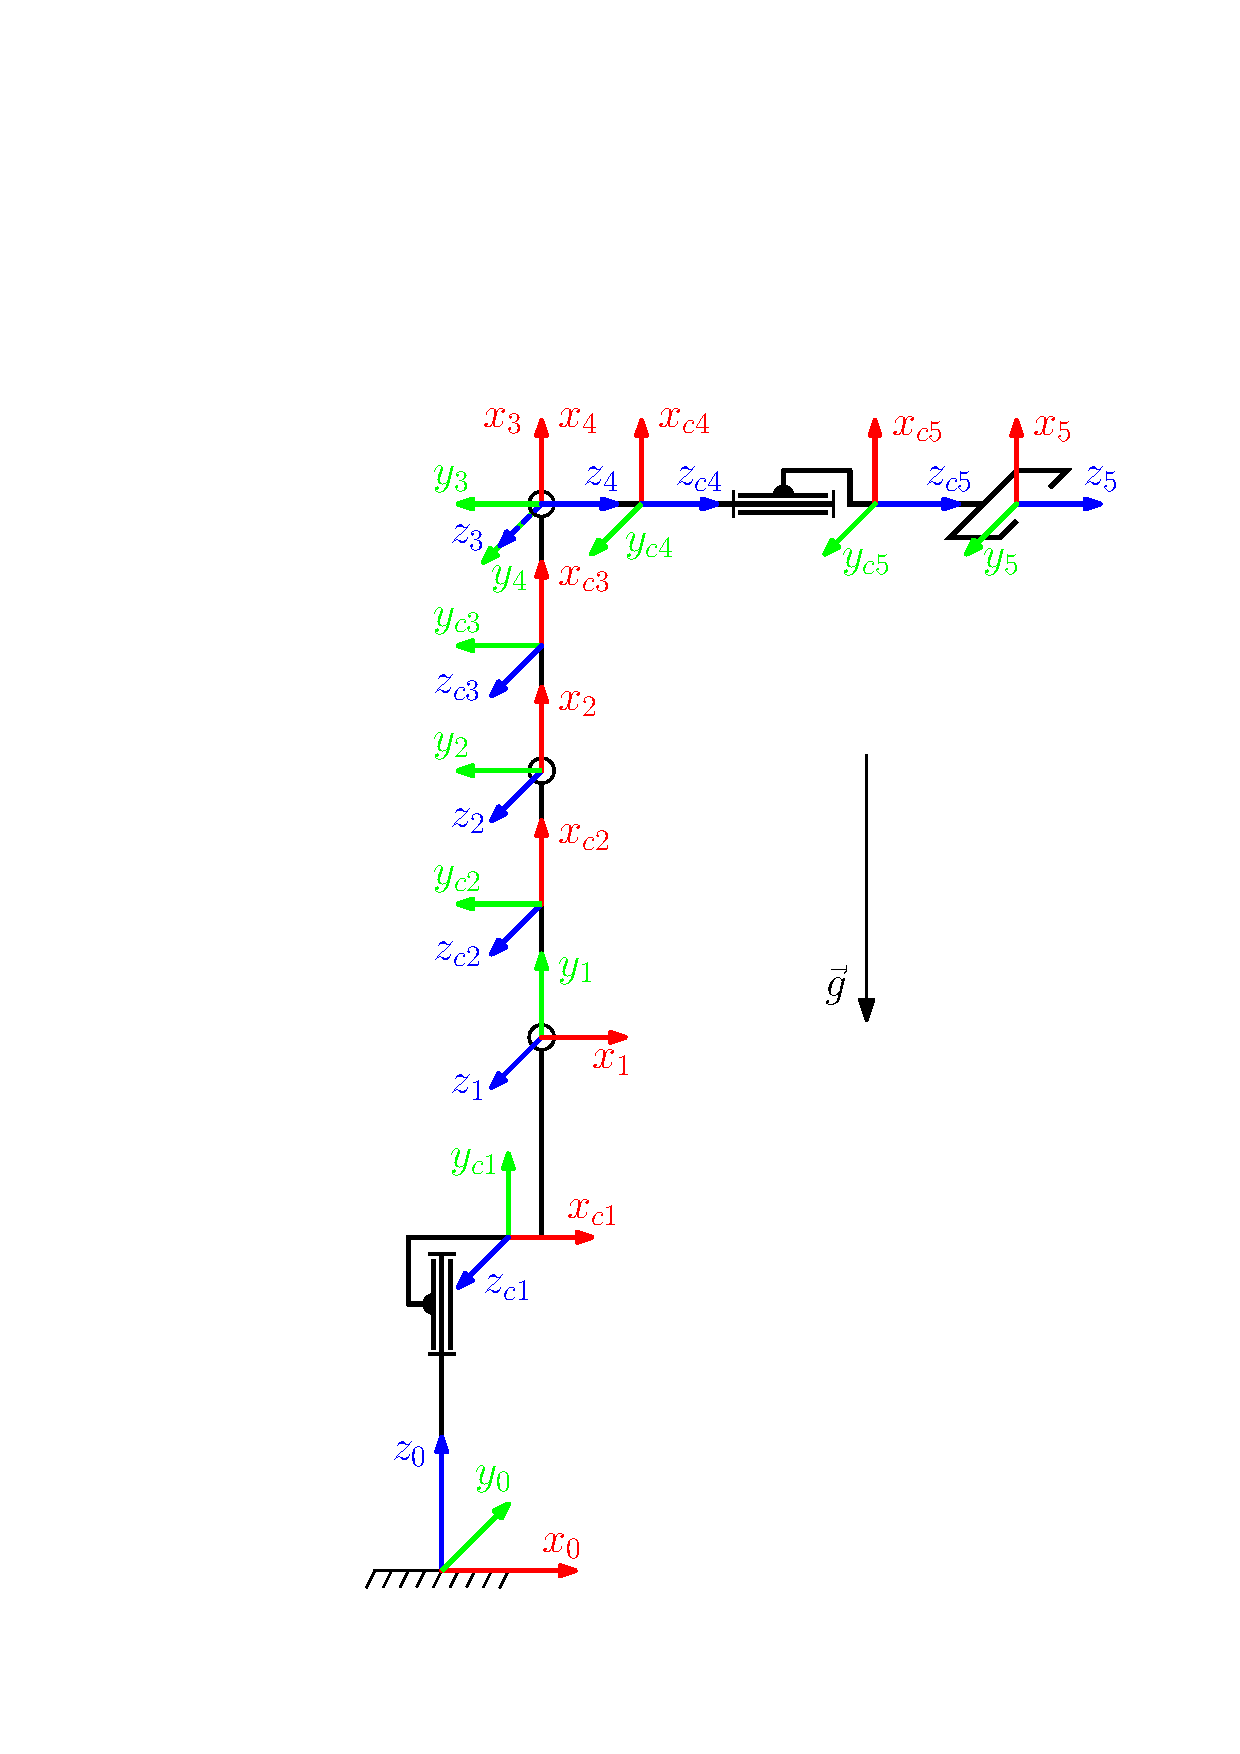
\includegraphics[height=16.5cm]{kinematics_mass_frames.pdf}
	\caption{Положение барицентрических СК и направление вектора $\vec{g}$.}
	\label{img_mass_frames}
\end{figure}

Для описания положения введенных СК используются следующие векторы:
\begin{equation}
    r^i_{i,\,ci} =
    \begin{bmatrix}
        x_{ci} \\ y_{ci} \\ z_{ci}
    \end{bmatrix}\!\!,\quad i = \overline{1,5},
\end{equation}
где $x_{ci}$, $y_{ci}$ и $z_{ci}$~--- некоторые постоянные величины, $r^i_{j,k}$~--- вектор из начала $Ox_{j}y_{j}z_{j}$ в начало $Ox_{k}y_{k}z_{k}$, выраженный относительно $Ox_{i}y_{i}z_{i}$.

Для компонент тензоров инерции $\mathcal{I}^{i}_i = const$ вводятся обозначения:
\begin{equation}
    \mathcal{I}^{i}_i =
    \begin{bmatrix}
        I_{i,\,xx} & I_{i,\,xy} & I_{i,\,xz} \\
        I_{i,\,xy} & I_{i,\,yy} & I_{i,\,yz} \\
        I_{i,\,xz} & I_{i,\,yz} & I_{i,\,zz}
    \end{bmatrix}\!\!\ldotp
\end{equation}

Вектор гравитации имеет вид:
\begin{equation}
    g_0 =
    \begin{bmatrix}
        0 \\ 0 \\ -g
    \end{bmatrix}\!\!,
\end{equation}
где $g=9.82\text{ м}/\text{с}^2$.

Ниже приводятся формулы для расчета величин, которые потребуются в дальнейшем (далее везде $i = \overline{1,5}$):
\begin{itemize}
    \item для расчета $r^0_{0,\,i}$ и ${}^{0}R_i$:
        \begin{equation}
            {}^0A_i = {}^0A_1 \cdot {}^1A_2 \cdot \ldots \cdot {}^{i-1}A_i;
        \end{equation}
    \item для расчета $r^i_{0,\,i}$:
        \begin{gather}
            r^i_{0,\,i} = {}^{0}R_i^T \cdot r^0_{0,\,i};
        \end{gather}
    \item для расчета $z^0_i$:
        \begin{equation}
            z^0_i = {}^{0}R_i \cdot z^i_i = {}^{0}R_i \cdot
            \begin{bmatrix}
                0 \\ 0 \\ 1
            \end{bmatrix}\!\!;
        \end{equation}
    \item для расчета $g_i$, $v^i_i$ и $\omega^i_i$:
        \begin{equation}\label{eq_transform_of_g_v_omega}
            g_i = {}^{0}R_i^T \cdot g_0,
            \qquad
            v^i_i = {}^{0}R_i^T \cdot v^0_i,
            \qquad
            \omega^i_i = {}^{0}R_i^T \cdot \omega^0_i \ldotp
        \end{equation}
\end{itemize}

%%%%%%%%%%%%%%%%%%%%%%%%%%%%%%%%%%%%%%%%%%%%%%%
%%%%%%%%%%%%%%%%%%%%%%%%%%%%%%%%%%%%%%%%%%%%%%%
%%%%%%%%%%%%%%%%%%%%%%%%%%%%%%%%%%%%%%%%%%%%%%%
\textbf{Вывод уравнений движения}

Для синтеза системы управления, модель манипулятора нужно представить в матричном виде:
\begin{equation}\label{simple_dynamics}
	\tau = D(q) \ddot{q} + C(q,\dot{q}) \dot{q} + G(q),
\end{equation}
где $D(q)$~--- матрица инерции, $C(q,\dot{q})$~--- матрица центробежных и Кориолисовых сил, $G(q)$~--- вектор гравитации, $\tau$~--- вектор моментов.

Выражение для матрицы~$D(q)$ может быть найдено из формулы для кинетической энергии с учетом того, что справедливо
\begin{equation}\label{eq_K_in_form_with_D}
	\left\{
	\begin{aligned}
	\!& K = \frac{1}{2} \, \dot{q}^T D(q) \dot{q}, \\
	\!& D(q) = D^T\!(q),
	\end{aligned}
	\right.
\end{equation}
для матрицы $C(q,\dot{q})$~--- из выражения для $D(q)$ в соответствии с формулами:
\begin{gather}
	C_{ijk} = \cfrac{1}{2} \left( \cfrac{\partial D_{kj}}{\partial q_i} + \cfrac{\partial D_{ki}}{\partial q_j} - \cfrac{\partial D_{ij}}{\partial q_k}\right)\!\!,
	\\
	C_{kj} = \sum_{i = 1}^n C_{ijk} \dot{q}_i,
\end{gather}
где $D_{ij}$, $C_{ij}$~--- элементы матриц $D(q)$ и $C(q,\dot{q})$ соответственно, стоящие на пересечении $i$-ой строки и $j$-го столбца;
а для вектора $G(q)$~--- по формуле
\begin{equation}
	G(q) =
	\begin{bmatrix}
		\cfrac{\partial U}{\partial q_1} &
		\cfrac{\partial U}{\partial q_2} &
		\dots &
		\cfrac{\partial U}{\partial q_5}
	\end{bmatrix}^T\!\!\!\!\!\ldotp
\end{equation}

Потенциальная энергия манипулятора
\begin{equation}
    U =  -\sum_{i=1}^5 \left( m_i g_i^T r^i_{0,\,ci} \right) = -\sum_{i=1}^5 \left( m_i g_i^T r^i_{0,\,i} + g_i^T (m_ir^i_{i,\,ci}) \right)\!.
\end{equation}

Кинетическая энергия манипулятора
\begin{equation}\label{eq_eq_for_K_for_linear_model}
	K = \sum_{i=1}^5 \left( \frac{1}{2} m_i (v^i_i)^T v^i_i + \frac{1}{2} (\omega^i_i)^T \mathcal{I}^{i}_i \omega^i_i + (m_ir^i_{i,\,ci})^T \cdot (v^i_i \times \omega^i_i) \right)  \ldotp
\end{equation}

Якобианы, устанавливающие в соответствии с формулой
\begin{equation}\label{eq_work_of_lin_jacobians}
    v^0_{i} = -J_{vi}\dot{q}, \quad i = \overline{1,5}
\end{equation}
связь между линейными скоростями начал соответствующих СК и вектором~$\dot{q}$:
\begin{gather}
    J_{v1} =
    \begin{bmatrix}
        z^0_0 \times \left( r^0_{0,\,1} - r^0_{0,\,0}\right) & \nv & \nv & \nv & \nv
    \end{bmatrix}\!\!,
    \\
    J_{v2} =
    \begin{bmatrix}
        z^0_0 \times \left( r^0_{0,\,2} - r^0_{0,\,0}\right) & z^0_1 \times \left( r^0_{0,\,2} - r^0_{0,\,1}\right) & \nv & \nv & \nv
    \end{bmatrix}\!\!,
    \\
    J_{v3} =
    \begin{bmatrix}
        z^0_0 \times \left( r^0_{0,\,3} - r^0_{0,\,0}\right) & z^0_1 \times \left( r^0_{0,\,3} - r^0_{0,\,1}\right) &
        z^0_2 \times \left( r^0_{0,\,3} - r^0_{0,\,2}\right) & \nv & \nv
    \end{bmatrix}\!\!,
    \\
    J_{v4} =
    \begin{bmatrix}
        z^0_0 \times \left( r^0_{0,\,4} - r^0_{0,\,0}\right) \\
        z^0_1 \times \left( r^0_{0,\,4} - r^0_{0,\,1}\right) \\
        z^0_2 \times \left( r^0_{0,\,4} - r^0_{0,\,2}\right) \\
        z^0_3 \times \left( r^0_{0,\,4} - r^0_{0,\,3}\right) \\
        \nv
    \end{bmatrix}^T\!\!\!\!\!,
    \qquad
    J_{v5} =
    \begin{bmatrix}
        z^0_0 \times \left( r^0_{0,\,5} - r^0_{0,\,0}\right) \\
        z^0_1 \times \left( r^0_{0,\,5} - r^0_{0,\,1}\right) \\
        z^0_2 \times \left( r^0_{0,\,5} - r^0_{0,\,2}\right) \\
        z^0_3 \times \left( r^0_{0,\,5} - r^0_{0,\,3}\right) \\
        z^0_4 \times \left( r^0_{0,\,5} - r^0_{0,\,4}\right)
    \end{bmatrix}^T\!\!\!\!\!,
\end{gather}
где $\nv = [0\;0\;0]^T$~--- нулевой вектор.

Якобианы, устанавливающие в соответствии с формулой
\begin{equation}\label{eq_work_of_ang_jacobians}
    \omega^0_{i} = -J_{\omega i}\dot{q}, \quad i = \overline{1,5}
\end{equation}
связь между угловыми скоростями звеньев и вектором~$\dot{q}$:
\begin{gather}
    J_{\omega 1} =
    \begin{bmatrix}
        z^0_0 & \nv & \nv & \nv & \nv
    \end{bmatrix}\!\!,
    \qquad
    J_{\omega 2} =
    \begin{bmatrix}
        z^0_0 & z^0_1 & \nv & \nv & \nv
    \end{bmatrix}\!\!,
    \\
    J_{\omega 3} =
    \begin{bmatrix}
         z^0_0 & z^0_1 & z^0_2 & \nv & \nv
    \end{bmatrix}\!\!,
    \qquad
    J_{\omega 4} =
    \begin{bmatrix}
        z^0_0 & z^0_1 & z^0_2 & z^0_3 & \nv
    \end{bmatrix}\!\!,
    \\
    J_{\omega 5} =
    \begin{bmatrix}
        z^0_0 & z^0_1 & z^0_2 & z^0_3 & z^0_4
    \end{bmatrix}\!\!\ldotp
\end{gather}

С учетом полученных выражений, кинетическая энергия может быть переписана в виде:
\begin{gather}
	K = \sum_{i=1}^5 \biggl( \frac{1}{2} m_i \cdot \left( -{}^0R_i^T J_{vi} \dot{q} \right)^T \!\!\cdot \left(-{}^0R_i^T J_{vi} \dot{q}\right) + \frac{1}{2} \left( -{}^0R_i^T J_{\omega i} \dot{q} \right)^T \!\!\cdot \mathcal{I}^{i}_i \cdot \left( -{}^0R_i^T J_{\omega i} \dot{q} \right) + {}\notag\\
	%
	{} + (m_ir^i_{i,\,ci})^T \cdot \Bigl( \left( -{}^0R_i^T J_{vi} \dot{q} \right) \times \left( -{}^0R_i^T J_{\omega i} \dot{q} \right) \Bigr) \biggr) = {}\notag\\
	%
	{} = \sum_{i=1}^5 \biggl(\frac{1}{2} m_i \dot{q}^T J_{vi}^T J_{vi} \dot{q} \!+\! \frac{1}{2} \dot{q}^T J_{\omega i}^T \, {}^0\!R_i \, \mathcal{I}^{i}_i \, {}^0\!R_i^T J_{\omega i} \dot{q} \!+\! (m_i \underbrace{{}^0\!R_i r^i_{i,\,ci}}_{\displaystyle r^0_{i,\,ci}})^T \!\!\cdot \Bigl( \left( J_{vi} \dot{q} \right) \times \left( J_{\omega i} \dot{q} \right) \Bigr) \!\biggr) = {}\notag \\
	%
	{} = \frac{1}{2} \dot{q}^T \Biggl(\sum_{i=1}^5 \Bigl(m_i J_{vi}^T J_{vi} + J_{\omega i}^T \, {}^0\!R_i \, \mathcal{I}^{i}_i \, {}^0\!R_i^T J_{\omega i} + 2 \cdot x\{ m_i r^0_{i,\,ci} \} \!\cdot\! J_{xi}  + {}\notag \\
	%
	{} + 2 \cdot y\{ m_i r^0_{i,\,ci} \} \!\cdot\! J_{yi} + 2 \cdot z\{ m_i r^0_{i,\,ci} \} \!\cdot\! J_{zi}\Bigr) \Biggr) \dot{q}, \label{eq_getting_form_with_D_for_K}
\end{gather}
при преобразованиях учтено то, что
\begin{equation*}
\left( J_{vi} \dot{q} \right) \times \left( J_{\omega i} \dot{q} \right) =
\begin{bmatrix}
J_{vi}^{\{1\}} \dot{q}\\
J_{vi}^{\{2\}} \dot{q}\\
J_{vi}^{\{3\}} \dot{q}
\end{bmatrix}
\times
\begin{bmatrix}
J_{\omega i}^{\{1\}} \dot{q}\\
J_{\omega i}^{\{2\}} \dot{q}\\
J_{\omega i}^{\{3\}} \dot{q}
\end{bmatrix}
=
\begin{bmatrix}
-J_{vi}^{\{3\}} \dot{q} J_{\omega i}^{\{2\}} \dot{q} + J_{vi}^{\{2\}} \dot{q} J_{\omega i}^{\{3\}} \dot{q}\\
J_{vi}^{\{3\}} \dot{q} J_{\omega i}^{\{1\}} \dot{q} - J_{vi}^{\{1\}} \dot{q} J_{\omega i}^{\{3\}} \dot{q}\\
-J_{vi}^{\{2\}} \dot{q} J_{\omega i}^{\{1\}} \dot{q} + J_{vi}^{\{1\}} \dot{q} J_{\omega i}^{\{2\}} \dot{q}
\end{bmatrix}
=
\end{equation*}
\begin{equation}
=
\begin{bmatrix}
-\dot{q}^T \bigl(J_{vi}^{\{3\}} \bigr)^T J_{\omega i}^{\{2\}} \dot{q} +
\dot{q}^T \bigl( J_{vi}^{\{2\}} \bigr)^T J_{\omega i}^{\{3\}} \dot{q}
\\
\dot{q}^T \bigl( J_{vi}^{\{3\}} \bigr)^T J_{\omega i}^{\{1\}} \dot{q} -
\dot{q}^T \bigl( J_{vi}^{\{1\}} \bigr)^T J_{\omega i}^{\{3\}} \dot{q}
\\
-\dot{q}^T \bigl( J_{vi}^{\{2\}} \bigr)^T J_{\omega i}^{\{1\}} \dot{q} +
\dot{q}^T \bigl( J_{vi}^{\{1\}} \bigr)^T J_{\omega i}^{\{2\}} \dot{q}
\end{bmatrix}
=
\begin{bmatrix}
\dot{q}^T \! J_{xi} \dot{q} \\
\dot{q}^T \! J_{yi} \dot{q} \\
\dot{q}^T \! J_{zi} \dot{q}
\end{bmatrix}\!\!,
\end{equation}
где
\begin{align}
&J_{xi} =  - \bigl( J_{vi}^{\{3\}} \bigr)^T J_{\omega i}^{\{2\}} + \bigl( J_{vi}^{\{2\}} \bigr)^T J_{\omega i}^{\{3\}}, \\
&J_{yi} = \phantom{-}\bigl( J_{vi}^{\{3\}} \bigr)^T J_{\omega i}^{\{1\}} - \bigl( J_{vi}^{\{1\}} \bigr)^T J_{\omega i}^{\{3\}}, \\
&J_{zi} =  - \bigl( J_{vi}^{\{2\}} \bigr)^T J_{\omega i}^{\{1\}} + \bigl( J_{vi}^{\{1\}} \bigr)^T J_{\omega i}^{\{2\}} \ldotp
\end{align}

Стоит отметить тот факт, что выражение из~\eqref{eq_getting_form_with_D_for_K}, обозначим которое через $\mathcal{D}(q)$, равное
\begin{gather}
	\mathcal{D}(q) = \sum_{i=1}^5 \Bigl(m_i J_{vi}^T J_{vi} + J_{\omega i}^T \, {}^0\!R_i \, \mathcal{I}^{i}_i \, {}^0\!R_i^T J_{\omega i} + 2 \cdot x\{ m_i r^0_{i,\,ci} \} \!\cdot\! J_{xi} \,\, + {}\notag \\
	%
	{} + 2 \cdot y\{ m_i r^0_{i,\,ci} \} \!\cdot\! J_{yi} + 2 \cdot z\{ m_i r^0_{i,\,ci} \} \!\cdot\! J_{zi}\Bigr),
\end{gather}
в общем случае не равно матрице $D(q)$.
При этом получить последнюю из матрицы $\mathcal{D}(q)$ можно с помощью следующей формулы:
\begin{equation}
	D_{ij} =
	\begin{cases}
		0.5 (\mathcal{D}_{ij} + \mathcal{D}_{ji}), & i \ne j; \\
		\mathcal{D}_{ij}, & i = j;
	\end{cases}
\end{equation}
где $\mathcal{D}_{ij}$~--- элемент матрицы $\mathcal{D}(q)$, стоящий на пересечении $i$-ой строки и $j$-го столбца.


\textbf{Учет динамики приводов}

Уравнения, описывающие динамику приводов, в матричном виде имеют вид
\begin{equation}\label{eq_actuators_dynamic}
	I_a \ddot{q} = \tau_e - \tau,
\end{equation}
где $I_a$~--- диагональная матрица приведенных к выходным валам моментов инерции приводов, $\tau_e$~--- вектор-столбец приведенных к выходным валам приводов моментов силы, развиваемых двигателями, имеющие вид:
\begin{equation}
	I_a =
	\begin{bmatrix}
		I_{a,1} & 0 & \cdots & 0 \\
		0 & I_{a,2} & \cdots & 0 \\
		\vdots & \vdots & \ddots & 0 \\
		0 & 0 & \cdots & I_{a,5}
	\end{bmatrix}\!\!,
	\qquad \qquad
	\tau_e =
	\begin{bmatrix}
		\tau_{e,1} \\ \tau_{e,2} \\ \vdots \\ \tau_{e,5}
	\end{bmatrix}\!\!\ldotp
\end{equation}

Объединяя уравнения~\eqref{eq_dynamic_in_linear} и~\eqref{eq_actuators_dynamic}, имеем 
\begin{equation}
	\tau_e = I_a \ddot{q} + \xi \chi,
\end{equation}
и, добавив в это выражение учет моментов трения, окончательно имеем
\begin{equation}\label{eq_eqs_with_tau_f}
	\tau_e = I_a \ddot{q} + \xi \chi + t_f \ldotp
\end{equation}

Модель трения была выбрана как на поясняемом рисунке~\ref{img_friction_torque} и  описывается следующим уравнением \cite{siciliano2008springer}
\begin{equation}\label{eq_friction_torque}
	\tau_f(\dot{q}) = f_v \dot{q} + f_c \sign(\dot{q}) + f_\text{off},
\end{equation}
где $f_v$, $f_c$~--- диагональные матрицы коэффициентов вязкого и сухого трения соответственно, $f_\text{off}$~--- вектор-столбец сдвигов в моментах силы, имеющие вид
\begin{equation}
	f_v =
	\begin{bmatrix}
		f_{v,1} & 0 & \cdots & 0 \\
		0 & f_{v,2} & \cdots & 0 \\
		\vdots & \vdots & \ddots & 0 \\
		0 & 0 & \cdots & f_{v,5}
	\end{bmatrix}\!\!,
	\quad
	f_c =
	\begin{bmatrix}
		f_{c,1} & 0 & \cdots & 0 \\
		0 & f_{c,2} & \cdots & 0 \\
		\vdots & \vdots & \ddots & 0 \\
		0 & 0 & \cdots & f_{c,5}
	\end{bmatrix}\!\!,
	\quad
	f_\text{off} =
	\begin{bmatrix}
		f_{\text{off},1} \\ f_{\text{off},2} \\ \vdots \\ f_{\text{off},5}
	\end{bmatrix}\!\!\ldotp
\end{equation}

\begin{figure}[h!]
	\centering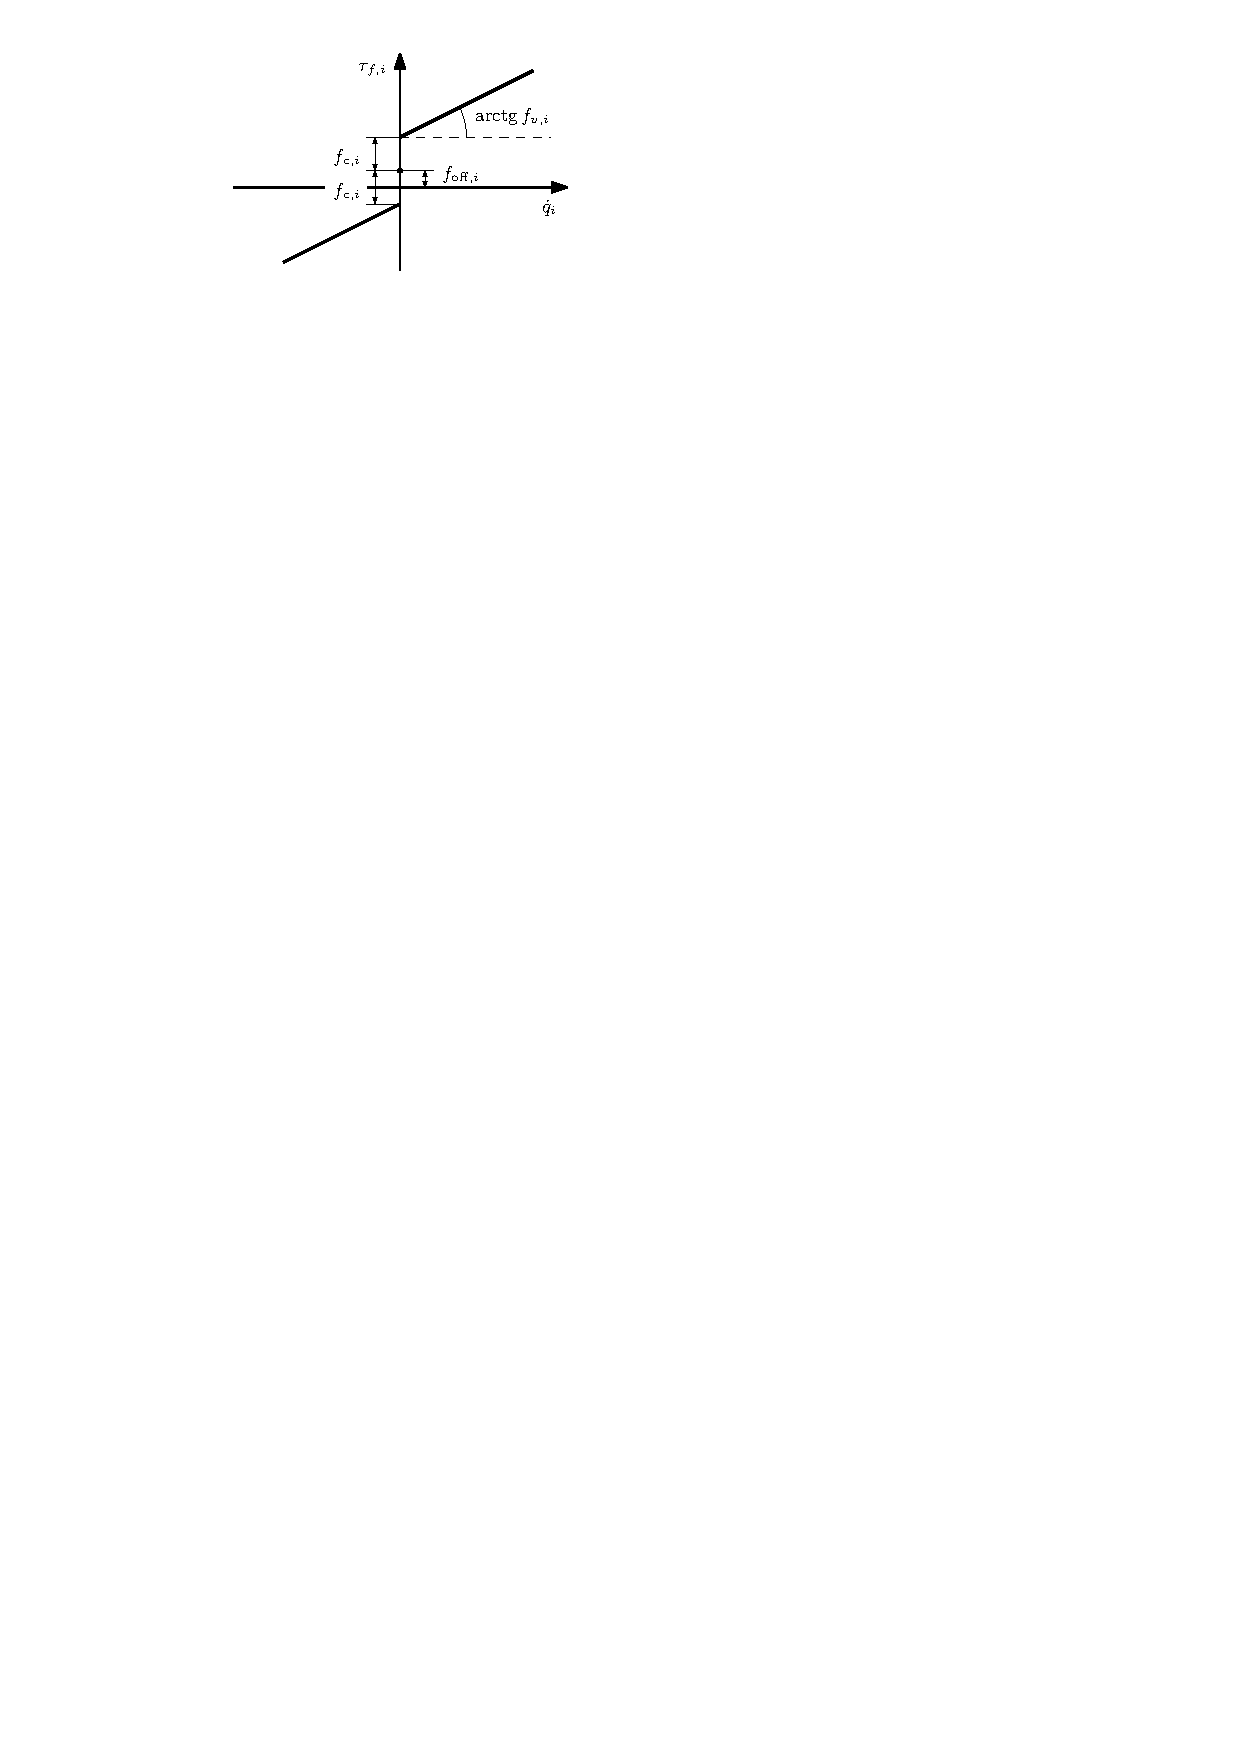
\includegraphics[width=0.7\textwidth]{friction_torque.pdf}
	\caption{График, поясняющий выбранную модель трения}
	\label{img_friction_torque}
\end{figure}

С~учетом динамики приводов и уравнения~\eqref{simple_dynamics} можно окончательно получить модель манипулятора:
\begin{equation}\label{eq_model_with_standard_matrix}
\tau_e = M(q) \ddot{q} + C(q,\dot{q}) \dot{q} + G(q) + t_f(\dot{q}),
\end{equation}
где $M(q) = I_a + D(q)$.


\subsubsection{Идентификация динамических параметров}
Динамические характеристики робота с необходимой для расчетов точностью не определены, а некоторые, такие как параметры трения, вообще неизвестны. В связи с этим необходимо решить задачу идентификации.

\textbf{Линейная регрессионная модель манипулятора}

Для проведения процедуры идентификации динамических параметров манипулятора необходимо представить динамическую модель в регрессионной форме. Для этого, используя выражение для кинетической и потенциальной энергий, нужно найти функцию Лагранжа:

\begin{gather}
L = K - U = \notag
\\
= \sum_{i=1}^5 \Biggl( m_i \left( \frac{1}{2} (v^i_i)^T v^i_i + g_i^T r^i_{0,\,i} \right) + (m_ir^i_{i,\,ci})^T \cdot \left( v^i_i \times \omega^i_i + g_i \right) + \frac{1}{2} (\omega^i_i)^T \mathcal{I}^{i}_i \omega^i_i \Biggr) = \notag
\\
= \sum_{i=1}^5 \Biggl( m_i \underbrace{\left( \frac{1}{2} (v^i_i)^T v^i_i + g_i^T r^i_{0,\,i} \right)}_{\ds L_{i,1}} + m_i x_{ci} \cdot \underbrace{x\left\{ v^i_i \times \omega^i_i + g_i \right\}}_{\ds L_{i,2}} + \notag
\\
+ m_i y_{ci} \cdot \underbrace{y\left\{ v^i_i \times \omega^i_i + g_i \right\}}_{\ds L_{i,3}} + m_i z_{ci} \cdot \underbrace{z\left\{ v^i_i \times \omega^i_i + g_i \right\}}_{\ds L_{i,4}} + I_{i,\,xx} \cdot \underbrace{\frac{1}{2} \cdot \bigl(x\{\omega^i_i\}\bigr)^2}_{\ds L_{i,5}} +\notag
\\
+ I_{i,\,yy} \cdot \underbrace{\frac{1}{2} \cdot \bigl(y\{\omega^i_i\}\bigr)^2}_{\ds L_{i,6}} + I_{i,\,zz} \cdot \underbrace{\frac{1}{2} \cdot \bigl(z\{\omega^i_i\}\bigr)^2}_{\ds L_{i,7}} + I_{i,\,xy} \cdot \underbrace{x\{\omega^i_i\} \cdot y\{\omega^i_i\}}_{\ds L_{i,8}} +\notag
\\
+ I_{i,\,xz} \cdot \underbrace{x\{\omega^i_i\} \cdot z\{\omega^i_i\}}_{\ds L_{i,9}} + I_{i,\,yz} \cdot \underbrace{y\{\omega^i_i\} \cdot z\{\omega^i_i\}}_{\ds L_{i,10}}\Biggr) \ldotp
\end{gather}

Уравнения движения робота:
\begin{equation}
\frac{d}{dt}\frac{\partial L}{\partial\dot{q_i}} - \frac{\partial L}{\partial q_i} = \tau_i, \quad i = \overline{1,5} \qquad \Rightarrow
\end{equation}
\begin{equation}
\Rightarrow \quad
\left\{
\begin{aligned}
\!&\sum_{i=1}^5 \bigl( m_i \cdot \mathcal{L}_1 \{L_{i,1}\} + m_i x_{ci} \cdot \mathcal{L}_1 \{L_{i,2}\} + \ldots + I_{i,\,yz} \cdot \mathcal{L}_1 \{L_{i,10}\} \bigr) = \tau_1\\
\!&\sum_{i=1}^5 \bigl( m_i \cdot \mathcal{L}_2 \{L_{i,1}\} + m_i x_{ci} \cdot \mathcal{L}_2 \{L_{i,2}\} + \ldots + I_{i,\,yz} \cdot \mathcal{L}_2 \{L_{i,10}\} \bigr) = \tau_2\\
\!&\ldots\\
\!&\sum_{i=1}^5 \bigl( m_i \cdot \mathcal{L}_5 \{L_{i,1}\} + m_i x_{ci} \cdot \mathcal{L}_5 \{L_{i,2}\} + \ldots + I_{i,\,yz} \cdot \mathcal{L}_5 \{L_{i,10}\} \bigr) = \tau_5
\end{aligned}
\right.
\end{equation}
где $\mathcal{L}_j$~--- оператор, работающий в соответствии с формулой:
\begin{equation}
\mathcal{L}_j : \quad \mathcal{L}_j \{f\} = \frac{d}{dt}\frac{\partial f}{\partial\dot{q_j}} - \frac{\partial f}{\partial q_j},
\end{equation}
где в свою очередь $f = f(\dot{q}(t), q(t))$.
Если же заметить, что
\begin{equation}
\mathcal{L}_j \{L_{i,k}\} = 0 \qquad \text{при }j > i, \quad i,j=\overline{1,5}, \quad k=\overline{1,10},
\end{equation}
то выражения для них упрощаются до:
\begin{equation}
\left\{
\begin{aligned}
\!&\sum_{i=1}^5 \bigl( m_i \cdot \mathcal{L}_1 \{L_{i,1}\} + m_i x_{ci} \cdot \mathcal{L}_1 \{L_{i,2}\} + \ldots + I_{i,\,yz} \cdot \mathcal{L}_1 \{L_{i,10}\} \bigr) = \tau_1\\
\!&\sum_{i=2}^5 \bigl( m_i \cdot \mathcal{L}_2 \{L_{i,1}\} + m_i x_{ci} \cdot \mathcal{L}_2 \{L_{i,2}\} + \ldots + I_{i,\,yz} \cdot \mathcal{L}_2 \{L_{i,10}\} \bigr) = \tau_2\\
\!&\ldots\\
\!& m_5 \cdot \mathcal{L}_5 \{L_{5,1}\} + m_5 x_{c5} \cdot \mathcal{L}_5 \{L_{5,2}\} + \ldots + I_{5,\,yz} \cdot \mathcal{L}_5 \{L_{5,10}\} = \tau_5
\end{aligned}
\right.
\end{equation}
или в матричном виде
\begin{equation}\label{eq_dynamic_in_linear}
\tau = \xi \chi,
\end{equation}
где $\tau = [\tau_1, \: \tau_2, \: \ldots, \: \tau_5]^T$~--- вектор обобщенных моментов,\\ $\chi=[\chi_1, \: \chi_2, \: \ldots, \: \chi_5]^T \in \mathbb R^{50}$~--- вектор параметров робота, где в свою очередь
\begin{equation}
\chi_i =
\begin{bmatrix}
m_i & m_i x_{ci} & m_i y_{ci} & m_i z_{ci} & I_{i,\,xx} & I_{i,\,yy} & I_{i,\,zz} & I_{i,\,xy} & I_{i,\,xz} & I_{i,\,yz}
\end{bmatrix}^T\!\!\!\!;
\end{equation}
$\xi$~--- так называемый регрессор, равный
\begin{equation}
\xi =
\begin{bmatrix}
\xi_{1,1} & \xi_{1,2} & \cdots & \xi_{1,5} \\
O_{1 \times 10} & \xi_{2,2} & \cdots & \xi_{2,5} \\
\vdots & \vdots & \ddots & \vdots \\
O_{1 \times 10} & O_{1 \times 10} & O_{1 \times 10} & \xi_{5,5}
\end{bmatrix}\!\!,
\end{equation}
где в свою очередь $O_{1 \times 10}$~--- вектор-строка, состоящая из 10 нулей, а $\xi_{j,i} =$\linebreak $= \xi_{j,i}(\ddot{q}, \dot{q}, q)$~--- вектор-строка, рассчитываемый по формуле
\begin{equation}
\xi_{j,i} =
\begin{bmatrix}
\mathcal{L}_j \{L_{i,1}\} & \mathcal{L}_j \{L_{i,2}\} & \ldots & \mathcal{L}_j \{L_{i,10}\}
\end{bmatrix}\!\!\ldotp
\end{equation}

Подставляя~\eqref{eq_friction_torque} в~\eqref{eq_eqs_with_tau_f}, получим
\begin{equation}
\tau_e = I_a \ddot{q} + \xi \chi + f_v \dot{q} + f_c \sign(\dot{q}) + f_\text{off}\ldotp
\end{equation}
Если ввести в рассмотрение новые матрицы $\bar{\chi}=[\bar{\chi}_1, \: \bar\chi_2, \: \ldots, \: \bar\chi_5]^T$ и\linebreak
\begin{equation}
\bar\xi =
\begin{bmatrix}
\bar\xi_{1,1} & \bar\xi_{1,2} & \cdots & \bar\xi_{1,5} \\
O_{1 \times 10} & \bar\xi_{2,2} & \cdots & \bar\xi_{2,5} \\
\vdots & \vdots & \ddots & \vdots \\
O_{1 \times 10} & O_{1 \times 10} & O_{1 \times 10} & \bar\xi_{5,5}
\end{bmatrix}\!\!,
\end{equation}
определяемые выражениями
\begin{equation}
\bar{\chi}_i =
\begin{bmatrix}
\chi_i & I_{a,i} & f_{v,i} & f_{c,i} & f_{\text{off},i}
\end{bmatrix}^T\!\!\!\!,
\end{equation}
\begin{equation}
\bar{\xi}_{j,i} =
\left\{
\begin{aligned}
\!\begin{bmatrix}\xi_{j,i} & 0 & 0 & 0 & 0\end{bmatrix}&, && i \ne j \\
\!\begin{bmatrix}\xi_{j,i} & \ddot{q_j} & \dot{q_j} & \sign(\dot{q_j}) & 1\end{bmatrix}&, &&i = j
\end{aligned}
\right.
\end{equation}
то данное выражение может быть записано в следующем матричном виде:
\begin{equation}\label{eq_extended_dynamic_in_linear}
\tau_e = \bar\xi \bar\chi \ldotp
\end{equation}





\subsubsection{Система динамического управление}\label{part_dynamic_control}

Каждый из приводов манипулятора робота Kuka Youbot имеет собственную систему управления, структура которой иллюстрируется схемой с рисунка~\ref{img_structure_of_actuator_cs}.
Из нее видно, что каждый из приводов робота может управляться заданием значения для угла~$q_{di}$, или скорости~$\dot{q}_{di}$, или момента силы $\tau_{ed,i}$, который должен быть на нем обеспечен.
Это значение подается на вход соответствующего ПИД-регулятора, коэффициенты которого доступны настройке, и далее (уже в виде сигнала напряжения $u$)~--- на контролируемый двигатель.

\vspace{0.5cm}

\begin{figure}[h!]
	\centering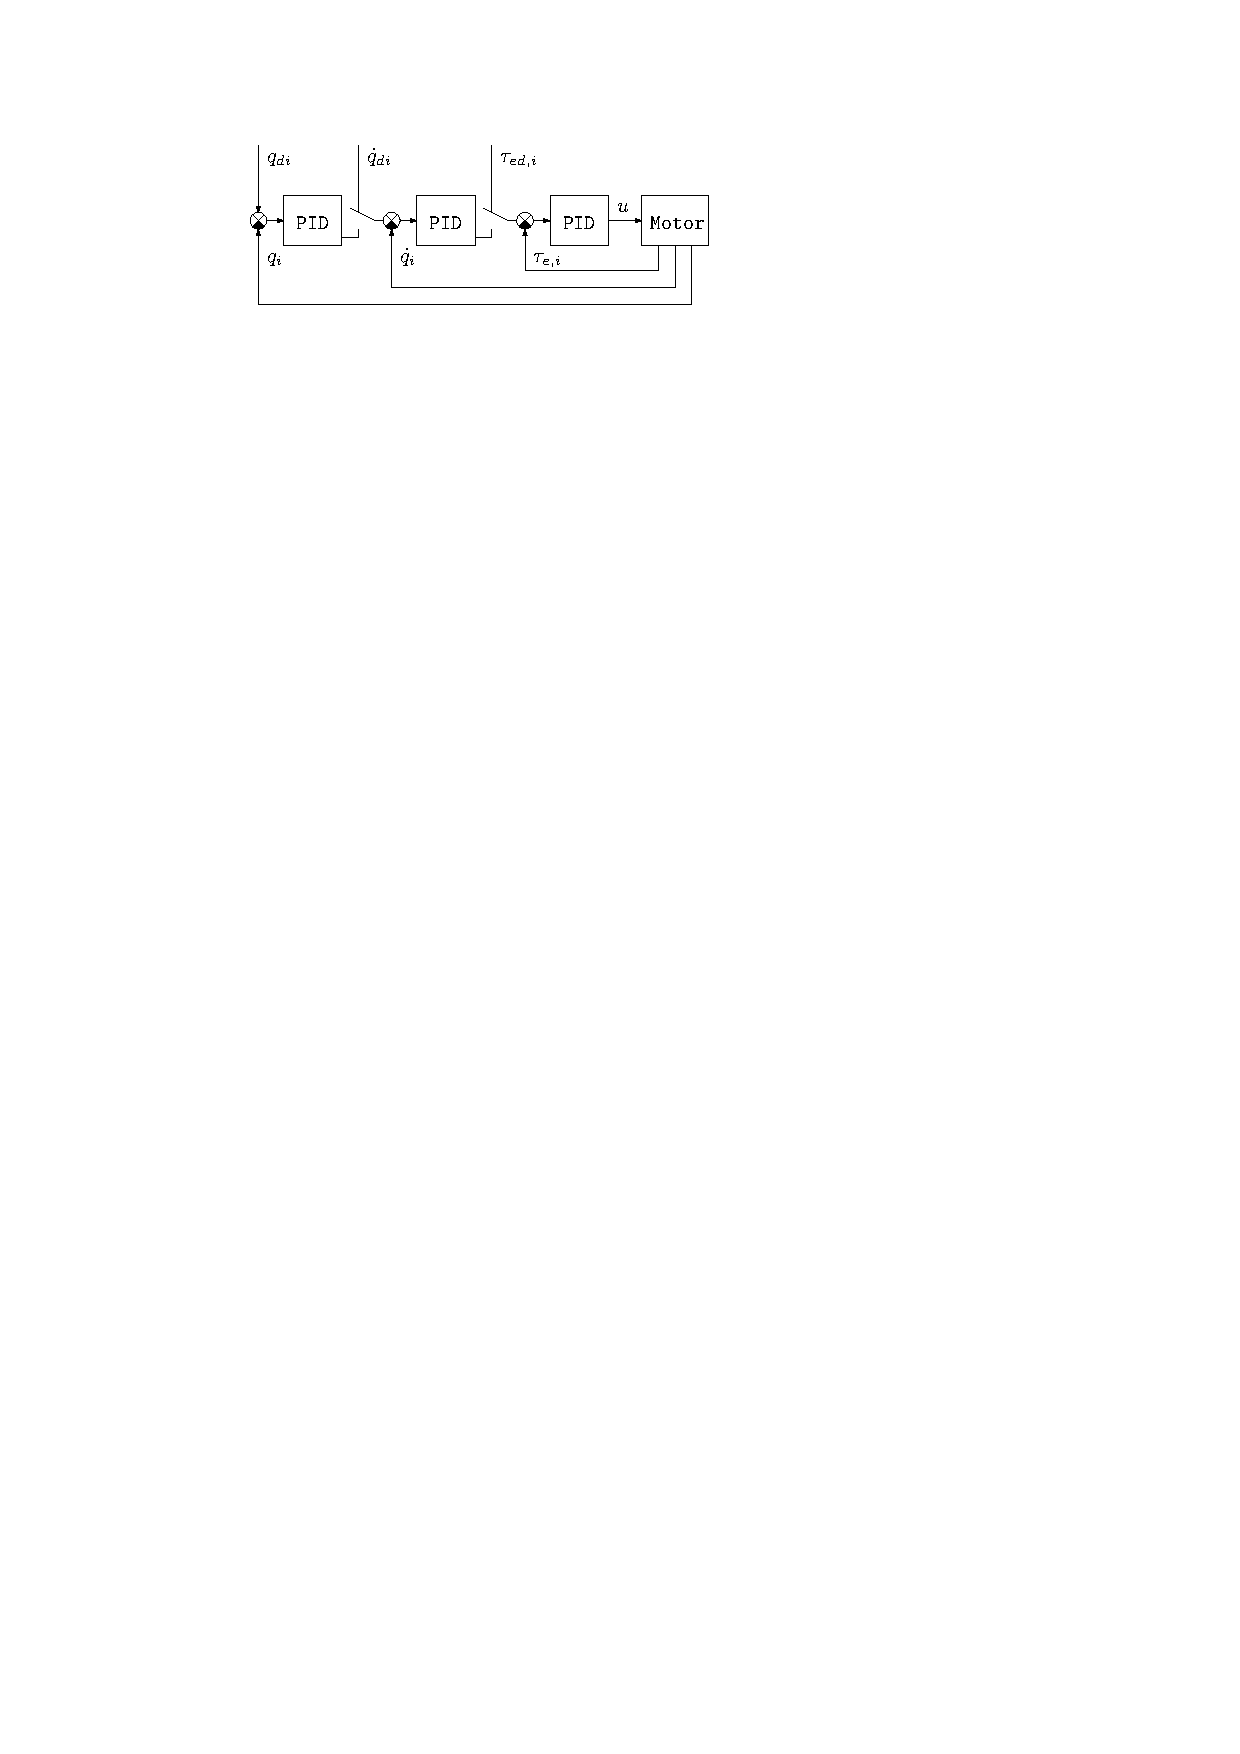
\includegraphics[width=0.8\textwidth]{structure_of_actuator_cs.pdf}
	\caption{Структура системы управления, контролирующей работу каждого из приводов робота.}
	\label{img_structure_of_actuator_cs}
\end{figure}

Далее в тексте документа будут рассмотрены системы управления, в которых в качестве управляющего сигнала рассматривается вектор $\tau_e(t)$.
При этом будет предполагаться, что задаваемые значения для моментов сил достигаются на двигателях мгновенно.
Такое предположение будем считать возможным по той причине, что процессы в контуре момента в рассмотренной выше системе управления характеризуются малыми временами переходных процессов.
В~качестве иллюстрации к сказанному можно привести рисунок~\ref{img_pid_transition_function}.
На нем показан график переходной функции системы управления моментом силы, развиваемым приводом i-го звена.

Из величин, описывающих состояние робота в данный момент времени, в используемом ПО доступны вектора $q(t)$, $\dot{q}(t)$ и $\tau_e(t)$.


\textbf{Система управления для принятия определенной конфигурации}

Для системы управления процессом принятия роботом желаемой конфигурации, описываемой вектором $q_d = \left[ q_{d1} \; q_{d2} \; q_{d3} \; q_{d4} \; q_{d5} \right]^T = const$, выберем следующий закон управления:
\begin{equation}\label{eq_set_point_control_law}
    \tau_e = K_p (q_d - q) - K_d \dot{q} + G(q) + t_f(\dot{q}),
\end{equation}
где $K_p = \diag\{k_{pi}\} = const$ и $K_d = \diag\{k_{di}\} = const$, при этом $k_{pi}>0$ и $k_{di}>0$ для $\forall i=\overline{1,5}$.
С~учетом его и уравнения~\eqref{eq_model_with_standard_matrix} модель замкнутой системы примет вид:
\begin{equation}
    M(q) \ddot{q} + C(q,\dot{q}) \dot{q} = K_p (q_d - q) - K_d \dot{q}\ldotp
\end{equation}
Это выражение с использованием обозначений
\begin{equation}
    e = q - q_d,
    \qquad \qquad
    x =
    \begin{bmatrix}
        e \\ \dot{q}
    \end{bmatrix}\!\!,
\end{equation}
можно переписать следующим образом
\begin{equation}\label{eq_controlled_object_model}
    \dot{x} = f(x),
\end{equation}
где
\begin{equation}
    f(x) =
    \begin{bmatrix}
        \dot{q} \\
        -M^{-1}(e) \Bigl( K_p e + K_d \dot{q} + C(e,\dot{q}) \dot{q} \Bigr)
    \end{bmatrix}\!\!\ldotp
\end{equation}

Заметим, что равновесным состоянием системы~\eqref{eq_controlled_object_model} является точка \linebreak $x_0 = [0\;0\;\ldots\;0]^T$, так как $f(x_0) = [0\;0\;\ldots\;0]^T$.

Рассмотрим следующую функцию Ляпунова:
\begin{equation}
    V(x) = \frac{1}{2} \, \dot{q}^T \! M(e) \dot{q} + \frac{1}{2} \, e^T \! K_p e \ldotp
\end{equation}
Ее производная по времени\footnote{В~представленных ниже выкладках учтен тот факт, что матрица \linebreak $\bigl( 0.5 M(q) \bigr)^\centerdot \!\! - C(q,\dot{q})$ является кососимметричной.}
\begin{gather}
    \frac{d}{dt} V(x) = \dot{q}^T \! M(e) \ddot{q} + \dot{q}^T \frac{d}{dt} \Bigl( \frac{1}{2} M(e) \Bigr) \dot{q} + \dot{e}^T K_p e = \notag \\
    %
    = \dot{q}^T \Bigl( \tau_e - C(q,\dot{q}) \dot{q} - G(q) - t_f(\dot{q}) \Bigr) + \dot{q}^T \frac{d}{dt} \Bigl( \frac{1}{2} M(q) \Bigr) \dot{q} + \dot{q}^T K_p e  = \notag\\
    %
    = \dot{q}^T \Bigl( \tau_e - G(q) - t_f(\dot{q}) + K_p e\Bigr) + \dot{q}^T \biggl( \frac{d}{dt} \Bigl( \frac{1}{2} M(q) \Bigr) - C(q,\dot{q}) \biggr) \dot{q} = \notag \\
    %
    = \dot{q}^T \Bigl(K_p (q_d - q) - K_d \dot{q} + G(q) + t_f(\dot{q}) - G(q) - t_f(\dot{q}) + K_p (q - q_d) \Bigr) = \notag \\
    %
    = -\dot{q}^T K_d \dot{q} < 0
\end{gather}
при $x \ne x_0$ и равна нулю при $x = x_0$.
Следовательно, по 2-ой теореме Ляпунова состояние системы $x = x_0$, при котором, к слову сказать, $q = q_d$ и $\dot{q} = [0\;0\;\ldots\;0]^T$, является асимптотически устойчивым.

\textbf{Система управления процессом следования по траектории}

Для системы управления процессом следования роботом по траектории, описываемой вектор-функцией $q_d(t) = \left[ q_{d1}(t) \; q_{d2}(t) \; q_{d3}(t) \; q_{d4}(t) \; q_{d5}(t) \right]^T$\!\!\!,\; возьмем следующий закон управления:
\begin{equation}\label{eq_trajectory_tracking_control_law}
    \tau_e = M(q) \bigl( \ddot{q}_d + K_d (\dot{q}_d - \dot{q})+  K_p (q_d - q) \bigr) + C(q,\dot{q}) \dot{q} + G(q) + t_f(\dot{q}),
\end{equation}
где $K_d = const$ и $K_p = const$.

С~учетом его и уравнения~\eqref{eq_model_with_standard_matrix} модель замкнутой системы опишется следующим выражением:
\begin{equation}
    M(q) \bigl( \ddot{q}_d - \ddot{q} + K_d (\dot{q}_d - \dot{q})+  K_p (q_d - q) \bigr) = 0,
\end{equation}
которое после деления на $M(q)$ и применения обозначения
\begin{equation}
    \varepsilon = q_d - q
\end{equation}
может быть переписано в виде:
\begin{equation}\label{eq_trajectory_tracking_closed_loop}
    \ddot{\varepsilon} + K_d \dot{\varepsilon} +  K_p \varepsilon = 0 \ldotp
\end{equation}

Согласно последнему уравнению, использование закона управления~\eqref{eq_trajectory_tracking_control_law} дает возможность полностью определять поведение робота значениями матриц $K_p$ и $K_d$.

В~данной работе матрицы $K_p$ и $K_d$ были выбраны диагональными:
\begin{equation}
    K_p = \diag\{k_{pi}\},
    \qquad
    K_d = \diag\{k_{di}\},
\end{equation}
потому что это позволяет <<разбить>> уравнение~\eqref{eq_trajectory_tracking_closed_loop} на 5~независимых дифференциальных уравнений, а их компоненты~--- положительными:
\begin{equation}
    \qquad
    k_{pi} > 0,\ k_{di} > 0,\ \forall i=\overline{1,5},
\end{equation}
так как при этом система получается устойчивой (все 5~уравнений получаются имеющими корни только с отрицательной вещественной частью).

\newpage



%\subsection{Планирование движения}
%Необходимо выбрать траекторию движения схвата манипулятора такую, чтобы законы изменения положения, скоростей и ускорения, с одной стороны, соответствовали параметрам движения конвейера, а с другой~--- возможностям манипулятора.




\clearpage\newpage
\section{Планирование траекторий движения манипулятора}\label{part_trajectory}
%%% http://www-lar.deis.unibo.it/people/cmelchiorri/foundations_robotics.html

Рассматриваются задачи планирования траекторий движения манипулятора в  решении комплексных задач: перемещению в рабочем пространстве и взаимодействию с целевыми объектами.

\subsection{Постановка и описание задачи}

Успешность захвата манипулятором, перемещающегося по конвейеру объекта заключается, как в качественной работе системы управления манипулятором, так и в планировании траектории движения его схвата, которая в точности должна повторять движение объекта.

Планирование траектории подразумевает получение программной зависимости перемещения звеньев манипулятора $ \mathbf{q}(t) $ или схвата $ \mathbf{s}(t) $ на интервале $ t \in [t_s, t_f] $. Тут $ \mathbf{q} = [q_1, q_2, \dots, q_n]^T$~--- вектор обобщенных координат, $ \mathbf{s} = [x,y,z, \varphi, \psi, \theta]^T $~--- вектор положения схвата относительно базовой СК $ Ox_0y_0z_0 $.

Необходимо спланировать траектории в пространстве обобщенных координат: для задания необходимой конфигурации робота~--- удобная ориентации камеры, закрепленной на последнем звене манипулятора (перевод из точки в точку); для обхода последовательности точек~--- осознанное перемещения объекта в рабочем пространстве от конвейера в зону погрузки. Недостатком такого подхода является то, что такие траектории нельзя использовать в операциях, где задача движения формулируется в пространстве координат схвата.

Также, необходимо спланировать траекторию в пространстве координат схвата для выполнения захватывания движущегося по конвейеру объекта.

Очевидно, что манипулятор с количеством степеней свободы $ N < 6 $ ограничен в своих движениях и, как видно из рассмотренной ранее кинематики манипулятора KUKA YouBot, он не может занимать любые необходимые ориентации, из чего следует, что в задаче решаемой в этой работе конвейер необходимо располагать параллельно плоскости OXY СК $ Ox_{0}y_{0}z_{0} $.

Также заметим, что рабочая область манипулятора при схвате сориентированном перпендикулярно плоскости OXY СК $ Ox_{0}y_{0}z_{0} $ (или, что тоже самое, рабочей плоскости конвейера) существенно ограничена. На рисунке~\ref{img:work_space_noraml} зеленым выделена рабочая область, в которой возможен захват объектов с конвейера или любой другой плоскости, удовлетворяющих условию параллельности описанному выше.

%Далее рабочую область с рисунка~\ref{img:work_space_noraml} будем называть нормальной рабочей областью.

\begin{figure}[h!]
	\centering\includegraphics[width=0.8\textwidth]{ipe/ws.pdf}
	\vspace{0.5cm}
	\caption{Рабочая область манипулятора робота KUKA Youbot при ориентации схвата перпендикулярной плоскости OXY СК $ Ox_{0}y_{0}z_{0} $ с учетом ограничений по допустимым углам поворотов сочленений и зоной безопасности в виде цилиндра вокруг оси $ z_0 $ c радиусом R и высотой H}
	\label{img:work_space_noraml}
\end{figure}

Запишем последовательность действий, необходимую для захвата объекта с конвейера:
\begin{enumerate}
	\item привести манипулятор в положения для работы СТЗ;
	\item перевести манипулятор в точку пересечения траектории движения объекта по конвейеру с нормальной рабочей областью манипулятора (точка $ p_0 $ на рисунке~\ref{img:ws_and_conveyer.pdf});
	\item провести манипулятор по траектории, совпадающей с траекторией движения объекта по конвейеру~\footnote{Эта траектория представляет из себя кривую расположенную над движущимся объектом. Т.е. манипулятор следует за объектом на некотором расстоянии над ним, пока не выровняются их скорости, после чего схват опускается на высоту объекта, захватывает объект и поднимается на прежнее расcтояние.};
	\item захватить объект;
	\item перенести объект в зону для складывания объектов с конвейера.
\end{enumerate}

%%% добавить рисунок с линейным конвейером АААААА Я НЕ УСПЕЛ((9
\begin{figure}[h!]
	\centering\includegraphics[width=0.55\textwidth]{ipe/ws_and_conveyer.pdf}
	\vspace{0.5cm}
	\caption{Пересечение плоскости конвейра и рабочей области манипулятора}
	\label{img:ws_and_conveyer.pdf}
\end{figure}


\subsection{Распределение допустимых скоростей в рабочем пространстве}

Необходимо выбрать траекторию движения схвата манипулятора такую, чтобы законы изменения положения, скоростей и ускорения, с одной стороны, соответствовали параметрам движения конвейера, а с другой~--- возможностям манипулятора.

Ограничения по скоростям в сочленениях заданы константами $ C_i $:
\begin{equation}\label{constrs}
|\dot{q}| \le C_i, \quad i = \overline{1,n}.
\end{equation}

Соотношения~\eqref{constrs} задают область допустимых скоростей в пространстве обобщенных координат. Скорости схвата рассчитывается из соотношений~\eqref{Jv1}--\eqref{Jw1} для решения прямой задачи о скорости и определяют отображение области допустимых скоростей в сочленениях в трехмерную область допустимых скоростей $ \bm{v}_n $, которую можно найти для каждой точки рабочего пространства. Определяя такие отображения для заданных всех возможных вариантов вектора $ \bm{q} $ можно найти распределение допустимых скоростей схвата в рабочем пространстве.

В практической реализации ограничимся получением оценки снизу и сверху значений скорости $ \bm{v}_n $ в рабочей зоне. Для этого определим евклидову норму вектора скорости $ \bm{v}_n $:
\begin{equation}
||\bm{v}_n|| = (\bm{v}^T \cdot \bm{v})^{\frac{1}{2}} = (\dot{\bm{q}}^T \cdot J_v^T(\bm{q}) \cdot J_v(\bm{q}) \cdot  \dot{\bm{q}})^{\frac{1}{2}}
\end{equation}
Тогда, обозначив за минимальное $ \underline{\lambda}(q) $ и максимальное $ \overline{\lambda}(q) $ характеристические числа матрицы $  J_v^T(\bm{q}) \cdot J_v(\bm{q}) $ и на основании свойств квадратичных форм, запишем:
\begin{equation}
\underline{\lambda}(q) \cdot ||\dot{\bm{q}}||^2 \le || \bm{v}_n ||^2 \le \overline{\lambda}(q) \cdot ||\dot{\bm{q}}||^2,
\end{equation}

Окончательно, для ограничения скоростей движения схвата сверху, оценка имеет вид:
\begin{equation}
||\bm{v}_n(q)|| \le \sqrt{\overline{\lambda}(q)} \cdot ||\dot{\bm{q}}|| < \sqrt{\overline{\lambda}(q)} \cdot C,
\end{equation}
где $ C = \sqrt{\sum_{i=1}^{n} C_i^2(q)} $.

Полученная оценка не может быть найдена в вырожденных конфигурациях манипулятора, а также на границах рабочей области.


%%%%%%%%%%%%%%%%%%%%%%%%%%%%%%%%%%%%%%%%%%%%%
%%%%%%%%%%%%%%%%%%%%%%%%%%%%%%%%%%%%%%%%%%%%%
%%%%%%%%%%%%%%%%%%%%%%%%%%%%%%%%%%%%%%%%%%%%%
\subsection{Планирование траектории в пространстве обобщенных координат}

Рассмотрим движение манипулятора из точки в точку, затем расширим это решение на движение через заданную последовательность точек.


%%%%%%%%%%%%%%%%%%%%%%%%%%%%%%%%%%%%%%%%%%%%%
%%%%%%%%%%%%%%%%%%%%%%%%%%%%%%%%%%%%%%%%%%%%%
%%%%%%%%%%%%%%%%%%%%%%%%%%%%%%%%%%%%%%%%%%%%%
\vspace{0.5cm}
\subsubsection{Движение из точки в точку}

Движение манипулятора в пространстве обобщенных координат из точки~$ \mathbf{q}_s $ в~точку $ \mathbf{q}_f $ формулируется, как:
\begin{equation}
	\mathbf{q} = \mathbf{q}(t),\,\,t \in [t_s, t_f],
\end{equation}
при граничных условиях:
\begin{equation}
	\mathbf{q}(t_s) = \mathbf{q}_s, 
	\quad
	\mathbf{q}(t_f) = \mathbf{q}_f.
\end{equation}


Такое движение можно обеспечить используя кривую, составленную из парабол на участках разгона и торможения и прямой на участке с постоянной скоростью. Пример такой траектории изображен на рисунке~\ref{img:plp}.

\begin{figure}[h!]
	\centering\includegraphics[width=0.7\textwidth]{ipe/plp.pdf}
	\vspace{0.5cm}
	\caption{Траектория с постоянной скоростью на среднем участке}
	\label{img:plp}
\end{figure}

Введем ограничение максимальной скорости $ v = v_{des} $.
Тогда время отработки траектории из точки~$ \bm{q}_s $ в точку~$ \bm{q}_f $ можно записать:
\begin{equation}
	t_f = \cfrac{3}{2} \cdot \cfrac{\bm{q}_f - \bm{q}_s}{v}.
\end{equation}
Отсюда, время разгона (торможения) и границы ускорений:
\begin{equation}
	t_b = \cfrac{\bm{q}_s - \bm{q}_f + v * t_f}{v}, \quad a = \cfrac{v}{t_b}.
\end{equation}
Траектория раcчитывается из следующих соотношений:
\begin{align}
	\bm{q}(t) = 
	\begin{cases}
		\bm{q}_s + \cfrac{a}{2} \cdot t^2, &t_s \le t \le t_b, \\
		\bm{q}_s + \cfrac{a}{2} \cdot t^2, &t_b < t \le t_f - t_b,\\
		\bm{q}_s + \cfrac{a}{2} \cdot t^2, &t_f - t_b < t \le t_f.
	\end{cases}
\end{align}
Скорости получаем из:
\begin{align}
	\dot{\bm{q}}(t) = 
	\begin{cases}
		a  t, &t_s \le t \le t_b, \\
		v, &t_b < t \le t_f - t_b,\\
		a  t_f - a * t, &t_f - t_b < t \le t_f.
	\end{cases}
\end{align}
Ускорения:
\begin{align}
	\dot{\bm{q}}(t) = 
	\begin{cases}
		a, &t_s \le t \le t_b, \\
		0, &t_b < t \le t_f - t_b,\\
		-a  t_f - a  t, &t_f - t_b < t \le t_f
	\end{cases}
\end{align}

Для сравнения, реализуем менее примитивный способ планирования траектории с использованием полинома пятой степени. Расчёты будем производить для нормализованного времени $ t \in [0, 1] $.

Запишем полином пятой степени:
\begin{equation}\label{poly5}
	q_i(t) = a_i + b_i t + c_i t^2 + d_i t^3 + e_i t^4 + f_i t^5.
\end{equation}
Дважды продифференцируем~\eqref{poly5} по $ t $:
\begin{gather}
	\dot{q}_i{t} = b_i + 2c_i t + 3 d_i t^2 + 4 e_i t^3 + 5 f_i t^4, \\
	\ddot{q}_i{t} = 2c_i  + 6 d_i t + 12 e_i t^3 + 20 f_i t^3.
\end{gather}
Принудим полином~\eqref{poly5} и его производные подчиняться следующим условиям:
\begin{gather}\label{con1}
	q(0) = q_s, \quad q(1) = q_f, \\
	\dot{q}(0) = q'_s, \quad \dot{q}(1) = q'_f, \\
	\label{con3}
	\ddot{q}_(0) = 0, \quad \ddot{q}(q) = 0,
\end{gather}
где $ q_s, q_f $~--- точки начала и конца траектории, $ q'_s, q'_f $~--- скорости в этих точках, а ускорения полагаем равными нулю. 

В соответствии с условиями~\eqref{con1}-\eqref{con3} легко можно получить шесть уравнений с тремя неизвестными. Опустим элементарные преобразования и сразу запишем выражения для расчета коэффицентов полинома:
\begin{gather}
	a = q_s, \quad b = q'_s, \quad c = 0, \\
    d = 10 (q_f - q_s) - (6  q'_s + 4  q'_f), \\ 
    e = -15  (q_f - q_s) + (8  q'_s + 7  q'_f), \\
    f = 6  (q_f - q_s) - (3  q'_f + 3  q'_s).
\end{gather}

Для расчёта траектории запишем уравнения в матричном виде:
\begin{gather}
	Q = T C, \quad Q' = T C', \quad Q'' = T C'',
\end{gather}
где, для $ t = [t_1, t_2, \dots, t_f] $:
\begin{equation}
	T = 
	\begin{bmatrix}
		1 & t & t^2 & t^3 & t^4 & t^5 
	\end{bmatrix}\!\!,
\end{equation}
$ Q, Q', Q'' $~--- матрицы, размерности $ [m \times 6],\,\,m = \frac{t_f - t_s}{dt} $,
\begin{gather}
	C =
	\begin{bmatrix}
		a &b &c &d &e &f
	\end{bmatrix}^T,
	\quad
	C' = 
	\begin{bmatrix}
		b &0 &3 d& 4 e& 5 f& 0
	\end{bmatrix}^T,
	\\
	C'' = 
	\begin{bmatrix}
		0 &6 d &12 e &20 f &0 &0
	\end{bmatrix}^T,
\end{gather}
где все коэффициенты, представлены векторами.

%%%%%%%%%%%%%%%%%%%%%%%%%%%%%%%%%%%%%%%%%%%%%
%%%%%%%%%%%%%%%%%%%%%%%%%%%%%%%%%%%%%%%%%%%%%
%%%%%%%%%%%%%%%%%%%%%%%%%%%%%%%%%%%%%%%%%%%%%
\vspace{0.5cm}
\subsubsection{Движение через последовательность точек}

Предсказуемое движение всего манипуляционного механизма в рабочем пространстве обеспечим планированием гладкой траектории через заданные узловые точки $ q_i  $ в пространстве обобщенных координат. 

Введем обозначения:
\begin{equation}\label{knots}
	\bm{q} = 
	\begin{bmatrix}
		q_1 & q_2 & \dots & q_n
	\end{bmatrix},
	\quad
	\bm{t} =
	\begin{bmatrix}
	t_1 & t_2 & \dots & t_n
	\end{bmatrix},
\end{equation}
где $ \bm{q} $~-- вектор, составленный из узловых точек $ q_i $, $ \bm{t}$~--- вектор временных отметок~$ t_i $, в которые манипулятор должен пройти через~$ q_i $ узел, причем
\begin{equation}
	t_s = t_1 < t_2 < \dots < t_n = t_f.
\end{equation}

На рисунке~\ref{img:seq_points} показана последовательность точек в пространстве обобщенных координат.

\begin{figure}[h!]
	\centering\includegraphics[width=0.7\textwidth]{ipe/sequence_of_q.pdf}
	\vspace{0.5cm}
	\caption{Точки $ q_0, q_1, \dots, q_{n} $, через которые должен пройти манипулятор}
	\label{img:seq_points}
\end{figure}

Решим поставленную задачу, воспользовавшись одним из наиболее распространенных вариантов аппроксимации неизвестной функции~--- интерполяцией кубическими сплайнами. Разыскиваемая функция составляется из $ n-1 $ кубических сплайнов, сшитых между собой в точках $ q_i,\:i = \overline{2,n-1} $ по первой и второй производной сплайна. Дополнительно устанавливаются ограничения на скорости или ускорения в начальной и конечной точках функции.

Запишем кубический сплайн на интервале времени $ t \in [t_{i}, t_{i+1}] $:
\begin{equation}\label{splin}
	q_i(t) = a_i + b_i (t-t_i) + c_i (t-t_i)^2 + d_i (t-t_i)^3,
	\quad
	i = \overline{1,n-1},
\end{equation}
где $q_i(t)$~--- сплайн описывающий кривую между точками $ q_i $ и $ q_{i+1}$, $ a_i, b_i, c_i, d_i $~--- подлежащие расчёту коэффициенты сплайна, определяемые из дополнительных условий, $i$~--- номер сплайна.

Отсюда видно, что для описания функции проходящей через $ n $ точек, имеем $ n-1 $ уравнений и $ 4n $ неизвестных.

Примем за шаг сплайна следующее соотношение:
\begin{equation}\label{hi}
	h_i = t_{i+1} - t_i.
\end{equation}

Продифференцируем дважды сплайн~\eqref{splin} по $ t $:
\begin{gather}
	q'_i(t) = b_i + 2 c_i (t-t_i) + 3 d_i (t-t_i)^2, \\
	q''_i(t) = 2 c_i + 6 d_i (t-t_i).
\end{gather}

Используя соотношение~\eqref{hi}, запишем условия сшивания сплайнов~$ i $ и~$ (i+1) $ для~$ i = \overline{1,n-1} $:
\begin{enumerate}
	\item конец $ i $ должен совпадать с началом $ (i+1) $:
	\begin{gather}\label{condition_q}
		q_i(t_{i+1}) = q_{i+1}(t_i)
		\quad \Rightarrow \quad
		a_{i+1} = a_{i} + b_i h_i + c_i h_i^2 + d_i h_i^3.
	\end{gather}
	Имеем: $ 3n $~--- неизвестных, $ n $~--- уравнений,
	\item первые производные сплайнов в точке сшивания должны быть равны:
	\begin{gather}\label{condition_q'}
		q'_i(t_{i+1}) = q'_i+1(t_i)
		\quad \Rightarrow \quad
		b_{i+1} = b_i + 2 c_i h_i + 3 d_i h_i^2.
	\end{gather}
	Имеем: $ 3n $~--- неизвестных, $ 2n $~--- уравнений,
	\item вторые производные сплайнов в точке сшивания должны быть равны:
	\begin{gather}\label{condition_q''}
		q''_i(t_{i+1}) = q''_i+1(t_i)
		\quad \Rightarrow \quad
		c_{i+1} = c_i h_i + 3 d_i h_i,
	\end{gather}
	Имеем: $ 3n $~--- неизвестных, $ 3n $~--- уравнений.
\end{enumerate}

Для расчёта коэффициентов сплайна проведём следующие преобразования над~\eqref{condition_q}--\eqref{condition_q''}. Выразим $ d_i $ из~\eqref{condition_q''}:
\begin{equation}\label{di}
	d_i = \cfrac{c_{i+1} - c_i}{3 h_i}.
\end{equation}

Подставив~\eqref{di} в~\eqref{condition_q} и~\eqref{condition_q'} и упрастив, получим:
\begin{gather}\label{aip1}
	a_{i+1} = a_i + b_i h_i + \cfrac{h_i^2}{3} \cdot ( 2 c_i + c_{i+1} ), \\
	\label{bip1}
	b_{i+1} = b_i + h_i ( c_i + c_{i+1} ).
\end{gather}

Выразим $ b_i $ из~\eqref{aip1}:
\begin{equation}\label{bi}
	b_i = \cfrac{1}{h_i} \cdot ( a_{i+1} - a_{i} ) - \cfrac{h_i}{3} \cdot ( 2 c_i + c_{i+1} ).
\end{equation}

Уменьшив значение индекса~$i$ на единицу в~\eqref{bip1} и~\eqref{bi}, получим:
\begin{gather}
	\label{bip1_main}
	b_{i-1} = \cfrac{1}{h_{i-1}} \cdot ( a_i - a_{i-1} ) - \cfrac{h_{i-1}}{3} \cdot ( 2 c_{i-1} + c_i ), \\
	\label{bi_main}
	b_i = b_{i-1} + h_{i-1} ( c_{i-1} + c_i ).
\end{gather}

После подстановки~\eqref{bi} и~\eqref{bip1_main} в~\eqref{bi_main} и некоторых элементарных преобразований, запишем:
\begin{equation}\label{c_main}
	\underbrace{\cfrac{}{} h_{i-1}}_{\alpha_i} c_{i-1} + \underbrace{\cfrac{}{} 2 ( h_{i-1} + h_i )}_{\beta_i} c_i + \underbrace{\cfrac{}{} h_i}_{\gamma_i} c_{i+1} = \underbrace{\cfrac{3}{h_i} \cdot ( a_{i+1} - a_i ) - \cfrac{3}{h_{i-1}} \cdot ( a_i - a_{i-1} )}_{\delta_i},
\end{equation}
Отсюда видно: $ n-1 $~--- уравнений, $ n+1 $~--- неизвестных.

Добавим граничные условия, зафиксировав концы крайних сплайнов, обеспечивающие заданные первые производные~$ q'_s $ и~$ q'_f $ в точках $ t_s $ и~$ t_f $ соответственно. Используя~\eqref{bi}, получим:
\begin{align}\label{condition_CBC} % clamped boundary condition
	q'(t_s) = q'_i (t_s) = b_1 = q'_s
	\quad \Rightarrow \quad&
	h_1 (2 c_1 + c_2) = \cfrac{3}{h_1} \cdot ( a_2 - a_1 ) - 3 q'_s,\\
	q'(t_f) = q'_n (t_f) = b_n = q'_f
	\quad \Rightarrow \quad& \\ 	\quad \Rightarrow \quad
	h_{n-1} (2 c_{n} + c_{n-1}) =&  \,\,3 q'_f - \cfrac{3}{h_{n-1}} \cdot ( a_{n} - a_{n-1} ).
\end{align}

Таким образом,~$ n-1 $ уравнений~\eqref{c_main} при $ i = \overline{1,n-1} $ вместе с условиями~\eqref{condition_q}-\eqref{condition_q''} и~\eqref{condition_CBC} образуют систему линейных алгебраических уравнений для определения коэффициентов $ c_i$. Коэффициенты~$ b_i $ и~$ d_i $ рассчитываются из выражений~\eqref{di} и~\eqref{bi}, коэффициенты~$ a_i $ равны значениям аппроксимируемой функции в узлах~\eqref{knots}.

Запишем уравнения~\eqref{c_main} с учетом введенных там обозначений $ \alpha_i, \beta_i, \gamma_i$ и~$\delta_i $ в матричном виде:
\begin{equation}\label{tridiagonal_eq}
	A c = \delta,
\end{equation}
где $ A $~--- трехдиагональная матрица, содержащая кооэффициенты~$\alpha_i, \:\beta_i, \:\gamma_i$, $ c $~--- вектор разыскиваемых коэффициетов $ c_i $, $ \delta $~--- вектор, составленный из соотношений правой части уравнения~\eqref{c_main}.

Воспользуемся алгоритмом Томаса~\cite{datta2010numerical} (метод прогонки) для решения уравнения~\eqref{tridiagonal_eq}, содержащего трехдиагональную матрицу.

Перепишем выражение~\eqref{c_main} в виде:
\begin{equation}
	c_i = z_i - \mu_i \cdot c_{i+1},
\end{equation}
где прогоночные коэффициенты:
\begin{gather}\label{tomas_coefs}
	z_i = \cfrac{\delta_i - \alpha_i z_{i-1}}{\beta_i + \alpha_i \mu_{i-1}},
	\quad
	\mu_i = \cfrac{\gamma_i}{\beta_i + \alpha_i \mu_{i-1}}.
\end{gather}

Алгоритм решает уравнение за два прохода:
\begin{enumerate}
	\item Прямой ход. Рассчитываются начальные условия~\eqref{tomas_coefs} при $ \alpha_1 = 0 $:
	\begin{gather}
	\mu_1 = \cfrac{\gamma_1}{\beta_1} = \cfrac{h_1}{2 h_1} = 0.5, 
	\quad
	z_1 = \cfrac{\delta_1}{\beta_1}.
	\end{gather}
	Вычисляются прогоночные коэффициенты $ z_i, \: \mu_i $ из выражения~\eqref{tomas_coefs} для $ i = \overline{2,n-1} $,
	\item Обратный ход. Вычисляется $ z_n = c_n $.
	Вычисляются коэффициенты $ c_i $ для $ i = \overline{n-1,1} $.
\end{enumerate}

Результат работы на примере интерполяции синуса, показан на рисунке~\ref{img:cubic_splines_method_test}.
\begin{figure}[h!]
	\centering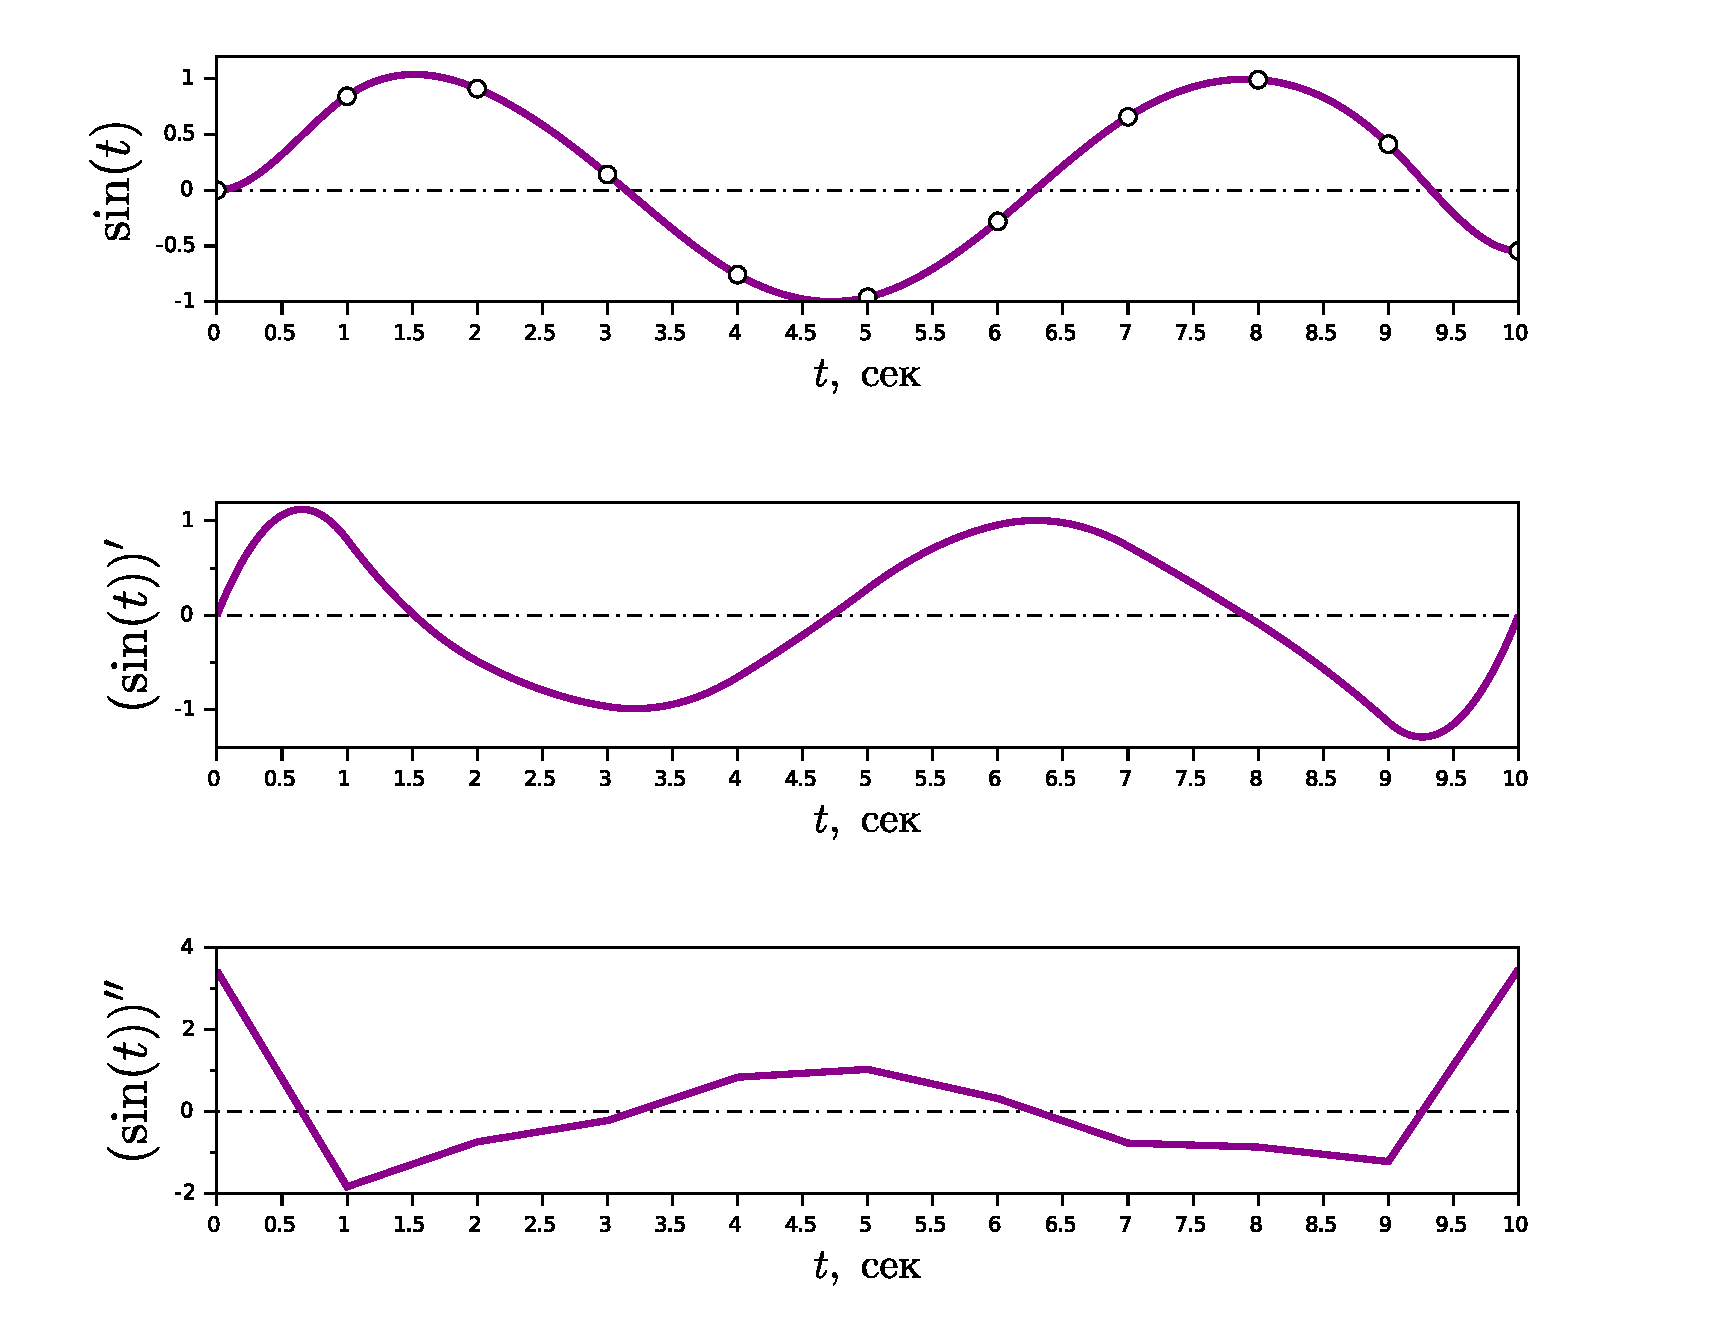
\includegraphics[width=\textwidth]{cubic_splines_examples.pdf}
	\vspace{0.5cm}
	\caption{Пример результата интерполяции набора из одиннадцати точек функции $\sin(t)$}
	\label{img:cubic_splines_method_test}
\end{figure}

Планирование траектории должно осуществляться перед началом работы. При реализации описаного метода может случиться так, что скорости и ускорения некоторых из компонентов векторов обобщенных координат будут превышать допустимые значения скоростей и ускорения, которые могут развить приводы манипулятора. Один и способов борьбы с этим~--- увеличить время прохождения траектории на участке, на котором ограничение нарушено.


%Далее, с помощью рекуррентных соотношений~\eqref{spline_equations}, \eqref{ck}, \eqref{dk} можно найти все коэффициенты $ c_k $ и $ d_k $, $ k = \overline{1,2,\dots,n} $, если принять последние соотношения в качестве начальных условий, после чего, вычислисть $ x_k $, $ k=\overline{n-1, n-2, \dots, 1} $.

%%%%%%%%%%%%%%%%%%%%%%%%%%%%%%%%%%%%%%%%%%%%%
%%%%%%%%%%%%%%%%%%%%%%%%%%%%%%%%%%%%%%%%%%%%%
%%%%%%%%%%%%%%%%%%%%%%%%%%%%%%%%%%%%%%%%%%%%%
\vspace{0.5cm}
\subsection{Планирование траектории в пространстве координат схвата}

Планирование траектории в пространстве координат схвата включает в себя два этапа: на первом этапе планируется траектория относительно базовой СК робота, на втором этапе~--- полученная траектория переводится в пространство обобщенных координат робота и трансформируется в рассмотренную выше задачу.

\begin{figure}[h!]
	\centering\includegraphics[width=1\textwidth]{ipe/trajectory_planning.pdf}
	\vspace{0.5cm}
	\caption{Планирование траекторий на конвейерах: слева~--- вращающийся стол; справа~--- линейный конвейер}
	\label{img:trajectory_planning}
\end{figure}

Для планирования траектории захвата движущегося по конвейеру объекта, получим аналитические выражения для геометрического пути следования этого объекта. 
Дальнейшие рассуждения и обозначения наглядно представлены на рисунке~\ref{img:trajectory_planning}.

Необходимо представить траекторию, как зависимость
\begin{equation}
	T = T(t),
\end{equation}
которая удовлетворяет требованиям плавного разгона и торможения, тогда
\begin{equation}\label{Tt}
	T(t) = T_0 \cdot A(\overrightarrow{n}, \delta(t), \rho(t)),
\end{equation}
где $ A(t) $ матрица однородных преобразований между точкой траектории и вектором обобщенных координат:
\begin{equation}
	A(t) = 
	\begin{bmatrix}
	R(t) & \mathbf{\rho}(t)\\
	000&1
	\end{bmatrix}\!.
\end{equation}

Заметим, что в соответствии с рисунком~\ref{img:trajectory_planning} и~\eqref{Tt}:
\begin{equation}
	T(t_0) =T_0, \quad T(t_0 + \tau) = T_0 \cdot T_f^{-1},
\end{equation}
\begin{equation}
	R(t_0) = E, \quad R(t_0+\tau) = R_0 \cdot R_f.
\end{equation}
\begin{equation}
	\rho(t_0) = 0, \quad \rho(t_0 + \tau) = R^T_0 (r_f - r_0),
\end{equation}
где $ r_0 $ и $ r_f $~--векторы переноса составленные из первых трех компонент векторов~$ \mathbf{p}_0 $ и~$ \mathbf{p}_f $.

Найдем вектор $ \overrightarrow{n} $, вокруг которого осуществляется поворот из следующих выражений:
\begin{equation}
	\delta(t_0 + \tau) = \arccos{\cfrac{r_{11} + r_{22} + r_{33} - 1}{2}},
\end{equation}
\begin{equation}
	\mathbf{n} = \cfrac{1}{2 \sin{\delta}} 
	\cdot
	\begin{bmatrix}
		r_{32} - r_{23} \\
		r_{13} - r_{31} \\
		r_{21} - r_{12}
	\end{bmatrix}\!,
\end{equation}
где $ r_{ij} $~--- элементы матрицы $ R(t_0 + \tau) $.

Окончательно, матрица поворота рассчитывается из выражения:
\begin{equation}\label{Rt}
	R(t) = \cos \delta(t) \cdot E + (1 - \cos \delta(t)) \cdot \mathbf{n} \cdot \mathbf{n}^T + \sin \delta(t) \cdot \Omega_n,
\end{equation}
где $ \Omega_n $~--- кососимметрическая матрица для вектора $ \mathbf{n} $.

Функции $ \rho(r) $ и $ \delta(t) $ выбираются исходя из условия обеспечения плавности разгона и торможения.

Для случая конвейера, представленного вращающимся столом, объект покоящийся на столе описывает окружность, закон движения по которой в плоскости параллельной плоскости OXY:
\begin{equation}
	\begin{cases}
		x(t) = R_c \cos{\theta(t)}\\
		y(t) = R_c \sin{\theta(t)} \\
		z(t) = const
	\end{cases}\!\!\!\!\!\!\!\!,
\end{equation}
где $ R_c $~--- радиус окружности, описываемой объектом при вращении стола, $ \theta(t) $~--- поворот стола.

Тогда, учитывая, что закон движения схвата манипулятора должен в точности повторять движение подвижного объекта, параметризуем закон движения схвата параметром поворота вращающегося стола $\theta = \theta(t)$, получим:
\begin{equation}
	\mathbf{p} = \mathbf{p}(\theta) = 
	\begin{bmatrix}
		R_c \cos{\theta}\\
		R_c \sin{\theta} \\
		z \\
		1
	\end{bmatrix}\!\!,
	\quad
	\theta \in [\theta_0,\,\,\theta_f].
\end{equation}

%%% the curve is regular
При этом нужно, чтобы выполнялось условие непрерывности траектории
\begin{equation}
	\dot{\mathbf{p}} = \cfrac{d \mathbf{p}}{d \theta} \ne 0,
	\quad
	\forall{\theta} \in [\theta_0,\,\,\theta_f].
\end{equation}

Траектория ориентации схвата определяется выражением~\eqref{Rt}

В этом разделе были проанализированы конфигурация и необходимая ориентация схвата в рабочем пространстве манипулятора робота KUKA Yobot. После этого были решены задачи планирования траекторий для перевода манипулятора из точки в точку, для обхода последовательности точек и для задания закона движения в пространстве координат схвата.

%\subsection{Геометрия рабочего пространства манипулятора}
%\subsubsection{Конфигурация рабочего пространства}
%\subsubsection{Анализ ориентации схвата в рабочем пространстве}

%\subsection{Кинематические свойства манипулятора}
%\subsubsection{Распределение допустимых скоростей}
%\subsubsection{Оценка мобильности и приемистости манипулятора}

\newpage



\newpage
\section{Разработка системы технического зрения}

Использование системы технического зрения (СТЗ) в разрабатываемой робототехнической системе обусловлено необходимостью наделить СУ манипулятора способностью самостоятельно выбирать свое поведение в соответствии с изменениями окружающей среды. 

СТЗ состоит из RGBD видеокамеры Intel RealSense SR300, компьютера и программного обеспечения. Камера закреплена на пятом звене манипулятора и имеет матрицу трансформации из внутренней СК камеры в СК $ Ox_{5}y_{5}z_{5} $, причем, оптическая ось камеры и $ Oz_{5} $ сонаправлены.

Технические характеристики сенсоров видеокамеры Intel RealSenseSR300 приведены в таблицах~\ref{table_gen_info_of_camera}--\ref{table_gen_info_of_camera2}, а внешний вид представлен на рисунке~\ref{img:camera}. Принцип получения карты глубины схематично изображен на рисунке~\ref{img:camera2}.

\begin{figure}[h!]
	\centering{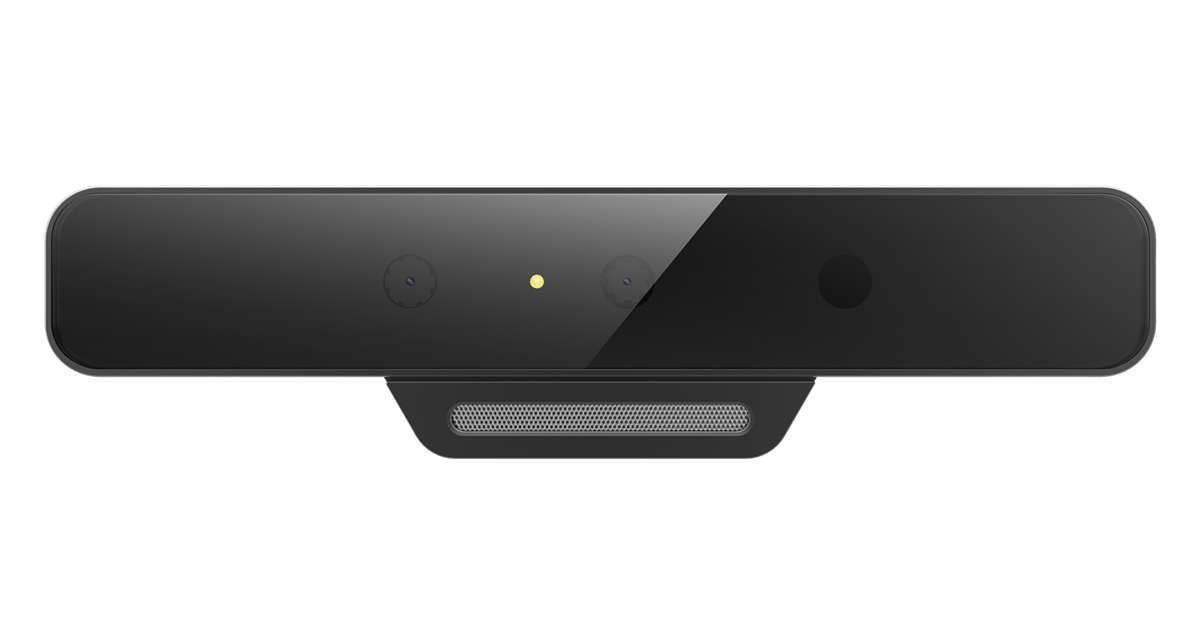
\includegraphics[width=0.4\textwidth]{rs_front.png}}
	\vspace{0.5cm}
	\caption{Внешний вид 3D-камеры Intel RealSense SR300}
	\label{img:camera}
\end{figure}

\begin{table}[h!]
	\centering\caption{Параметры инфракрасной и цветной камер RealSense~SR300}
	\label{table_gen_info_of_camera}
	\begin{tabularx}{\textwidth}{|Y|Y|Y|}
		\hline
		\multicolumn{1}{|c|}{Параметр} & ИК-камера                & RGB-камера               \\ \hline
		Разрешение, пикс               & $640 \times 480$         & $1920 \times 1080$       \\ \hline
		Вертикальный угол обзора, град   & $55 \pm 2$   & $41.5 \pm 2$ \\ \hline
		Горизонтальный угол обзора, град & $71.5 \pm 2$ & $68 \pm 2$   \\ \hline
		Диагональный угол обзора, град   & $88 \pm 3$   & $75.2 \pm 4$ \\ \hline
	\end{tabularx}
\end{table}

\begin{figure}[h!]
	\centering{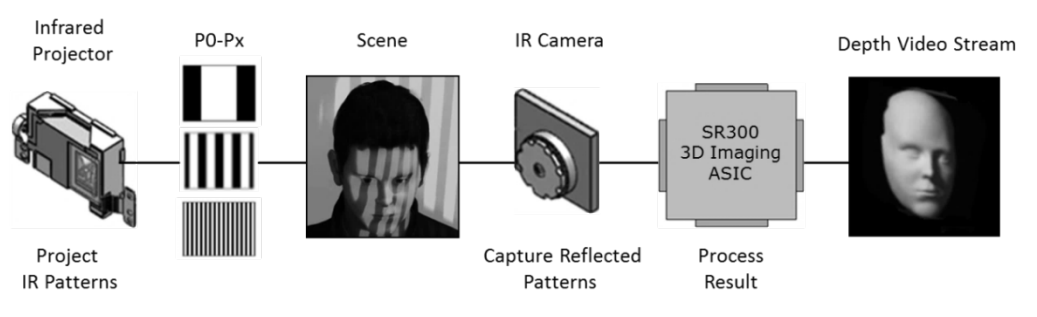
\includegraphics[width=0.9\textwidth]{sr300_depth.png}}
	\vspace{0.5cm}
	\caption{Принцип получения карты глубины}
	\label{img:camera2}
\end{figure}


\begin{table}[]
	\centering
	\caption{Параметры лазерного проектора камеры Intel~RealSense~SR300}
	\label{table_gen_info_of_camera2}
\begin{tabularx}{\textwidth}{|Y|Y|}
	\hline
	\multicolumn{1}{|c|}{Параметр} & Описание                                      \\ \hline
	Проектор                       & Структурированный свет                        \\ \hline
	Длина волны лазера, нм         & 860                                         \\ \hline
	Безопасность лазера            & Class 1                                       \\ \hline
	Вертикальный угол проекции, град     & $60 \pm 4$                        \\ \hline
	Горизонтальный угол проекции, град   & $72.5 \pm 2$ \\ \hline
\end{tabularx}
\end{table}

\subsection{Постановка и описание задачи}

Требуется оценить параметры траектории движения объекта покоящегося на вращающемся столе, пример которого представлен на рисунках~\ref{img:ws_and_conveyer.pdf}--\ref{img:trajectory_planning}. Траектория движения~--- окружность. Подлежащие оценке параметры: $ R_c $~--- радиус окружности, которую описывает объект при вращении стола, $ Oxyz $~--- СК вращающегося стола, где $Oz$~--- ось вращения, $ \bm{p}_0 $ и $ \bm{p_f} $~--- точки входа в нормальную рабочую область манипулятора и выхода из нее соответственно, а также векторы $ \bm{s}_o$ и $ \dot{\bm{s}}_o$~--- положение объекта в пространстве и скорость, выраженные в СК $ Ox_{0}y_{0}z_{0} $:
\begin{equation}
	\bm{s}_o =
	\begin{bmatrix}
		\bm{p}_o \\
		\bm{r}_o
	\end{bmatrix},
	\quad
	\dot{\bm{s}}_o =
	\begin{bmatrix}
		\bm{v}_o \\
		\bm{\omega}_o
	\end{bmatrix}\!\!.
\end{equation}
Объект представлен в лице прямоугольного параллелепипеда.

Выделим на вращающющемся столе две зоны: приближение объекта и захвата.
Тогда, сценарий работы СТЗ следующий:
\begin{enumerate}
	\item Манипулятор принимает конфигурацию, при которой в кадр камеры попадает зона приближения объекта;
	\item Проводится процедура выделения объекта из окружающей среды и  определение его геометрии, с последующим оцениванием векторов его положения $ \bm{s}_o $ и скорости $ \dot{\bm{s}}_o $;
	\item По собранной статистике о положении и ориентации объекта на столе за время $ \Delta t $, производится оценка оси вращения стола ${\overrightarrow{\bm{n}}}$ и радиуса кривизны траектории движения объекта $ R_c $.
	\item Перед тем, как закончить свою работу, СТЗ определяет точки входа $ \bm{p}_0 $ в зону захвата и выхода $ \bm{p}_f $ из нее объекта. После этого вся накопленная информация пересылается в генератор траекторий для манипулятора.
\end{enumerate}

Первый пункт рассматривается в разделе~\ref{part_kinematic_control}, последний в~\ref{part_trajectory}, а второй и третий реализуем в этом разделе. 

Прежде, чем приступить к решению поставленных задач, сделаем два замечания:
\begin{enumerate}
	\item Использование камеры Intel RealSense SR300 позволяет упростить решение поставленных задач, так как позволяет сразу работать с \textit{облаком точек}~--- набором вершин в трехмерном пространстве, координаты которых выражены в СК камеры; также, каждая точка может иметь цвет, например, в цветовой модели RGB;
	\item Работа с глубинными картами предполагает большой объем вычислений, поэтому необходим достаточно производительный компьютер.
\end{enumerate}

Непрерывно изменяющееся состояние окружающего мира~--- вращение стола, ~--- обязывает робототехническую систему работать в реальном времени, так как нет априорной информации о расположении объектов на нем. В связи с этим, необходимо найти компромисс между точностью работы системы и скоростью  вычислений обеспечивающих достаточную точность.

Как видно из таблицы~\ref{table_gen_info_of_camera}, разрешение получаемой карты глубины и, соответственно, облака точек равно $ 640 \times 480 $, что соответствует $ 307200$ точкам, представляющих из себя, в простейшем случае, структуру из трех координат положения точки и трех векторов, задающих ориентацию, т.е. в сумме, один кадр облака может содержать от четырехсот байт. При работе с частотой 30 кадров в секунду возрастает до двенадцати мегабайт. Дополнительным аргументом становится тот факт, что при уменьшении количества точек в облаке до некоторого порога, возможно добиться не худшей точности, чем при использовании всех точек. Из этих соображений имеет смысл понизить разрешение.

Среди огромного количества фильтров разной степени сложности, выберем наиболее простой, суть которого заключается в представлении облака точек в виде восьмиричного дерева~--- октодерева. Октодерево делит облако точек на октанты (воксели), каждый из которых рекурсивно делится до тех пор, пока каждая из точек не будет в отдельном октанте. Такое представление позволяет задавать разрешение облака точек простым изменением глубины октодерева~\cite{moreno2016comparative}. Пример деления представлен на рисунке~\ref{img:octree}.

\begin{figure}[h!]
	\centering{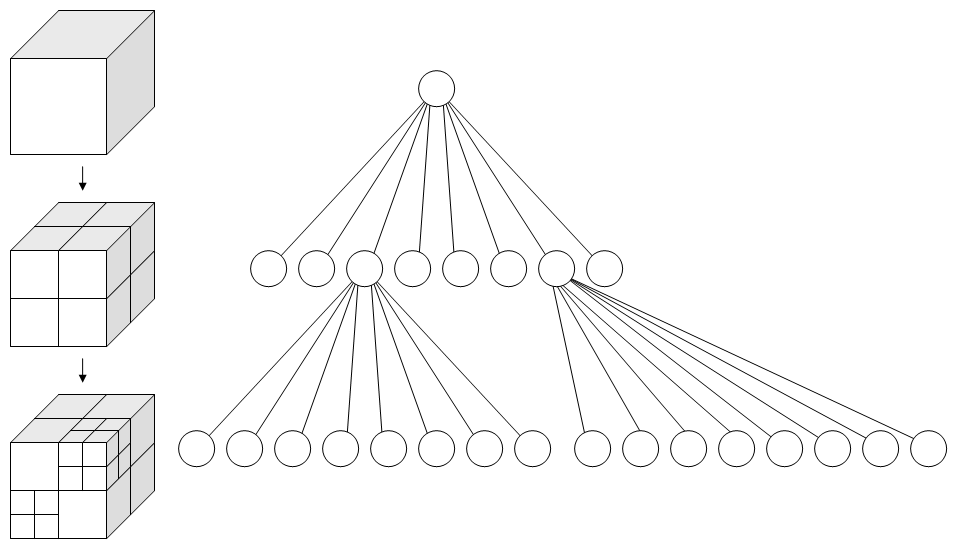
\includegraphics[width=0.7\textwidth]{octree.png}}
	\vspace{0.5cm}
	\caption{Изображение рекурсивного разделения куба на октанты и, соответствующее этому разделению, октодерево}
	\label{img:octree}
\end{figure}

Следующим этапом нужно определить плоскость вращающегося стола, на котором располагаются интересные нам объекты. Для этого воспользуемся методом оценки параметром плоскости на основе случайных выборок точек~--- RANSAC.

На вход алгоритма подается все облако точек, модель плоскости, которую нужно вписать в это болако, минимальное и максимальное число точек, которые могут входить в плоскость и максимальный разброс. На выходе получем параметры модели плоскости и точки, который входят в эту плоскость. На рисунке~\ref{img:plane} изображен пример результата работы. 

\begin{figure}[h!]
	\centering{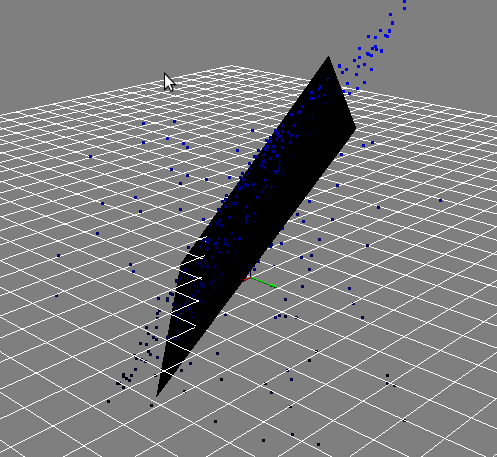
\includegraphics[width=0.7\textwidth]{plane.png}}
	\vspace{0.5cm}
	\caption{Пример вписывания плоскости в облако точек алгоритмом RANSAC}
	\label{img:plane}
\end{figure}

После определения кластера облака точек, в который входят все точки самой большой плоскости в кадре, то есть плоскости конвейера, необходимо найти объекта на этой плоскости. Для этого, построим выпуклую оболочку кластера облака точек входящих в плоскость, получив таким образом некоторый многоугольник. Далее, отбросив все точки, которе не входят в множество, включающее только внутреннюю часть призмы заданной высоты построенной на этом многоугольнике, получим все объекты расположенные на столе. В этой работе рассматривается только один объект, но это решение легко можно расширить на большее их число путем деление кластера с объектами на еще более мелкие кластеры, содержание каждый свой объект~\cite{toold3dthesis}.

Теперь, имея облако точек, включающее только целевой объект, необходимо найти его центр масс и ориентацию. Для этого воспользуемся методом определения момента инерции облака точек. Идея метода заключается в следующем. Вычисляется ковариационная матрица точечного облака и извлекаются ее собственные значения и векторы, которые представляют собой оси x, y и z, образующие ортогональный правый базис. На каждой итерации выбирается один из полученных векторов, причем вращение всегда одинаковое, что обеспечивает инвариантность к вращению всего рассматриваемого облака точек. После этого, для каждой оси рассчитывается момент инерции.

Полученные значения поворота облака точек и его центр масс будем использовать для оценки траектории движения объекта. Причем, ориентацию объекта достаточно оценить один раз, а после задавать ее дополнительное слагаемое к углу поворота вращающегося стола.

Последним этапом работы технического зрения является отслеживание траектории движения объекта и одновременная идентификация параметров этой траектории заданной в параметрической форме окружности:
\begin{equation}
\begin{cases}
	x(t) = R_c \cos{\theta(t)}\\
	y(t) = R_c \sin{\theta(t)} \\
	z(t) = const
\end{cases}\!\!\!\!\!\!\!\!,
\end{equation}
где $ R_c $~--- радиус окружности, описываемой объектом при вращении стола, $ \theta(t) $~--- поворот стола.

Таким образом, нужно найти радиус дуги, которую описывает объект при вращении стола.
Рассмотрим случай нахождения радиуса по трем известным координатам точек окружности $ A(x_1,y_1),\: B(x_2, y_2) $ и $ C(x_3, y_4) $. Возможный пример такого случая изображен на рисунке~\ref{img:circle} 

\begin{figure}[h!]
	\centering{\includegraphics[width=0.7\textwidth]{ipe/circle.pdf}}
	\vspace{0.5cm}
	\caption{Нахождение радиуса окружности по известным точкам, пренадлежащим окружности}
	\label{img:circle}
\end{figure}

Запишем уравнения для прямых $ a $ и $ b $:

\begin{gather}
	y_a = k_a (x - x_1) + y_1, \quad y_b = k_b (x - x_2) + y_2,
\end{gather}
где $ k_a$~--- коэффициент наклона прямой a, $ k_b $~--- коэффициент наклона прямой~b.

Коэффициенты рассчитываются из следующих соотношений:
\begin{equation}
	k_a = \cfrac{y_2 - y_1}{x_2 - x_1}, \quad k_b = \cfrac{y_3 - y_2}{x_3 - x_2}.
\end{equation}

Далее, найдем центр окружности, который находится на пересечении прямых проведенных через середины отрезков AB и BC. Учитывая, что коэффициент наклона перпендикулярна выражается как $ k_{a,b} = -\frac{1}{m_{a,b}}  $, запишем уравнения перпендикуляров:
\begin{equation}
	y_{\perp a} = - \cfrac{1}{k_a} \cdot \Bigg( x - \cfrac{x_1 + x_2}{2}\Bigg) + \cfrac{y_1 + y_2}{2}, \quad
	y_{\perp b} = - \cfrac{1}{k_b} \cdot \Bigg( x - \cfrac{x_2 + x_3}{2}\Bigg) + \cfrac{y_2 + y_3}{2}.
\end{equation}

И, так как полученные перпендикуляры пересекаются ровно в центре окружности, запишем для координат точки O:
\begin{gather}
	x = \cfrac{k_a k_b ( y_1 - y_3) + k_b (x1 + x2) - k_a (x_2 + x3)}{2 (k_b - k_a)},
\end{gather}
\begin{align*} 
	y = - \cfrac{1}{k_a} \cdot \Bigg( \cfrac{k_a k_b ( y_1 - y_3) + k_b (x1 + x2) - k_a (x_2 + x3)}{2 (k_b - k_a)} -\\- \cfrac{x_1 + x_2}{2} \Bigg) + \cfrac{y_1 + y_2}{2}.
\end{align*}

Имея оценку координат центра окружности, по которой двигается объект, легко найти радиус:
\begin{equation}
	R_c = \sqrt{(x - x_3)^2 + (y - y_3)^2}
\end{equation}

Таким образом, при слежении за объектом в области перед точкой $ P_0 $ для каждой полученной последовательности трех точек рассчитывается оценка радиусу. Со временем накапливаются возможные значения радиусов и координат его центра. Координаты центра следует отфильтровать, найдя центр минимальной окружности, которая охватывает большинство точек оценок координат центра траектории движения объекта.

Описанная последовательность действий позволяет определить положение и ориентацию объекта на вращающемся столе, а также момент входа объекта в область доступную для захватывания его манипулятором.

\newpage
\section{Результаты математического моделирования}

В этом разделе приводятся результаты моделирования трех главных частей робототехнической системы: планирование траекторий, управления манипулятором и системы технического зрения.

Коммуникация между всеми частями робототехнической системы реализована на базе фреймворка Robot Operation System (ROS).

Алгоритмы планирования траекторий были реализованы и отлажены в пакете прикладных математических программ Scilab. Затем реализованы в виде модуля на языке программирования C++.

Моделирование системы управления манипулятором также проводилось в Scilab. При этом использовался Robotics Toolbox~--- набор блоков для моделирования манипуляторов~\cite{roboticstoolbox}, являющийся аналогом Robotics Toolbox Питера Корка для Matlab.

Система технического зрения разрабатывалась с использованием алгоритмов обработки облаков точек Point Cloud Library (PCL). Разработка велась на языке программирования C++, результатом которой стал ros-пакет.


\subsection{Результаты планирования траектории}

Построим траектории в пространстве обобщенных координат. На рисунке~\ref{img:poses} изображены четыре выбранные конфигурации, соответствующие значениям углов поворота сочленений манипулятора, заданные векторами в~\eqref{poses_q}.
\begin{figure}[h!]
	\centering{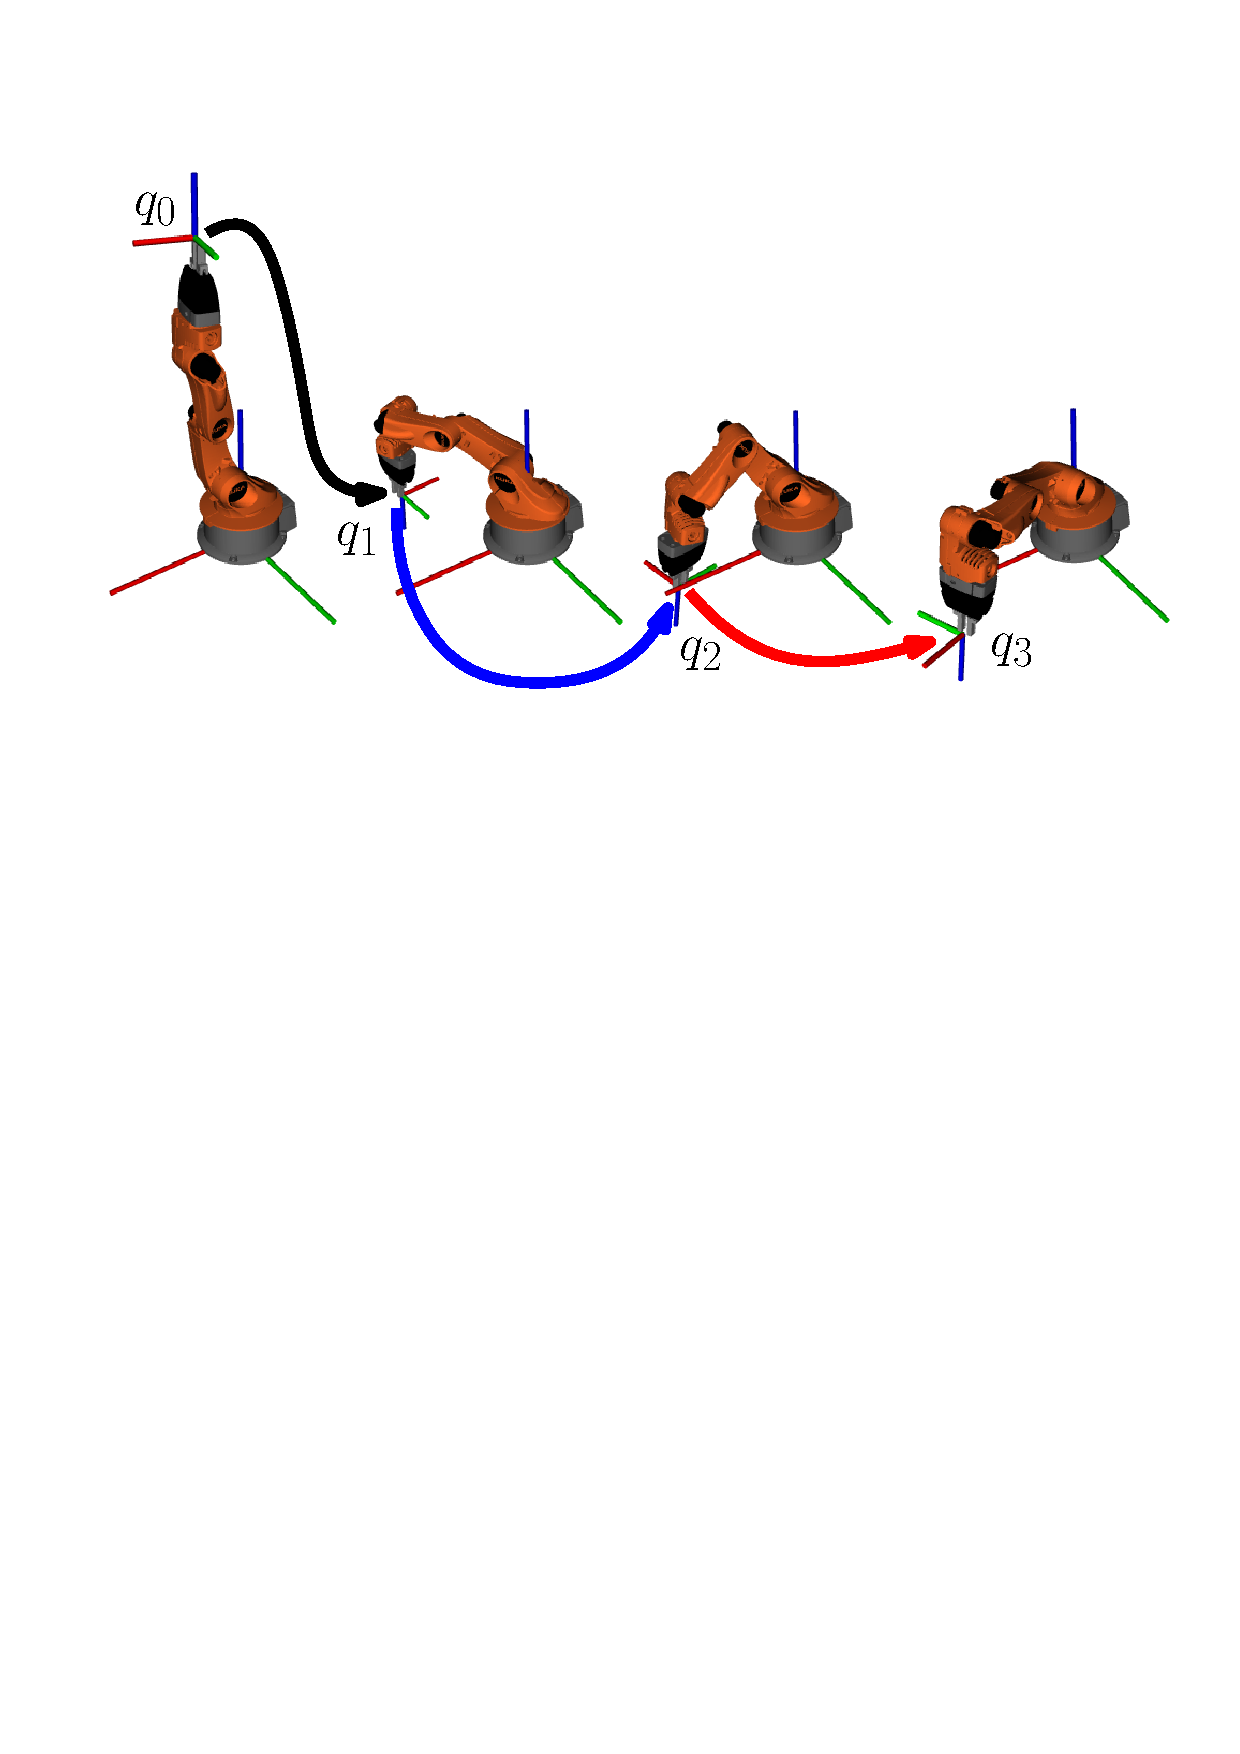
\includegraphics[width=1\textwidth]{modeling/poses.pdf}}
	\caption{Последовательность принятия положений заданных в~\ref{poses_q}}
	\vspace{0.5cm}
	\label{img:poses}
\end{figure}
\begin{gather}\label{poses_q}
	q_0 = 
	\begin{bmatrix}
	2.95 \\ 1.35 \\-2.59 \\1.58\\ 0
	\end{bmatrix}\!\!,\quad
	q_1 =
	\begin{bmatrix}
		 4.06 \\ 2.34\\ -2.2\\ 3.32\\ 1.01
	\end{bmatrix}\!\!,\quad
	q_2 = 
	\begin{bmatrix}
	3.07 \\1.75\\ -0.93 \\2.54\\ 1.73
	\end{bmatrix}\!\!,\quad
	q_3 = 
	\begin{bmatrix}
	2.57\\ 2.33\\ -2.35\\ 3.36\\ 2.97
	\end{bmatrix}\!\!.
\end{gather}

На рисунках~\ref{img:segments_traj} и~\ref{img:polyn_traj} показаны графики переходных процессов для переходов из точки в точку при планировании траектории сегментами и использовании полинома пятой степени соответственно.

\begin{figure}[h!]
	\centering{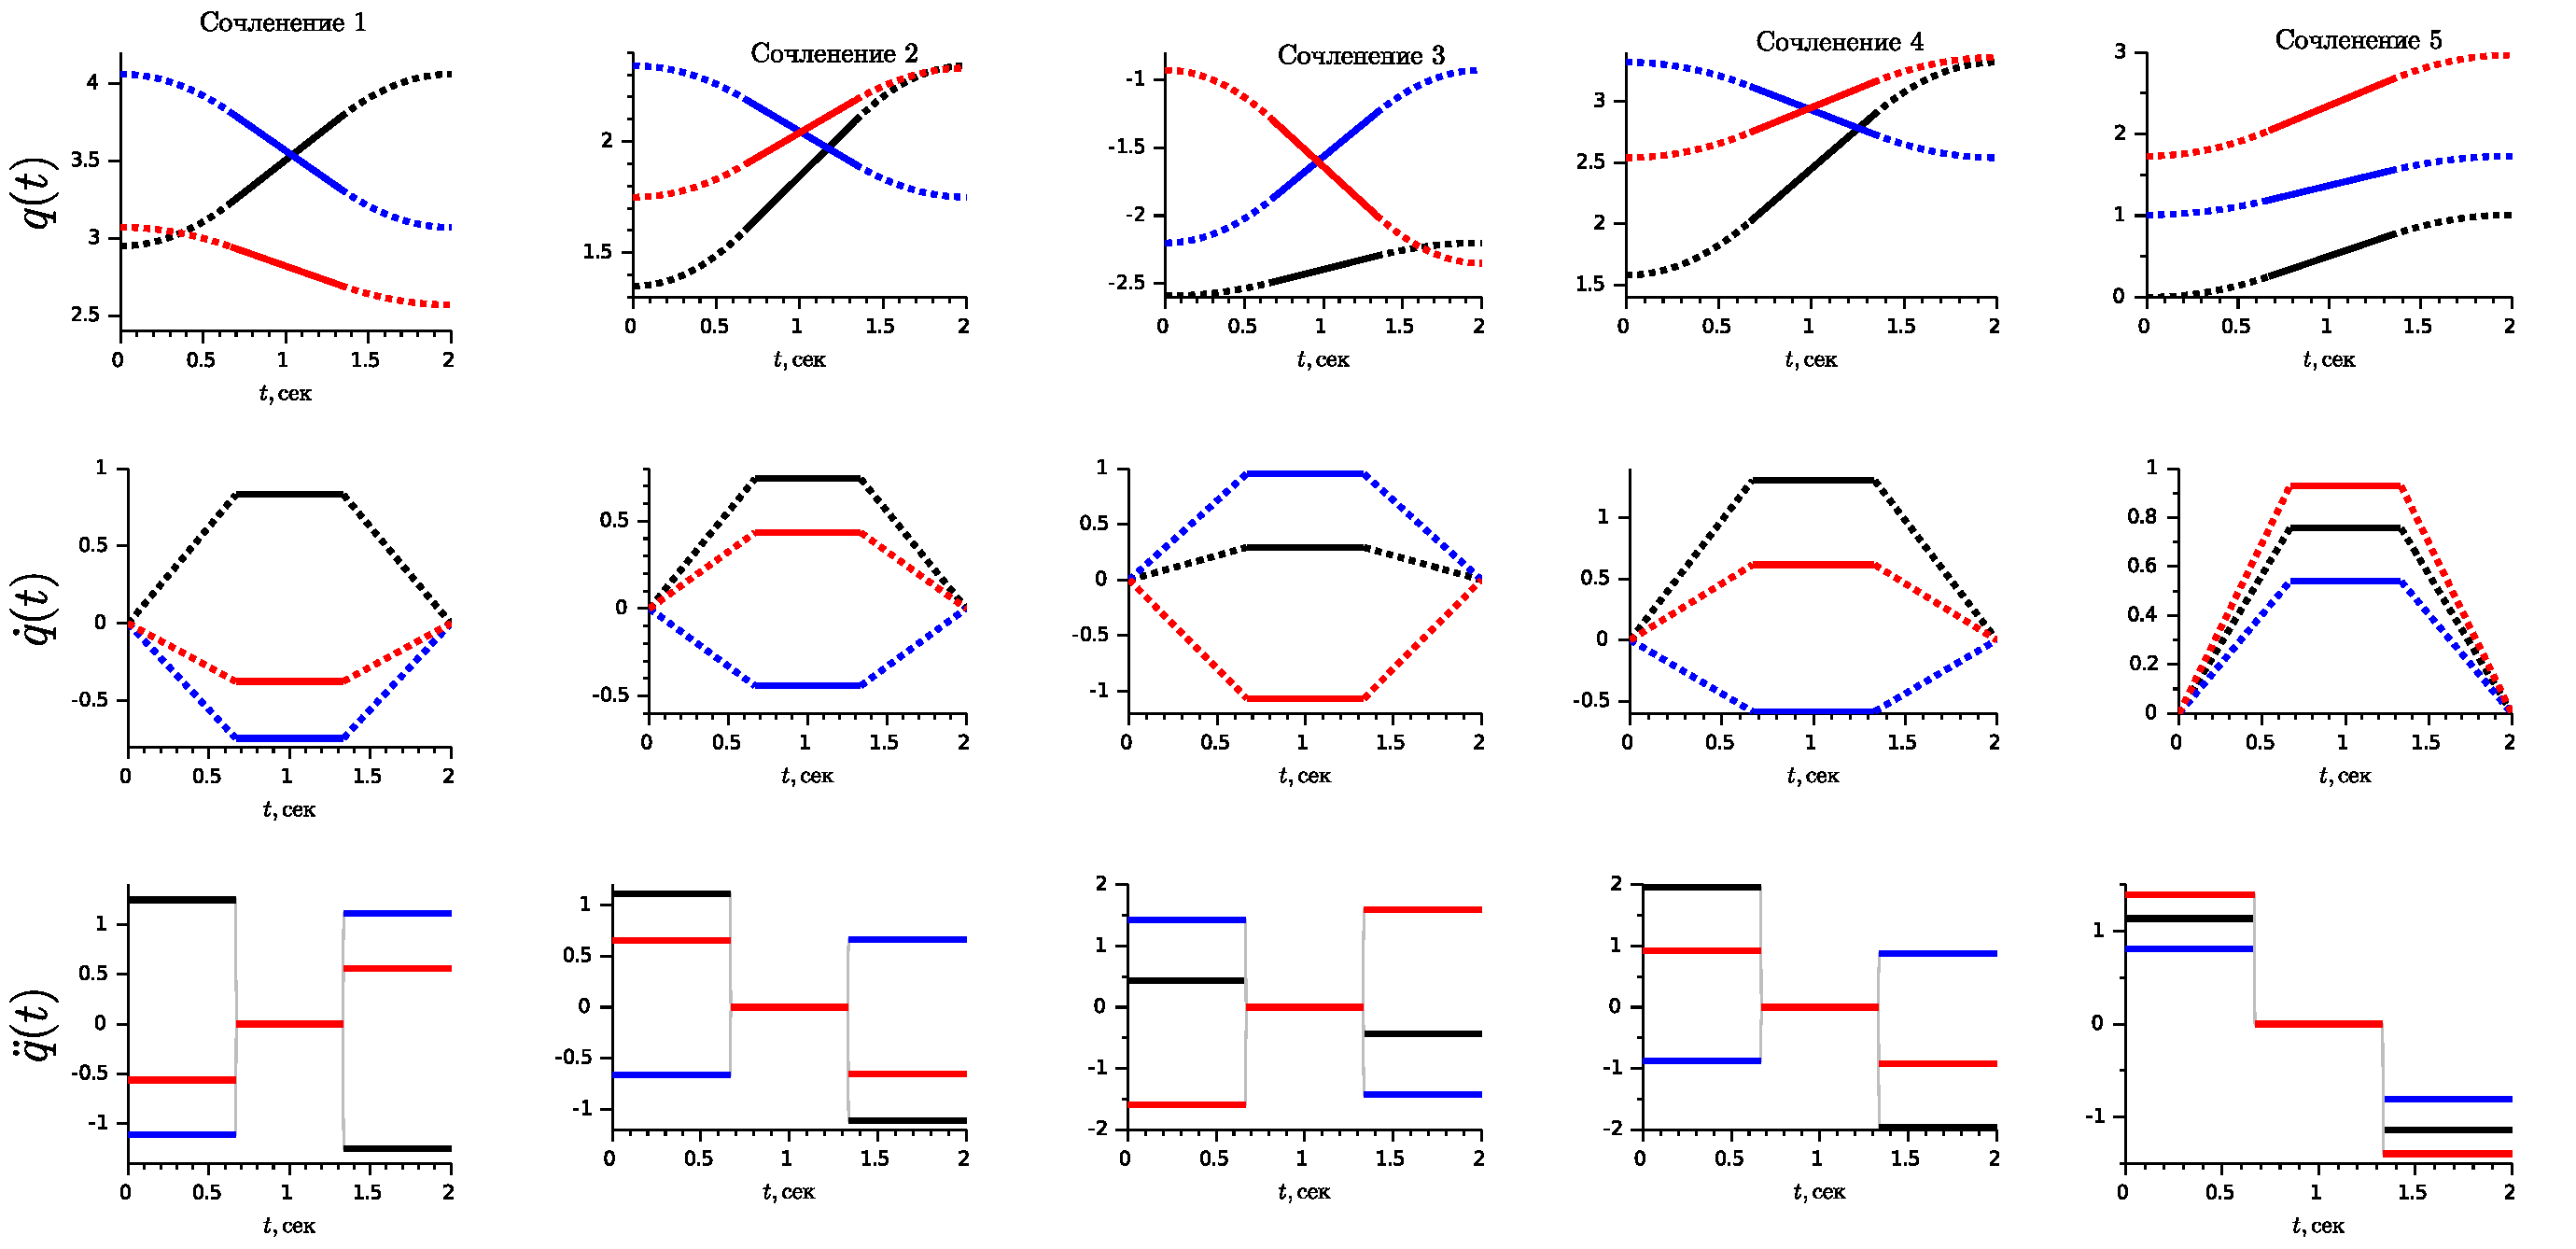
\includegraphics[width=1\textwidth]{modeling/seg_traj.pdf}
		\small черный: для перехода $ q_0 \to q_1 $, \textcolor{blue}{синий: для перехода $ q_1 \to q_2 $}, \textcolor{red}{красный: для перехода $ q_2 \to q_3 $}}
	\vspace{0.2cm}
	\caption{Траектория с трапецеидальным профилем скорости}
	\label{img:segments_traj}
\end{figure}

\begin{figure}[h!]
	\centering{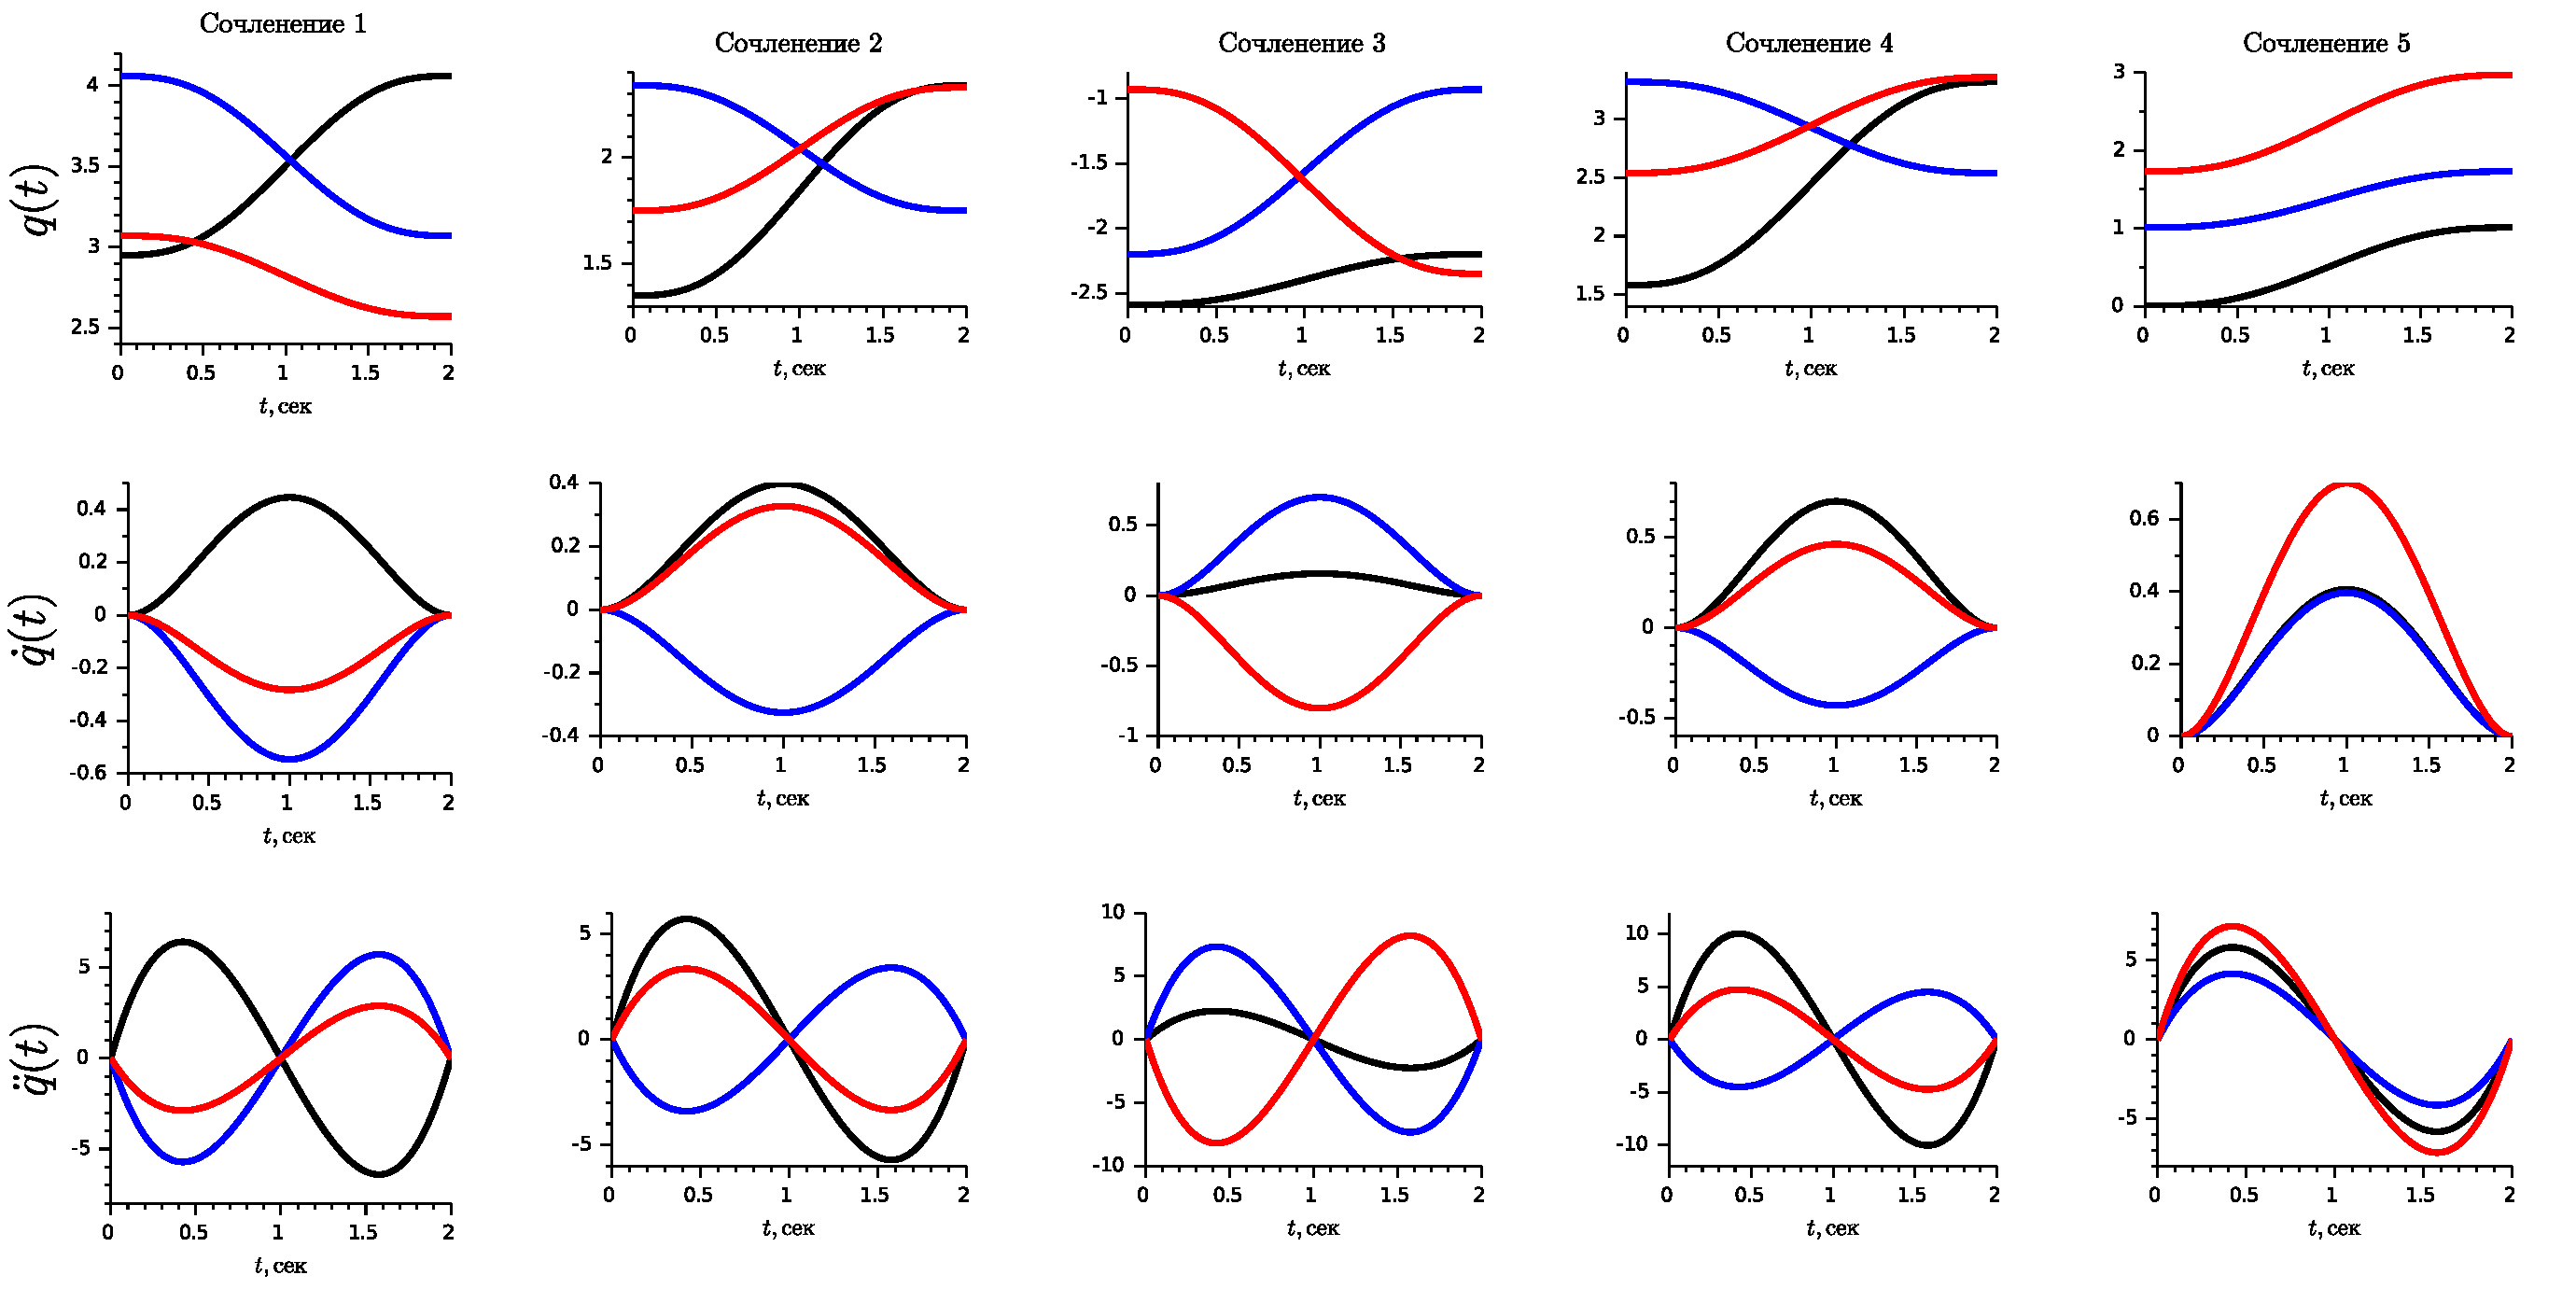
\includegraphics[width=1\textwidth]{modeling/poly_traj.pdf}
		\small черный: для перехода $ q_0 \to q_1 $, \textcolor{blue}{синий: для перехода $ q_1 \to q_2 $}, \textcolor{red}{красный: для перехода $ q_2 \to q_3 $}}
	\vspace{0.2cm}
	\caption{Траектория при полиномиальной интерполяции}
	\label{img:polyn_traj}
\end{figure}

\begin{figure}[h!]
	\centering{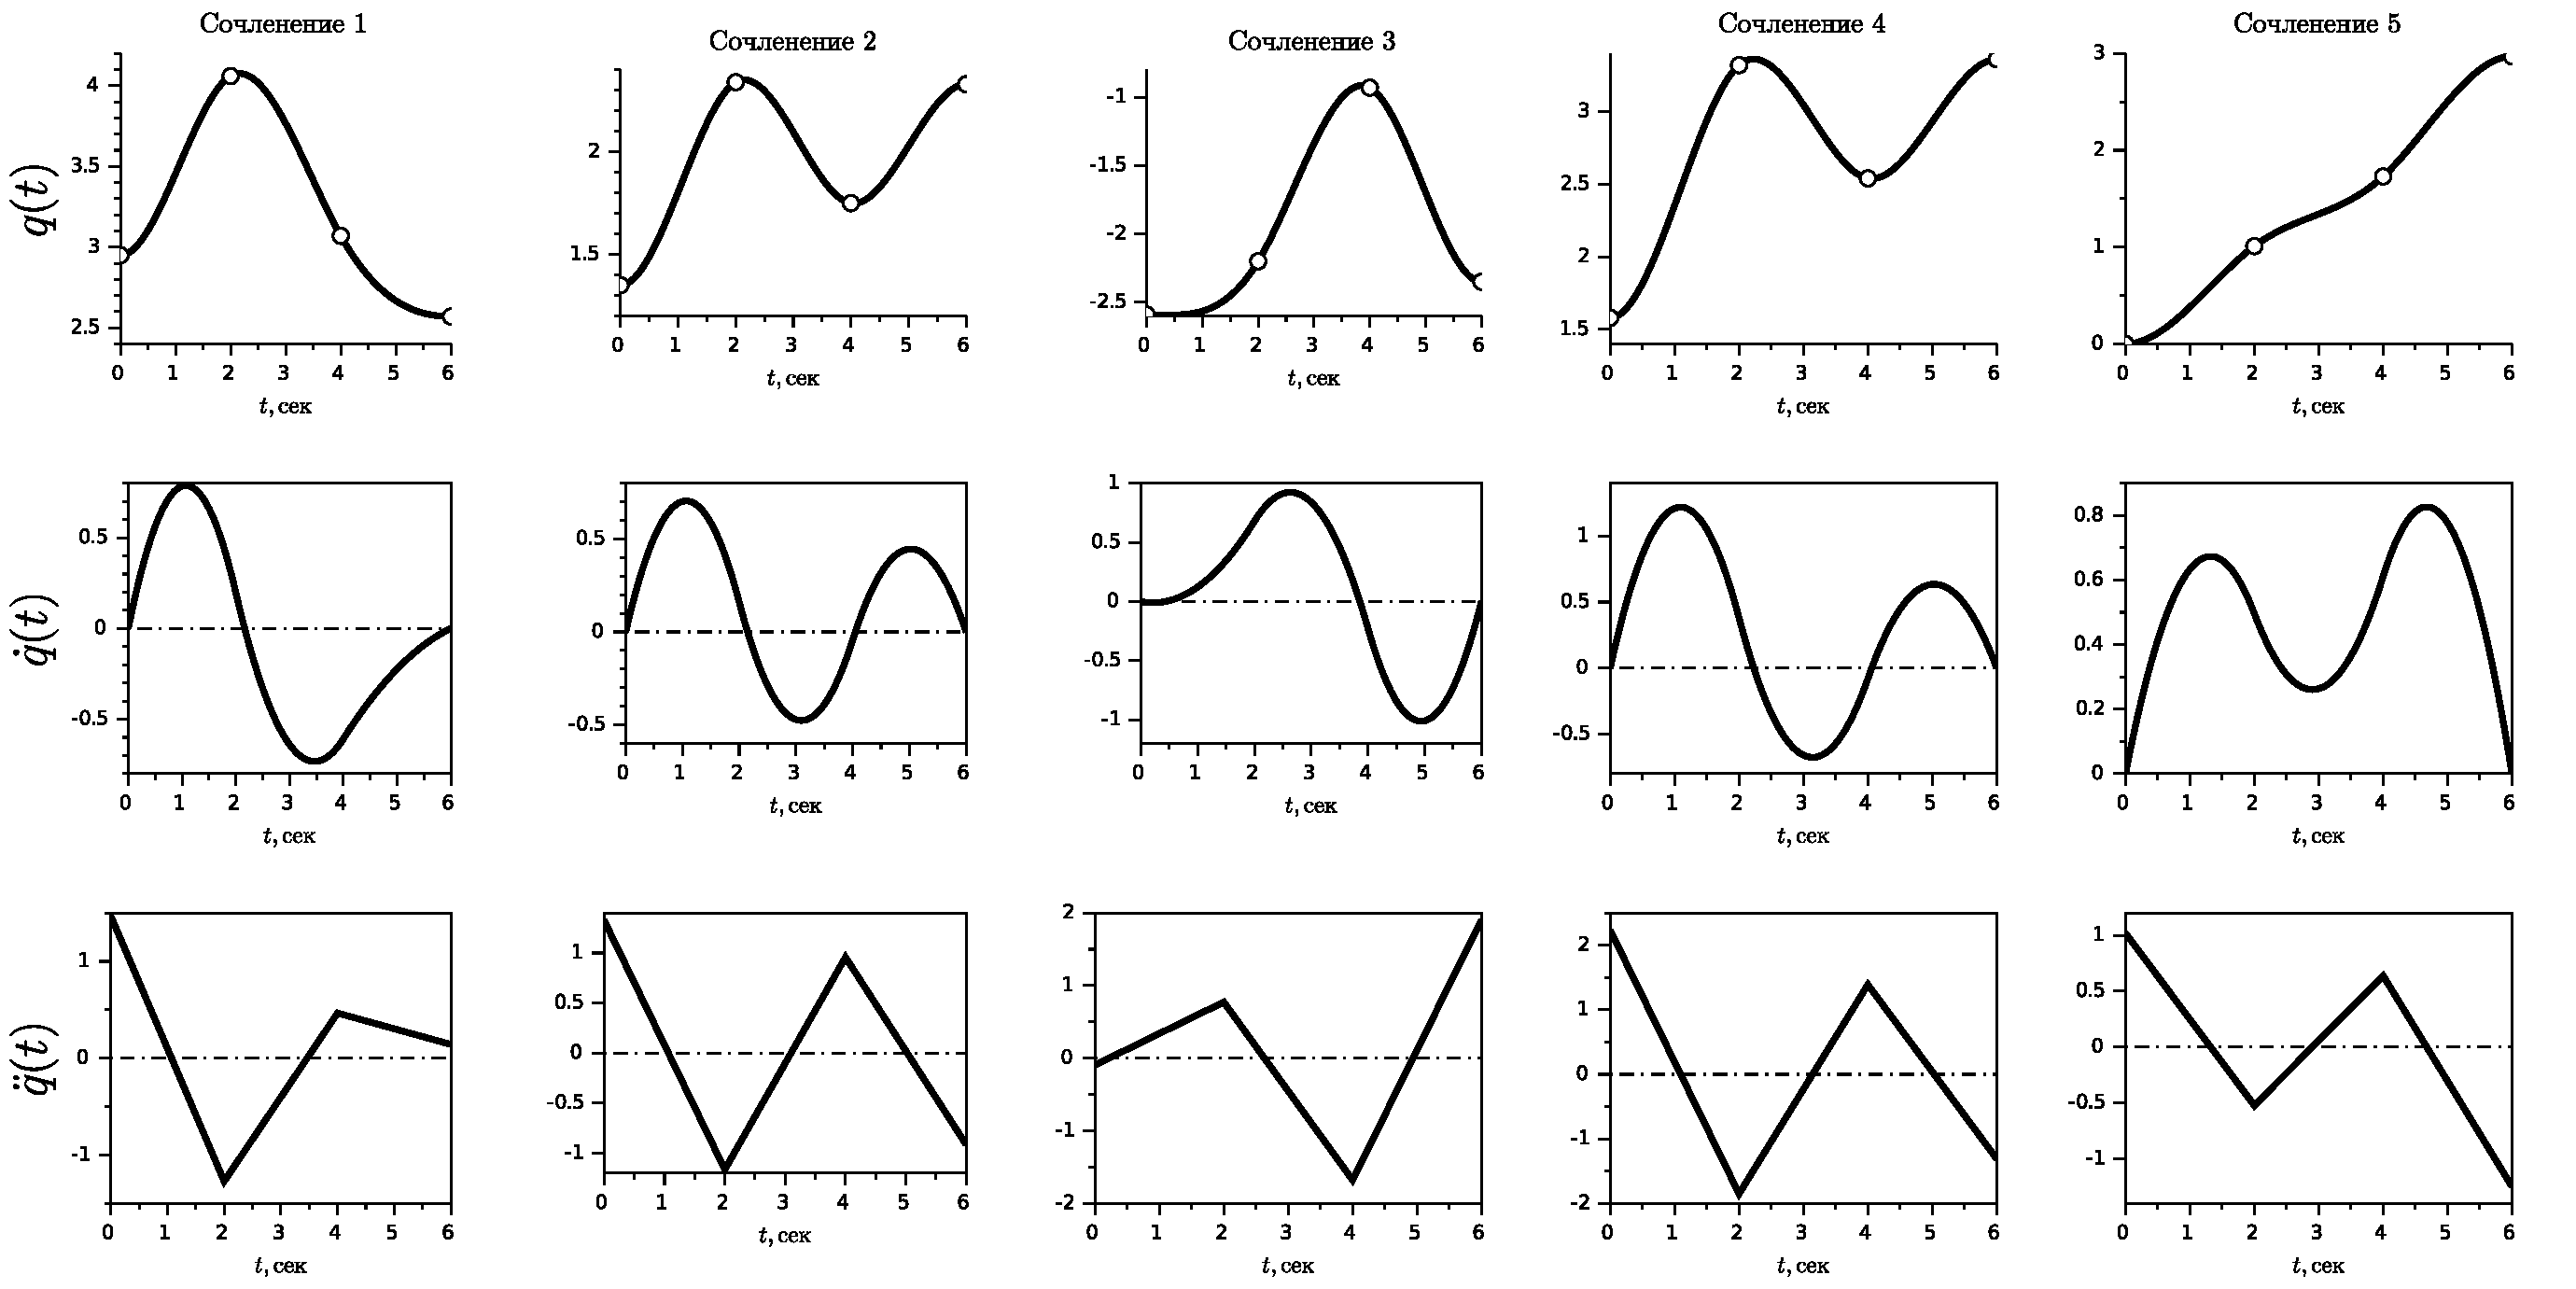
\includegraphics[width=1\textwidth]{modeling/spline_traj.pdf}
		\small узлы на верхних графиках представляют из себя точки $ q_0(0), q_1(2), q_2(4), q_3(6) $}
	\vspace{0.2cm}
	\caption{Непрерывная траектория через набор точек}
	\label{img:spline_traj}
\end{figure}

Траектория (дуга) в операционном пространстве и соответствующие ей траектории каждого из сочленений в конфигурационном пространстве представлены на рисунке~\ref{img:cartesian}.

\begin{figure}[h!]
	\centering{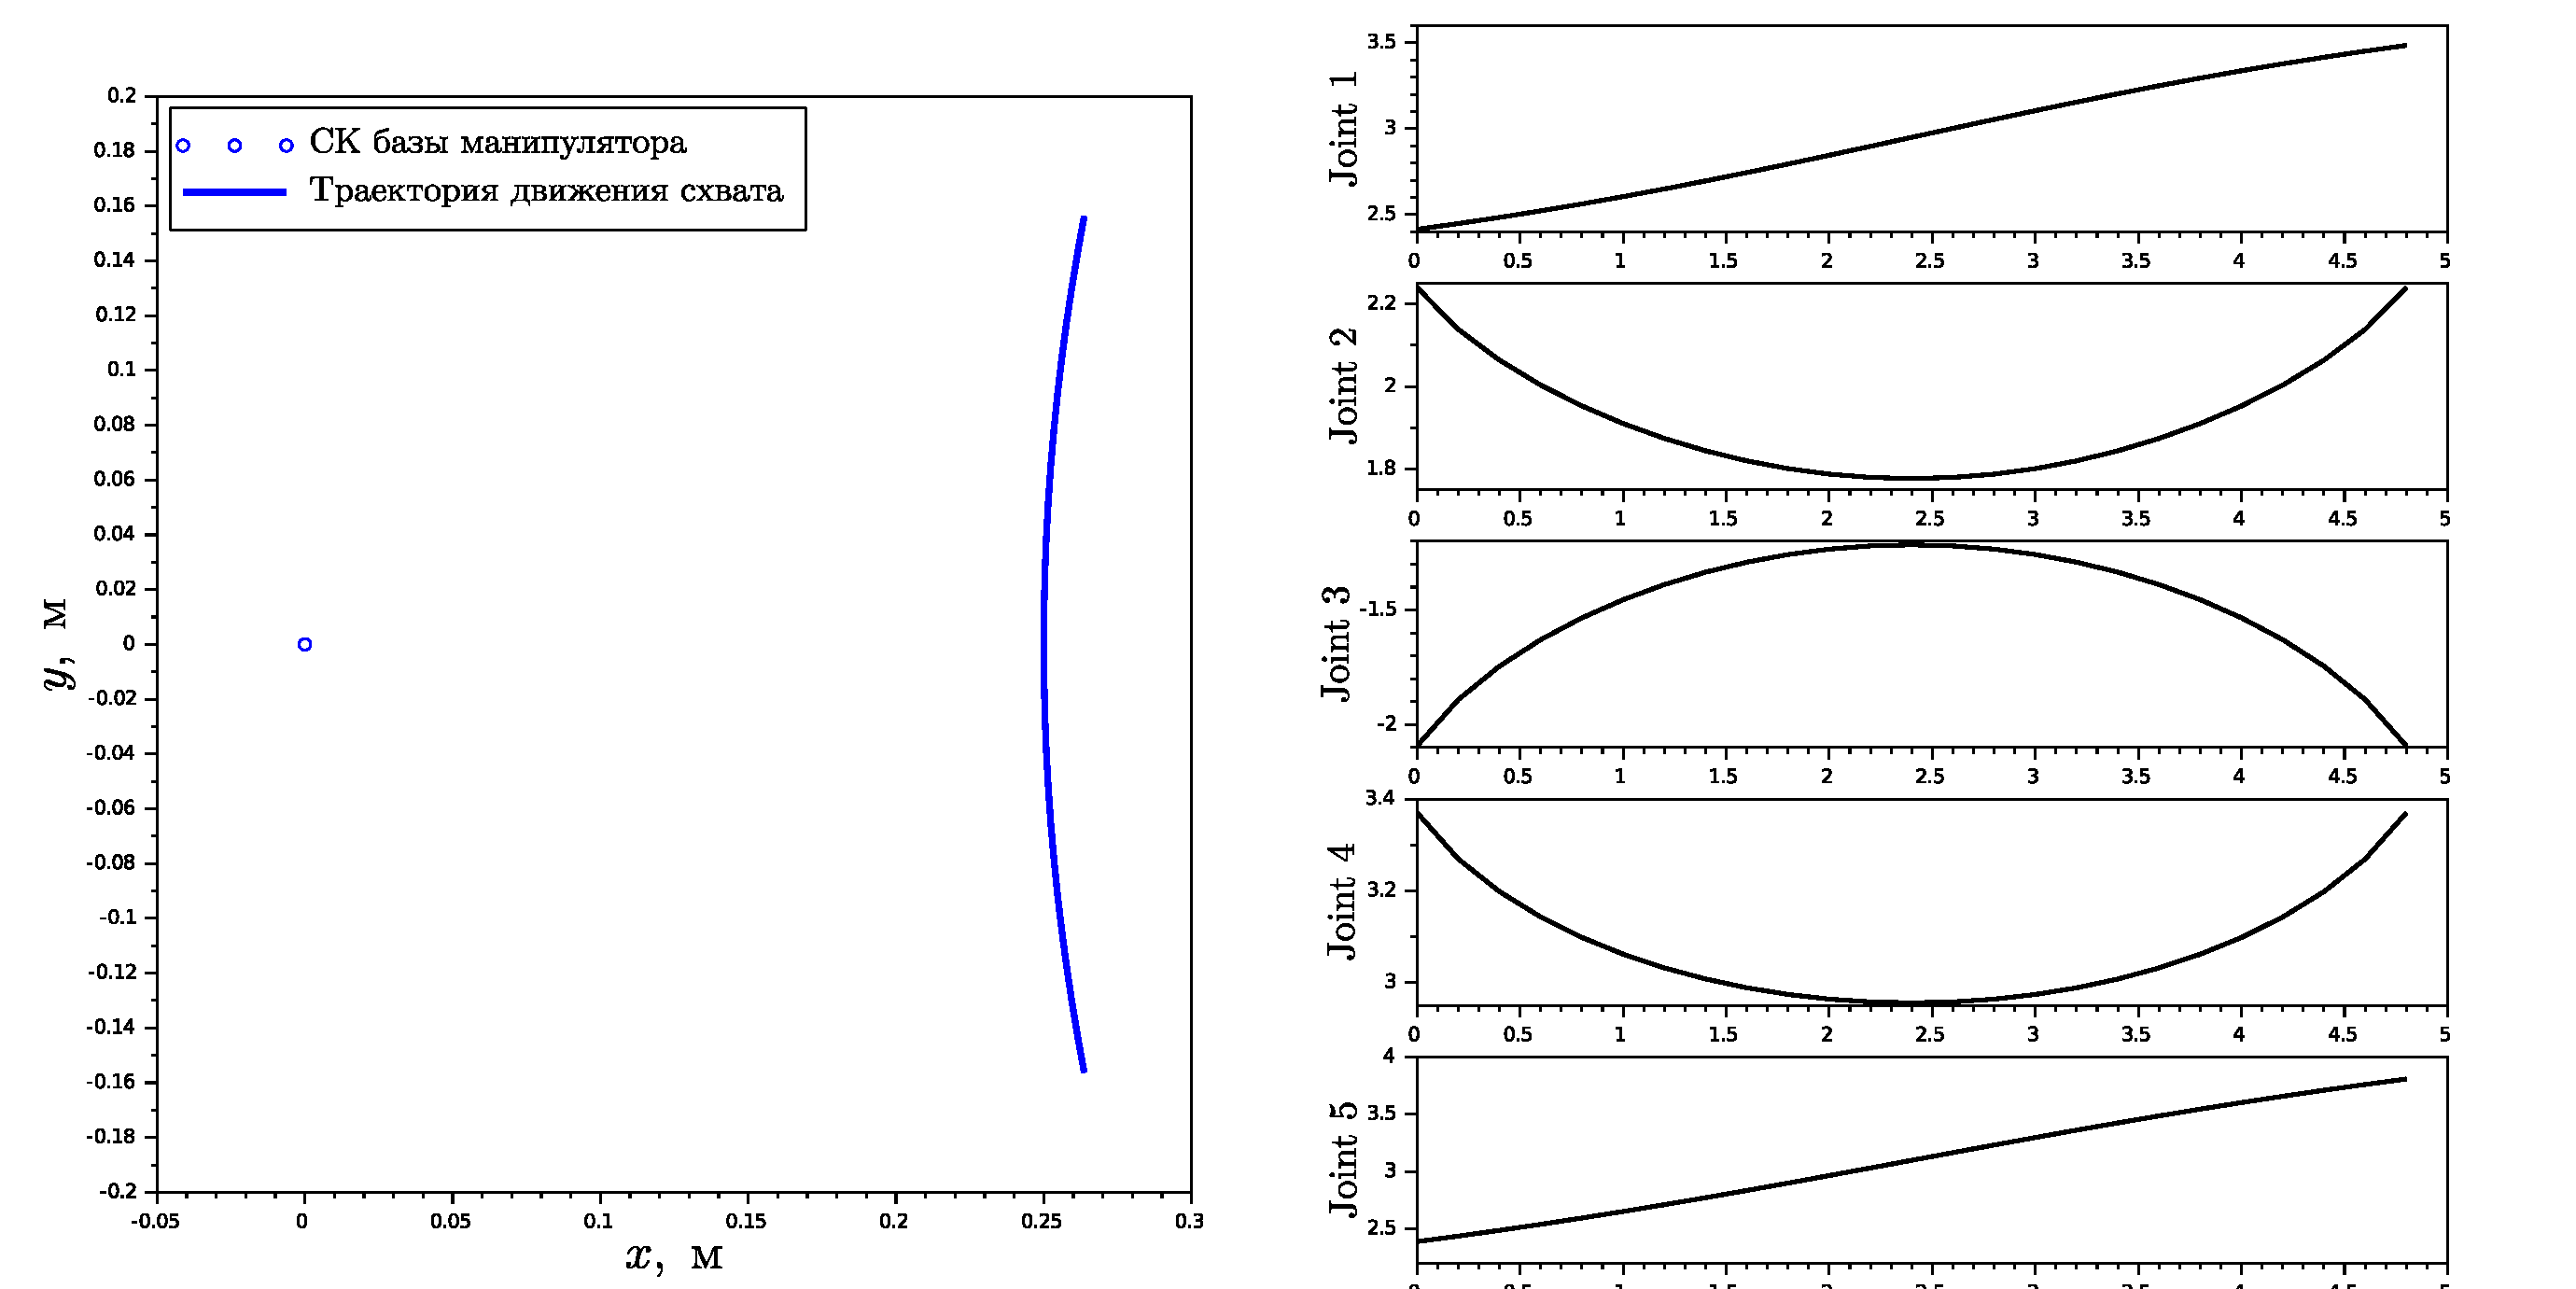
\includegraphics[width=1\textwidth]{modeling/cartesian.pdf}}
	\vspace{0.2cm}
	\caption{Траектория движения схвата манипулятора и соответствующие ей траектории сочленений в конфигурационном пространстве}
	\label{img:cartesian}
\end{figure}

\begin{figure}[h!]
	\centering{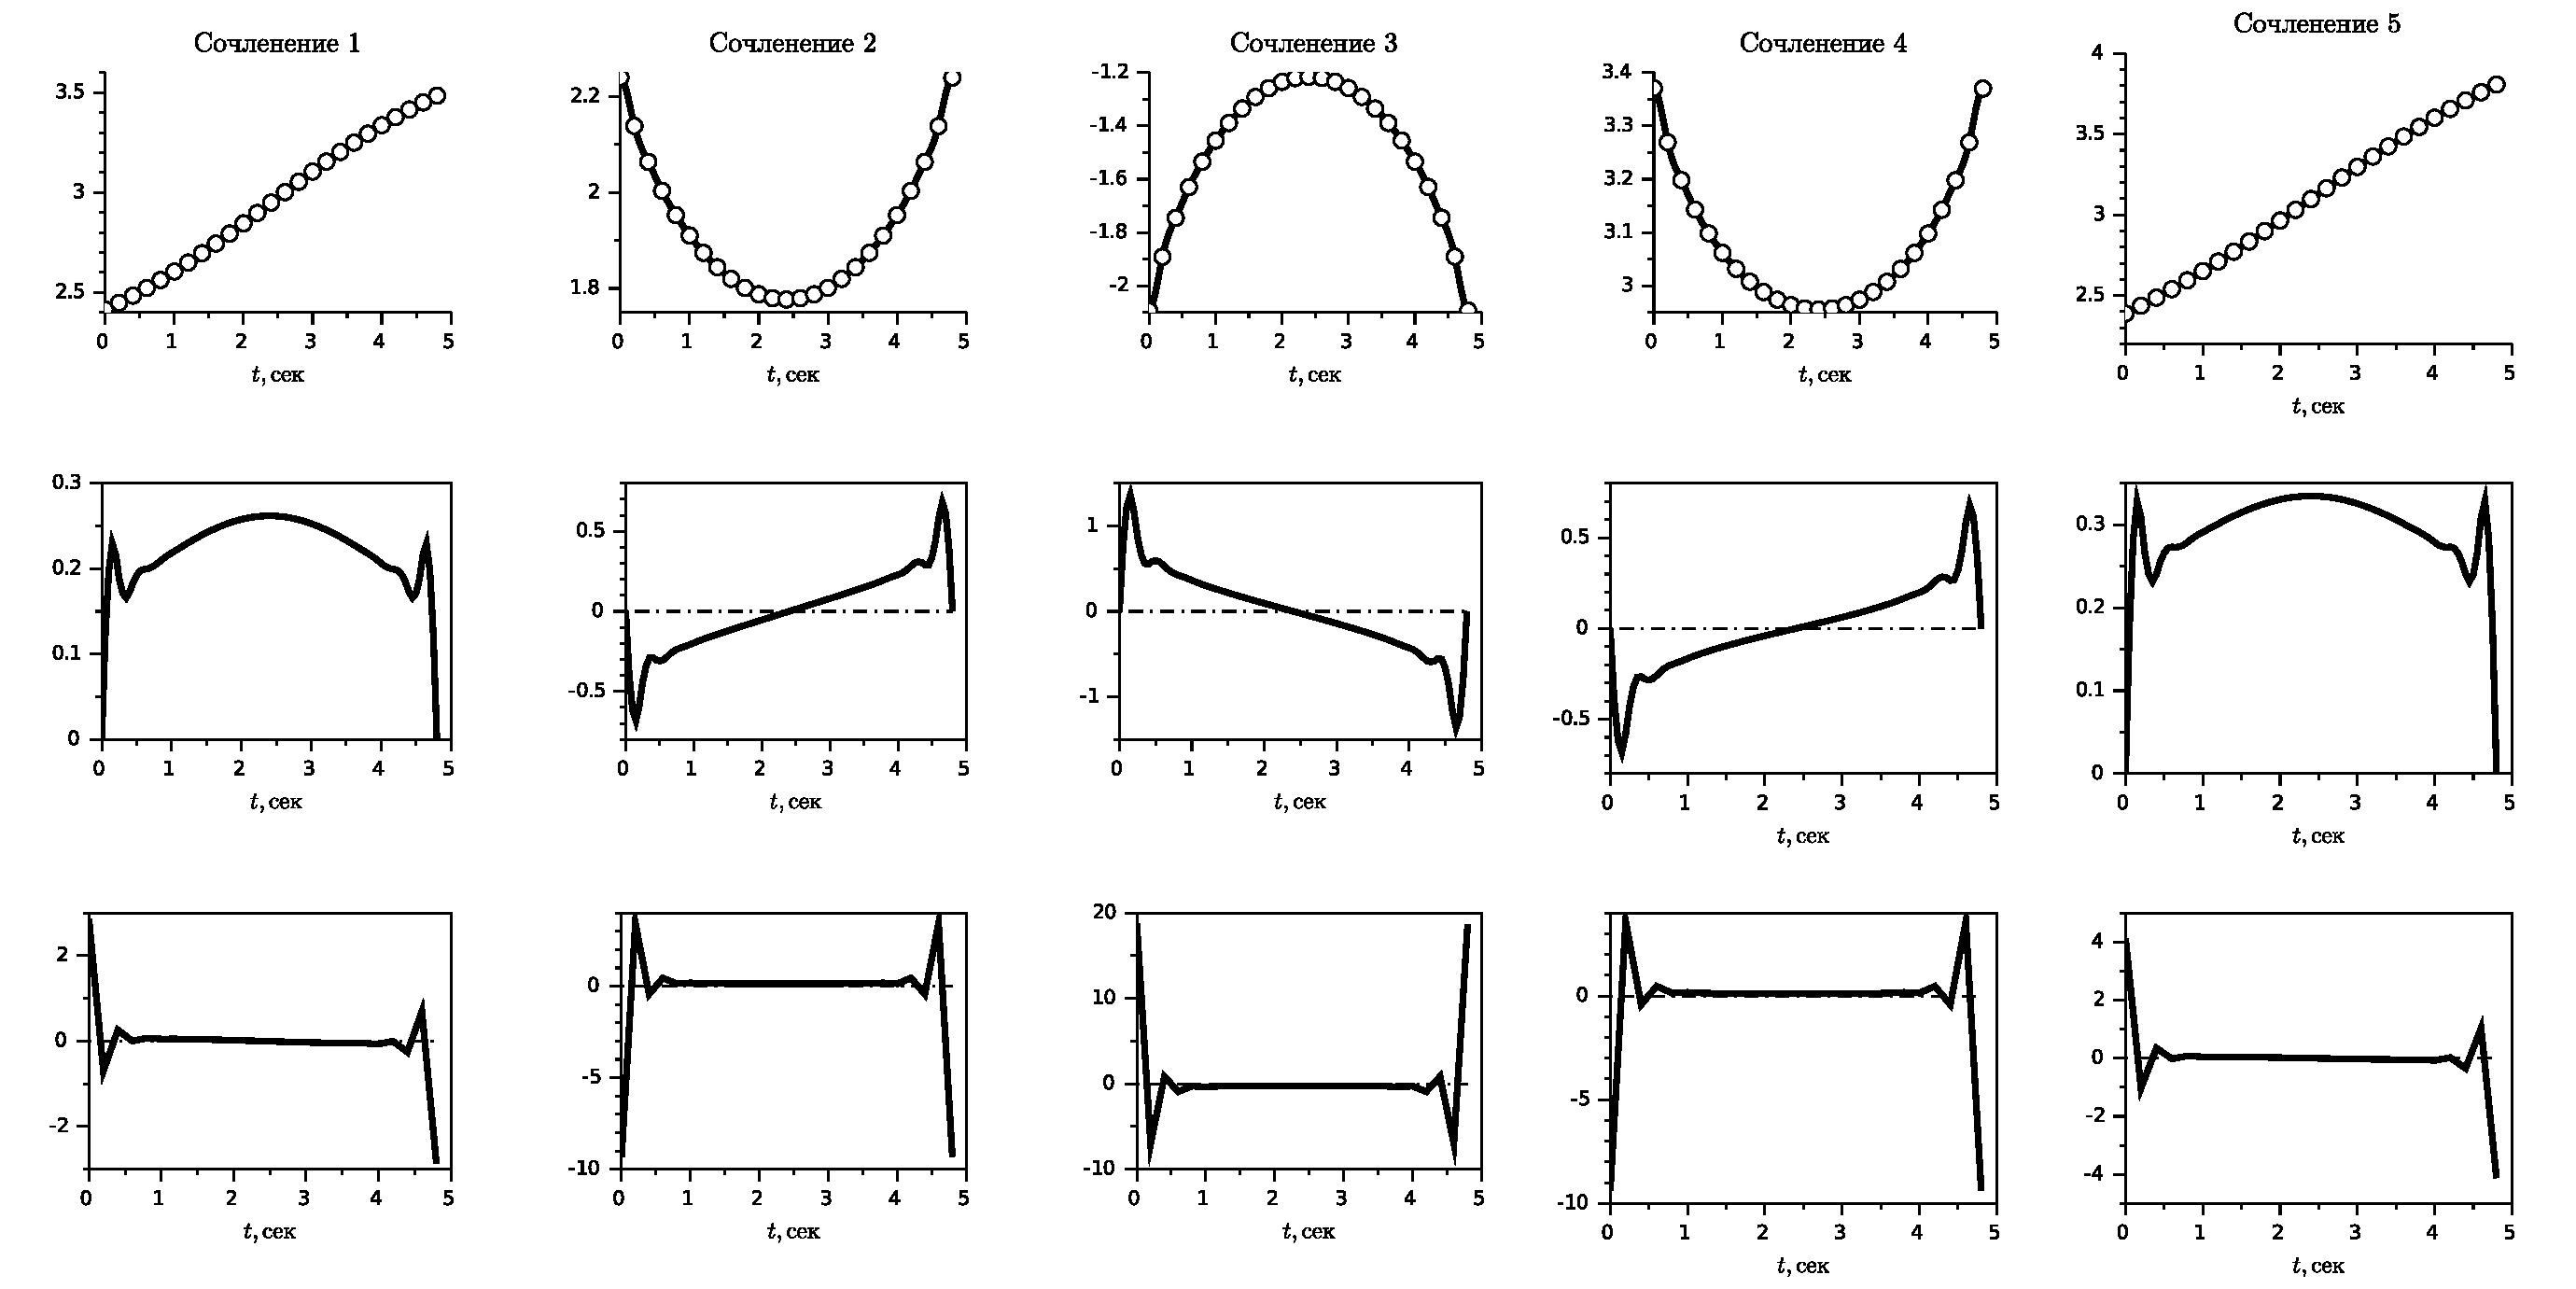
\includegraphics[width=1\textwidth]{modeling/js_cartesian.pdf}}
	\vspace{0.2cm}
	\caption{Интерполяция траекторий кубическими сплайнами}
	\label{img:js_cartesian}
\end{figure}

\clearpage

\subsection{Моделирование системы управления манипулятором}

\begin{figure}[h!]
	\centering{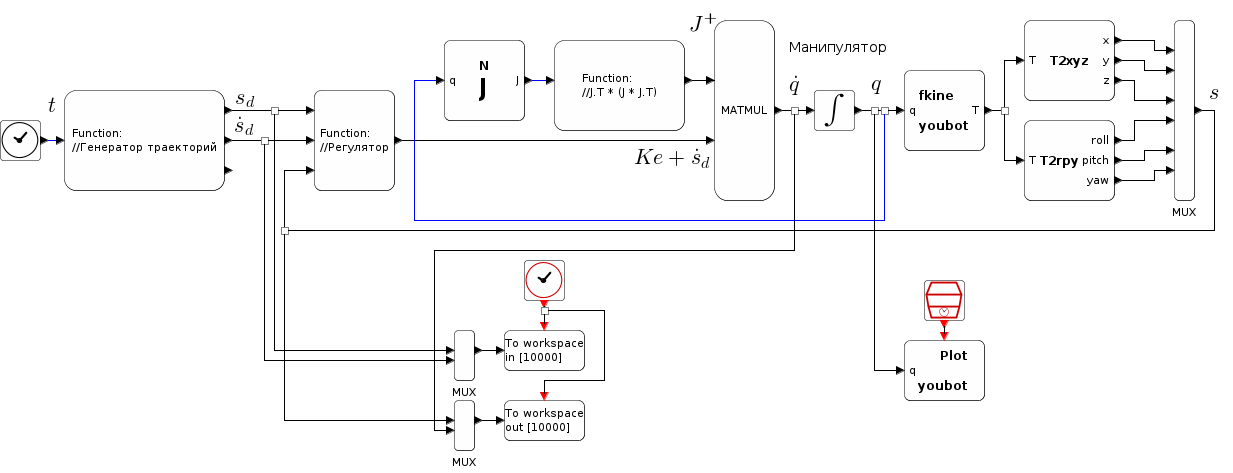
\includegraphics[width=0.95\textwidth]{modeling/control_system.png}}
	\caption{Модель системы управления манипуляторов в Scilab}
	\label{img:control_system}
\end{figure}

\begin{figure}[h!]
	\begin{minipage}[h]{0.5\linewidth}
		\centering{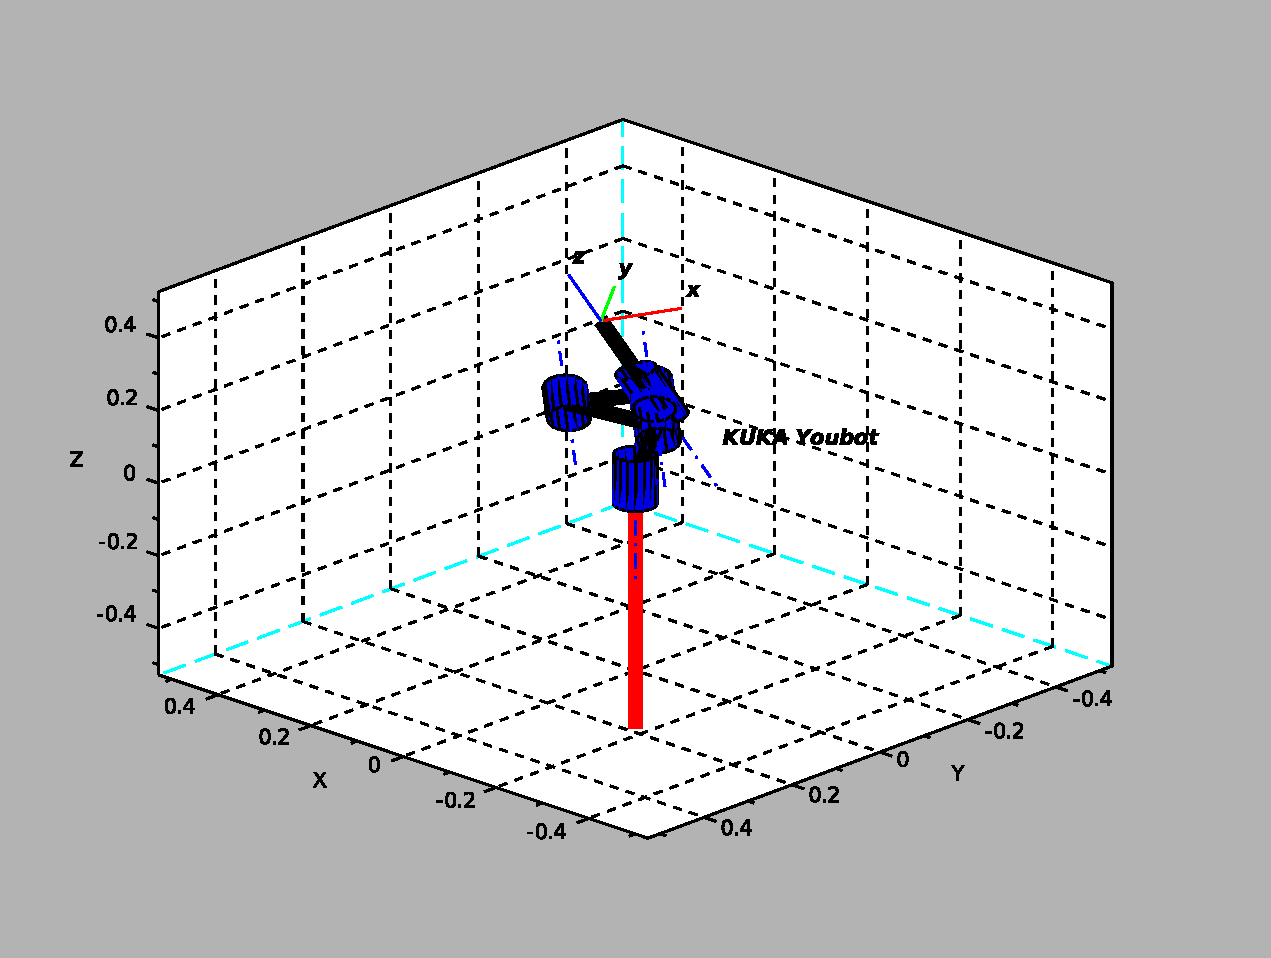
\includegraphics[width=1\linewidth]{modeling/model1.pdf} \\ а)}
	\end{minipage}
	\hfill
	\begin{minipage}[h]{0.5\linewidth}
		\centering{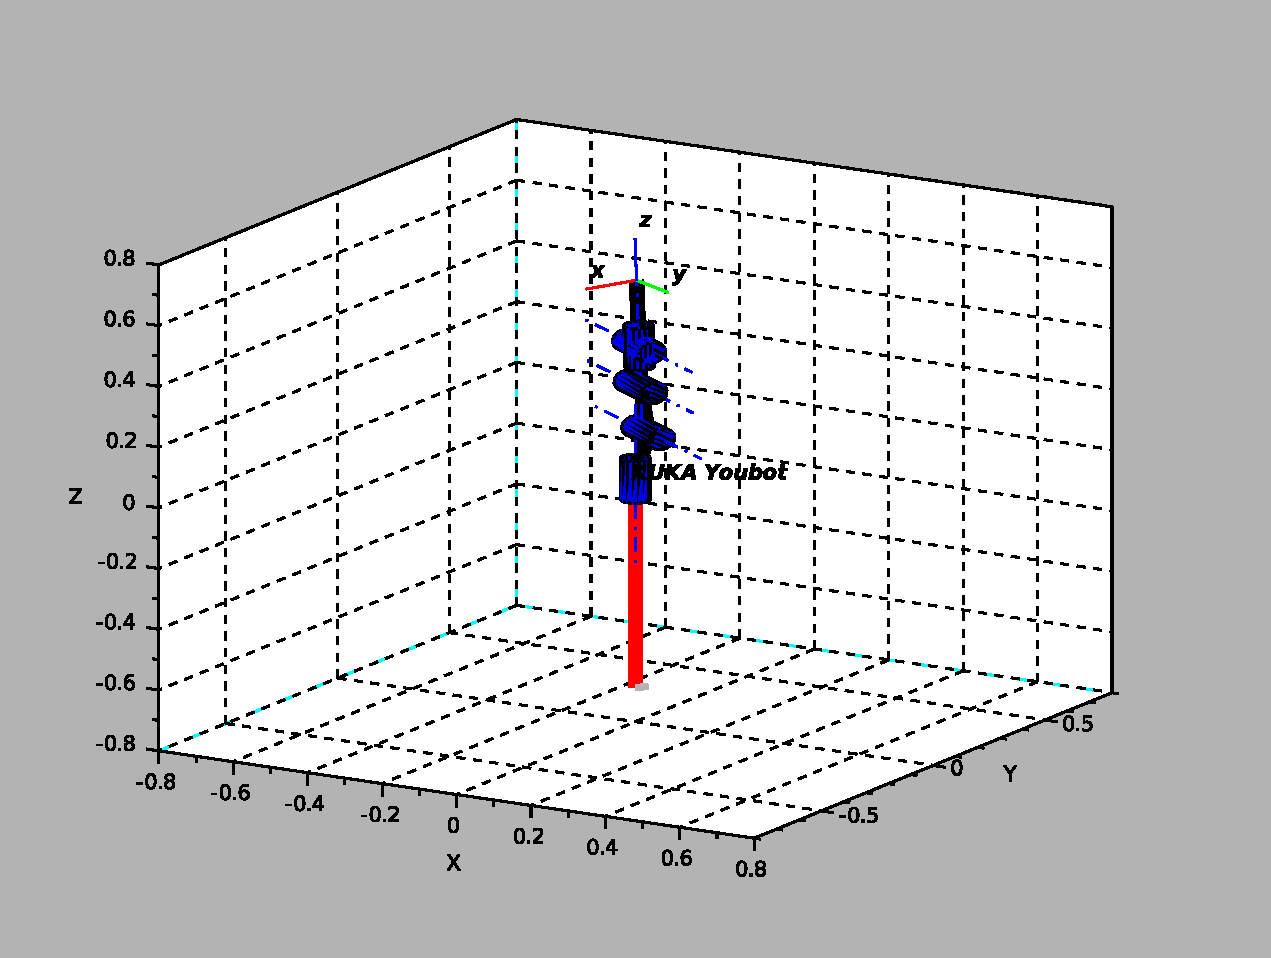
\includegraphics[width=1\linewidth]{modeling/model2.pdf} \\ б)}
	\end{minipage}
	\caption{a) Манипулятор KUKA YouBot в "домашней" конфигурации; б) В свече}
	\label{img:model}
\end{figure}

\subsection{Результаты работы системы технического зрения}

Путь получения координат и ориентации объекта покажем на нижеследующей последовательности рисунков. На рисунке~\ref{img:raw_cloud} изображено облако точек, полученное с камеры Intel RealSense SR300. После фильтрации этого облака, получается облако с пониженным качеством и показывается на рисунке~\ref{img:downsampled_cloud}. Далее, на рисунке~\ref{img:downsampled_cloud}б, изображена плоскость~--- результат работы алгоритма сегментации. Следующий рисунок~\ref{img:hull}а содержит результат нахождения выпуклой оболочки вокруг плоскости. И, облако точек целевого объекта, показоно на рисунке~\ref{img:hull}б. Рисунок~\ref{img:frame} включает плоскость, объект и СК прикрепленную к объекту.

\begin{figure}[h!]
	\begin{minipage}[h]{0.5\linewidth}
		\centering{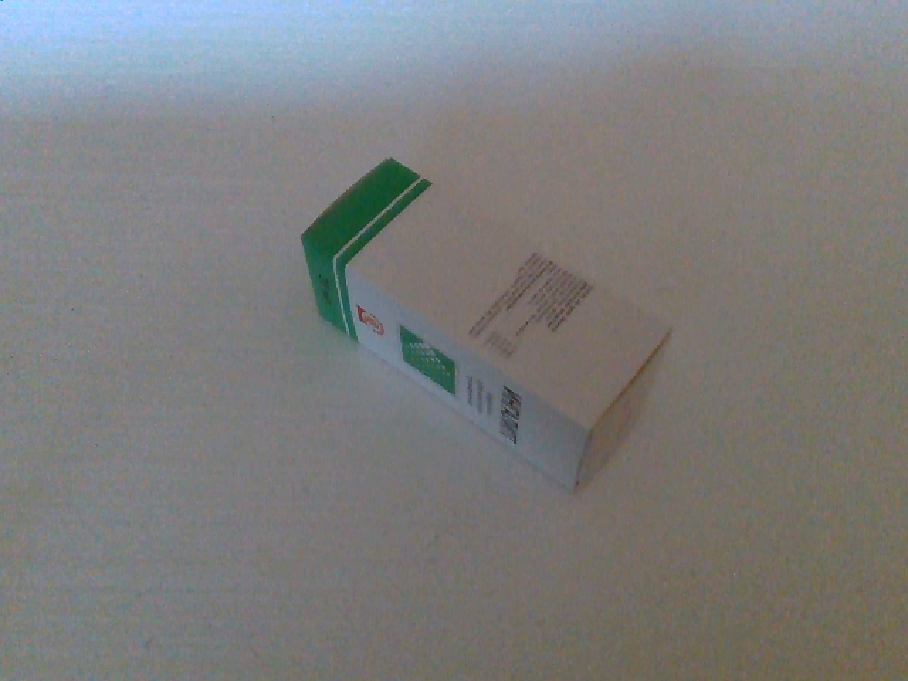
\includegraphics[width=0.7\linewidth]{modeling/cv_image.png} \\ а)}
	\end{minipage}
	\hfill
	\begin{minipage}[h]{0.5\linewidth}
		\centering{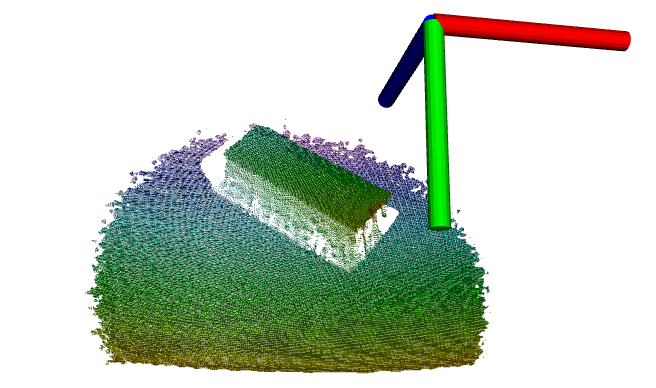
\includegraphics[width=1\linewidth]{modeling/cv_raw_cloud.png} \\ б)}
	\end{minipage}
	\caption{a) Цветное изображение целевого объекта; б) Необработанное облако точек}
	\label{img:raw_cloud}
\end{figure}

\begin{figure}[h!]
	\begin{minipage}[h]{0.5\linewidth}
		\centering{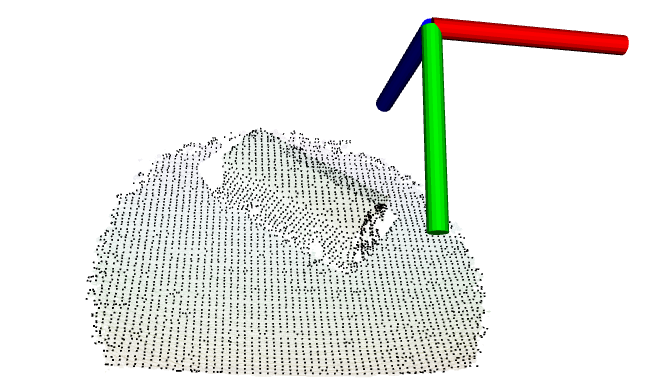
\includegraphics[width=1\linewidth]{modeling/_cv_raw_ds.png} \\ а)}
	\end{minipage}
	\hfill
	\begin{minipage}[h]{0.5\linewidth}
		\centering{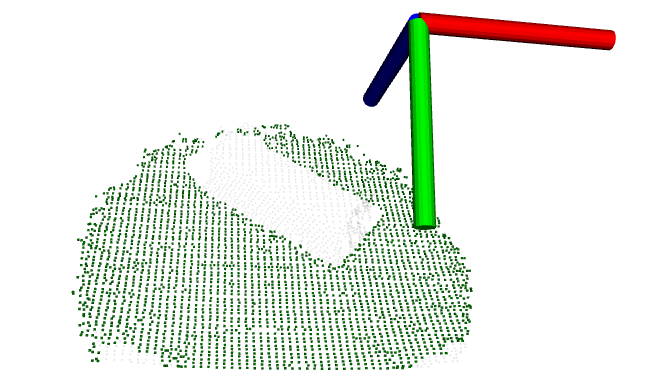
\includegraphics[width=1\linewidth]{modeling/_cv_ds2plane.png} \\ б)}
	\end{minipage}
	\caption{а) Облако точек пропущенное через фильтр VoxelGrid; б) Часть облака точек принадлежащая плоскости в кадре самой большой площади}
	\label{img:downsampled_cloud}
\end{figure}

\begin{figure}[h!]
	\begin{minipage}[h]{0.5\linewidth}
		\centering{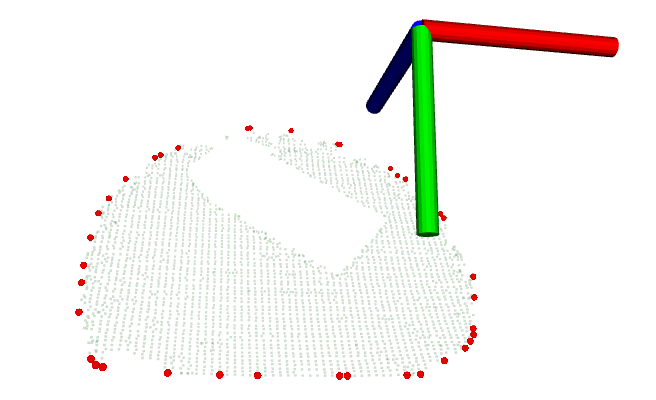
\includegraphics[width=1\linewidth]{modeling/_cv_plane2hull.png} \\ а)}
	\end{minipage}
	\hfill
	\begin{minipage}[h]{0.5\linewidth}
		\centering{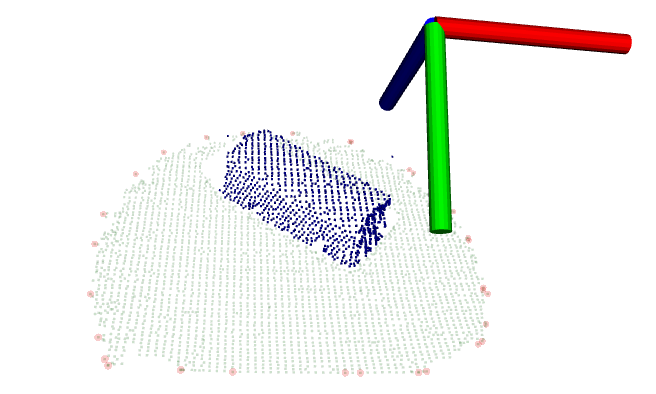
\includegraphics[width=1\linewidth]{modeling/_cv_2object.png} \\ б)}
	\end{minipage}
	\caption{а) Точки принадлежащие выпуклой оболочке, вокруг плоскости; б) Кластер облака точек включающих только целевой объект}
	\label{img:hull}
\end{figure}

\begin{figure}[h!]
	\centering{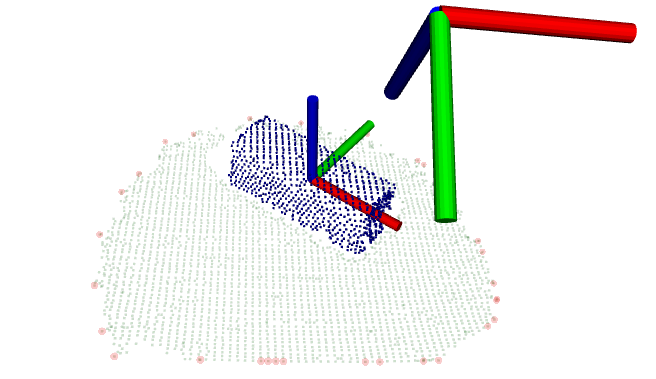
\includegraphics[width=1\textwidth]{modeling/cv_frame.png}}
	\vspace{0.2cm}
	\caption{Прикрепленная к объекту СК}
	\label{img:frame}
\end{figure}

\clearpage
\newpage
\section*{Заключение}
\addcontentsline{toc}{section}{Заключение}
Текст заключения
\newpage



\renewcommand\refname{Список использованных источников}
\providecommand*{\url}[1]{#1} %нужно для описания некоторых источников

\bibliography{used_books}
\ESKDappendix{обязательное}{Название приложения}\label{append_app_example}
Текст приложения


\end{document}
